%%%%%%%%%%%%%%%%%%%%%%%%%%%%%%%%%%%%%%%%%
% Beamer Presentation
% LaTeX Template
% Version 1.0 (10/11/12)
%
% This template has been downloaded from:
% http://www.LaTeXTemplates.com
%
% License:
% CC BY-NC-SA 3.0 (http://creativecommons.org/licenses/by-nc-sa/3.0/)
%
%%%%%%%%%%%%%%%%%%%%%%%%%%%%%%%%%%%%%%%%%

%----------------------------------------------------------------------------------------
%	PACKAGES AND THEMES
%----------------------------------------------------------------------------------------

\documentclass[aspectratio=169]{beamer}
%%\documentclass{beamer}
\mode<presentation> {

% The Beamer class comes with a number of default slide themes
% which change the colors and layouts of slides. Below this is a list
% of all the themes, uncomment each in turn to see what they look like.

%\usetheme{default}
%\usetheme{AnnArbor}
%\usetheme{Antibes}
%\usetheme{Bergen}
%\usetheme{Berkeley}
%\usetheme{Berlin}
%\usetheme{Boadilla}
%\usetheme{CambridgeUS}
%\usetheme{Copenhagen}
%\usetheme{Darmstadt}
%\usetheme{Dresden}
%\usetheme{Frankfurt}
%\usetheme{Goettingen}
%\usetheme{Hannover}
%\usetheme{Ilmenau}
%\usetheme{JuanLesPins}
%\usetheme{Luebeck}
\usetheme{Madrid}
%\usetheme{Malmoe}
%\usetheme{Marburg}
%\usetheme{Montpellier}
%\usetheme{PaloAlto}
%\usetheme{Pittsburgh}
%\usetheme{Rochester}
%\usetheme{Singapore}
%\usetheme{Szeged}
%\usetheme{Warsaw}

% As well as themes, the Beamer class has a number of color themes
% for any slide theme. Uncomment each of these in turn to see how it
% changes the colors of your current slide theme.

%\usecolortheme{albatross}
%\usecolortheme{beaver}
%\usecolortheme{beetle}
%\usecolortheme{crane}
%\usecolortheme{dolphin}
%\usecolortheme{dove}
%\usecolortheme{fly}
%\usecolortheme{lily}
%\usecolortheme{orchid}
%\usecolortheme{rose}
%\usecolortheme{seagull}
%\usecolortheme{seahorse}
%\usecolortheme{whale}
%\usecolortheme{wolverine}

%\setbeamertemplate{footline} % To remove the footer line in all slides uncomment this line
%\setbeamertemplate{footline}[page number] % To replace the footer line in all slides with a simple slide count uncomment this line

%\setbeamertemplate{navigation symbols}{} % To remove the navigation symbols from the bottom of all slides uncomment this line
}
%%\documentclass[mathserif,hyperref={pdfpagemode=FullScreen}]{beamer}
%%% \documentclass[handout]{beamer}
%%% \usetheme{Dresden}
%%\usetheme{340}
%%\beamertemplatetransparentcovereddynamic
%%\usepackage[latin1]{inputenc}
%%\usepackage{pgf}


\usepackage{amsmath,amsfonts,amssymb}
\usepackage{xspace}
\usepackage{algorithm}
\usepackage{algorithmic}
\usepackage{xcolor}
\usepackage{graphicx} % Allows including images
\usepackage{booktabs} % Allows the use of \toprule, \midrule and \bottomrule in tables
%%\usepackage{xspace}

\usepackage{braket}
\usepackage{multirow}
\usepackage{todonotes}


%%\usepackage{enumitem}


\newcommand{\heteroprio}{{HeteroPrio}\xspace}
\newcommand{\heteroprioD}{{HeteroPrioDep}\xspace}


\usepackage{appendixnumberbeamer}

%%\usepackage{tcolorbox}
\usepackage{tikz}
\usetikzlibrary{matrix, decorations, patterns, positioning, shapes, calc, intersections, arrows, fit}


\usetikzlibrary{patterns}
\usetikzlibrary{fit,calc,positioning,decorations.pathreplacing,matrix}

\graphicspath{{./diagrams/}{./plots/}}

%%\tikzset{xtick/.style={inner xsep=0pt, inner ysep=3pt, minimum
%%		size=0pt, draw, label=below:#1},%
%%	comm/.style args={#1start#2length#3color#4}{rounded corners=1mm, draw, inner
%%		sep=0pt, fill=#4, label=center:#1, fit={(#2,0.75)
%%			(#2+#3,1.5)}},%
%%	comp/.style args={#1start#2length#3color#4}{rounded corners=1mm, draw, inner
%%		sep=0pt, fill=#4, label=center:#1, fit={(#2,0)
%%			(#2+#3,0.75)}},%
%%}
%%
%%\newcommand{\schedule}[3]{
%%	\draw[->] (-0.2, 0) -- (#1, 0) node[below] {$t$};
%%	\draw (0, 0) -- (0, 1.5);
%%	\node at (-0.8, 0.75)[rotate=90] {#2};
%%	\draw[dashed,gray] (0, 0.75) -- (#1, 0.75);
%%	\foreach \t in {0,#3} {
%%		\node[xtick=\t] at (\t, 0){};
%%	}
%%}
%%\newcommand{\task}[6][0]{
%%	\node[comm=#2 start #3 length #4 color #6]{};
%%	\node[comp=#2 start #3+#4+#1 length #5 color #6]{}; 
%%}


\newcommand\addvmargin[1]{
	\node[fit=(current bounding box),inner ysep=#1,inner xsep=0]{};
}

\newcommand{\tensor}[1]{{\cal\textbf{#1}\xspace}}
\newcommand{\ttrain}{{\it Tensor-Train}\xspace}

\newcommand{\hfirst}{{\it LSR}\xspace}
\newcommand{\hsecond}{{\it SLSB}\xspace}
\newcommand{\hthird}{{\it LSB}\xspace}
\newcommand{\otta}{{\it STTA}\xspace}


\newcommand{\credit}[1]{\vspace*{-0.2cm}\par\hfill {\footnotesize Source:~\itshape#1}}

%%\newcommand{\tensorcolor}{patternblue}
\newcommand{\tensorcolor}{cyan}

%% Colors from https://latexcolor.com/
\definecolor{pastelviolet}{rgb}{0.8, 0.6, 0.79}
\definecolor{babyblueeyes}{rgb}{0.63, 0.79, 0.95}
\definecolor{pastelyellow}{rgb}{0.99, 0.99, 0.59}
%%\definecolor{pastelgreen}{rgb}{0.47, 0.87, 0.47}
\definecolor{pastelgreen}{rgb}{0, 1, 0}
\definecolor{pastelred}{rgb}{1.0, 0.41, 0.38}
\colorlet{patternblue}{blue!60}




\definecolor{forestgreen}{rgb}{0.13, 0.55, 0.13}
\definecolor{greenhtml}{rgb}{0.0, 0.5, 0.0}
\definecolor{cyannew}{rgb}{0.0, 1.0, 1.0}


\newcommand{\mycolora}{green}
\newcommand{\mycolorb}{blue}
\newcommand{\mycolorc}{cyan}
\newcommand{\mycolord}{violet}
\newcommand{\mycolore}{orange}
\newcommand{\mycolorf}{forestgreen}


\newcommand{\mysymbola}{\textcolor{\mycolora}{$\blacksquare$}}
\newcommand{\mysymbolb}{\textcolor{\mycolorb}{$\blacksquare$}}
\newcommand{\mysymbolc}{\textcolor{\mycolorc}{$\blacksquare$}}
\newcommand{\mysymbold}{\textcolor{\mycolord}{$\blacksquare$}}
\newcommand{\mysymbole}{\textcolor{\mycolore}{$\blacksquare$}}
\newcommand{\mysymbolf}{\textcolor{\mycolorf}{$\blacksquare$}}


\newcommand{\mybullet}{\textcolor{blue}{$\quad\bullet$}\xspace}

%%\newcommand{\mysymbola}{\mycolorb}
%%\newcommand{\mysymbola}{\mycolorc}
%%\newcommand{\mysymbola}{\mycolord}
%%\newcommand{\mysymbola}{\mycolore}
%%\newcommand{\mysymbola}{\mycolorf}



%----------------------------------------------------------------------------------------
%	TITLE PAGE
%----------------------------------------------------------------------------------------

\title[Scalable Tensor Algorithms]{Scalable Tensor Algorithms for Modern Computing Systems} % The short title appears at the bottom of every slide, the full title is only on the title page

\author[Suraj {\sc Kumar}]{Suraj {\sc Kumar}} % Your name
%%\institute[UCLA] % Your institution as it will appear on the bottom of every slide, may be shorthand to save space\institute[Inria Paris] % Your institution as it will appear on the bottom of every slide, may be shorthand to save space
%%{
%%	Alpines team, Inria Paris, France\\ % Your institution for the title page
%%	\medskip
%%	\textit{Suraj.kumar@inria.fr} % Your email address
%%}
%%{
%%University of California \\ % Your institution for the title page
%%\medskip
%%\textit{john@smith.com} % Your email address
%%}

\institute[ROMA Applicant]{Inria ROMA Applicant}
%%%%\institute[Inria Paris] % Your institution as it will appear on the bottom of every slide, may be shorthand to save space
%%%%{
%%%%	Alpines team, Inria Paris, France\\ % Your institution for the title page
%%%%	\medskip
%%%%	\textit{Suraj.kumar@inria.fr} % Your email address
%%%%}

%%\date{\today} % Date, can be changed to a custom date

\date{June 7, 2021} % Date, can be changed to a custom date



\makeatletter
\AtBeginPart{%
	\beamer@tocsectionnumber=0\relax
	\setcounter{section}{0}
%%	\frame{\partpage}%
}
\makeatother

\begin{document}

\begin{frame}
\titlepage % Print the title page as the first slide
\end{frame}


%%\begin{frame}{Resume}
%%
%%{\small Interests: \textcolor{\mycolora}{Tensors}, \textcolor{\mycolorb}{Parallel Algorithms}, \textcolor{\mycolorc}{Scheduling}, \textcolor{\mycolord}{Runtime Systems}, \textcolor{\mycolore}{Performance Optimizations}
%%\vspace*{-0.125cm}
%%%% \renewcommand\labelitemii{$\square$}
%%\begin{itemize}
%%	\item 08/2010 -- 06/2012, Master Student, Indian Institute of Science, Bangalore, India
%%	\begin{itemize}
%%		\item \mysymbolb Automatic parallelization of programs with linked-list data structure 
%%	\end{itemize}
%%
%%	\item 07/2012 -- 11/2013, Software Engineer, IBM Research, New Delhi, India
%%	\begin{itemize}
%%		\item \mysymbole \mysymbolc Performance optimizations of seismic algorithms on GPU, \mysymbolc Schedulers for BG/P machine
%%	\end{itemize}
%%
%%	\item 12/2013 -- 06/2017, PhD Student, University of Bordeaux \& Inria Bordeaux, France
%%	\begin{itemize}
%%		\item \mysymbolc \mysymbold Scheduling of dense linear algebra kernels on heterogeneous resources
%%	\end{itemize}
%%
%%	\item 08/2017 -- 02/2018, Senior Engineer, Ericsson, Bangalore, India
%%	\begin{itemize}
%%		\item Use of remote GPUs in cloud
%%	\end{itemize}
%%
%%	\item 05/2018 -- 10/2019, Postdoc, Pacific Northwest National Laboratory, USA
%%\begin{itemize}
%%	\item \mysymbolc \mysymbole Analysis of data transfer orders, \mysymbola \mysymbolb \mysymbold Runtime systems for molecular simulations
%%\end{itemize}
%%
%%	\item 11/2019 -- Current, Postdoc, Inria Paris, France
%%\begin{itemize}
%%	\item \mysymbola \mysymbolb \mysymbole Parallel algorithms for tensor computations, \mysymbola Use of tensors in  molecular simulations
%%\end{itemize}
%%
%%%%	\item 07/2006 -- 06/2010, BTech Student, Sikkim Manipal Institute of Technology, India
%%%%	\begin{itemize}
%%%%		\item Associating rule mining using genetic algorithm
%%%%	\end{itemize}
%%	
%%\end{itemize}
%%}
%%\end{frame}



%%%%\begin{frame}{Resume}
%%%%
%%%%{\small Interests: \textcolor{\mycolora}{Tensors}, \textcolor{\mycolorb}{Parallel Algorithms}, \textcolor{\mycolorc}{Scheduling}, \textcolor{\mycolord}{Runtime Systems}, \textcolor{\mycolore}{Performance Optimizations}
%%%%	\vspace*{-0.125cm}
%%%%	%% \renewcommand\labelitemii{$\square$}
%%%%	\begin{itemize}
%%%%
%%%%		\item 11/2019 -- Current, Postdoc, Alpines team, Inria Paris, France
%%%%		\begin{itemize}
%%%%			\item \mysymbola \mysymbolb \mysymbole Parallel algorithms for high dimensional tensor computations
%%%%		\end{itemize}
%%%%	
%%%%			\item 05/2018 -- 10/2019, Postdoc, Pacific Northwest National Laboratory, USA
%%%%		\begin{itemize}
%%%%			\item \mysymbola \mysymbolb \mysymbolc \mysymbold Runtime systems for molecular simulations
%%%%		\end{itemize}
%%%%		
%%%%		\item 08/2017 -- 02/2018, Senior Engineer, Ericsson, Bangalore, India
%%%%		\begin{itemize}
%%%%			\item\mysymbolc Use of remote GPUs in cloud
%%%%		\end{itemize}
%%%%	
%%%%		
%%%%		\item 12/2013 -- 06/2017, PhD Student, University of Bordeaux \& Inria Bordeaux, France
%%%%		\begin{itemize}
%%%%			\item \mysymbolc \mysymbold Scheduling of dense linear algebra kernels on heterogeneous resources
%%%%		\end{itemize}
%%%%
%%%%		
%%%%		\item 07/2012 -- 11/2013, Software Engineer, IBM Research, New Delhi, India
%%%%		\begin{itemize}
%%%%			\item \mysymbole \mysymbolc Performance optimizations of seismic algorithms on GPU, \mysymbolc Schedulers for BG/P machine
%%%%		\end{itemize}
%%%%	
%%%%		\item 08/2010 -- 06/2012, Master Student, Indian Institute of Science, Bangalore, India
%%%%		\begin{itemize}
%%%%			\item \mysymbolb Automatic parallelization of programs with linked-lists 
%%%%		\end{itemize}
%%%%		
%%%%	\end{itemize}
%%%%}
%%%%\end{frame}


\begin{frame}{Resume}

{\small Interests: \textcolor{\mycolora}{Tensors}, \textcolor{\mycolorb}{Scalable Algorithms}, \textcolor{\mycolorc}{Scheduling}, \textcolor{\mycolord}{Runtime Systems}, \textcolor{\mycolore}{Performance Optimizations}
%%	\vspace*{-0.125cm}

\vspace*{0.45cm}
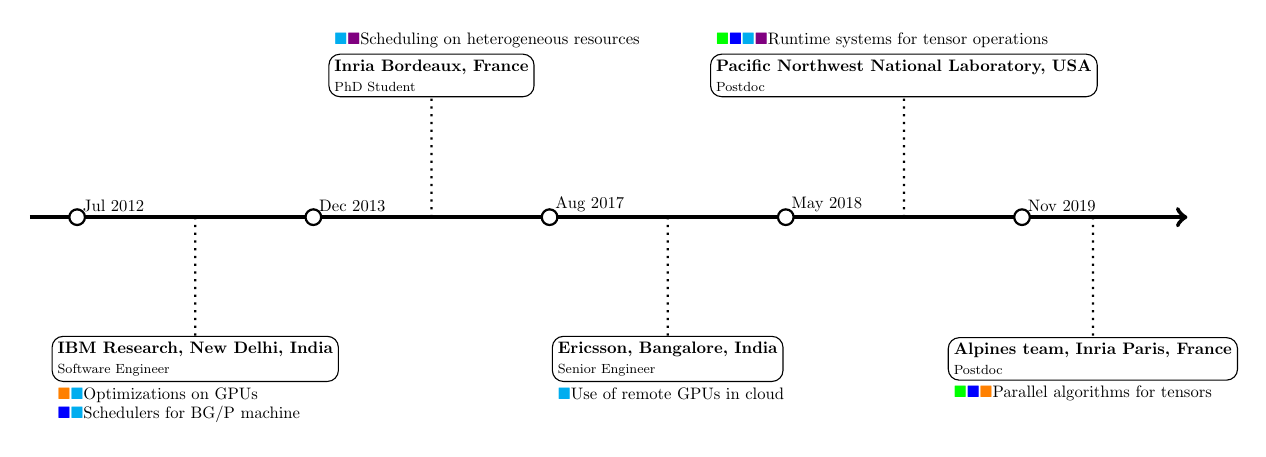
\begin{tikzpicture}[scale=0.6, every node/.style={transform shape}]

	\tikzstyle{taskc}=[circle, thick, draw=black, minimum size=2mm, fill=white]
	
%%	\tikzstyle{taskr}=[rectangle, rounded corners, draw=black, minimum size=2mm, fill=none]
	\tikzstyle{taskr}=[draw=black, rounded corners, minimum height=8mm, minimum width=8mm, fill=none, text=black]
	
	\draw [->, ultra thick](-1,0) -- (23.5, 0);
	\node (t0) at (0,0) [taskc] {};
	\node [above right] at (t0) {Jul 2012};
	
	\node (t1) at (5,0) [taskc] {};
	\node [above right] at (t1) {Dec 2013};
	\node (t2) at (10,0) [taskc] {};
	\node [above right] at (t2) {Aug 2017};
	\node (t3) at (15,0) [taskc] {};
	\node [above right] at (t3) {May 2018};
	\node (t4) at (20,0) [taskc] {};
	\node [above right] at (t4) {Nov 2019};
	

	\node (ibmnode) at (2.5, -3) [taskr, align=left] {\textbf{IBM Research, New Delhi, India}\\{\footnotesize Software Engineer}};
	\node [below, align=left, anchor=north west] at (ibmnode.south west) {\mysymbole \mysymbolc Optimizations on GPUs\\ \mysymbolb \mysymbolc Schedulers for BG/P machine};
	
	\draw [dotted, thick] (2.5, 0) -- (ibmnode);

	\node (phdnode) at (7.5, 3) [taskr, align=left] {\textbf{Inria Bordeaux, France}\\{\footnotesize PhD Student}};
	\node [above, align=left, anchor=south west] at (phdnode.north west) {\mysymbolc \mysymbold Scheduling on heterogeneous resources};
	
	\draw [dotted, thick] (7.5, 0) -- (phdnode);
	
	\node (ericssonnode) at (12.5, -3) [taskr, align=left] {\textbf{Ericsson, Bangalore, India}\\{\footnotesize Senior Engineer}};
	\node [below, align=left, anchor=north west] at (ericssonnode.south west) {\mysymbolc Use of remote GPUs in cloud};
	
	\draw [dotted, thick] (12.5, 0) -- (ericssonnode);
	
	\node (pnnlnode) at (17.5, 3) [taskr, align=left] {\textbf{Pacific Northwest National Laboratory, USA}\\{\footnotesize Postdoc}};
	\node [above, align=left, anchor=south west] at (pnnlnode.north west) {\mysymbola \mysymbolb \mysymbolc \mysymbold Runtime systems for tensor operations};
	
	\draw [dotted, thick] (17.5, 0) -- (pnnlnode);
	
	\node (alpinesnode) at (21.5, -3) [taskr, align=left] {\textbf{Alpines team, Inria Paris, France}\\{\footnotesize Postdoc}};
	\node [below, align=left, anchor=north west] at (alpinesnode.south west) {\mysymbola \mysymbolb \mysymbole Parallel algorithms for tensors};
	
	\draw [dotted, thick] (21.5, 0) -- (alpinesnode);
\end{tikzpicture}
}
\end{frame}





%%\begin{tikzpicture}[scale=0.625, every node/.style={transform shape}]
%%%%\tikzstyle{taskmemory}=[draw=black, minimum height=18mm, minimum width=18mm, fill=blue!40, text=black]
%%\tikzstyle{taskcompute}=[draw=black, minimum height=16mm, minimum width=16mm, fill=none, text=black, below]
%%
%%\node (t0) at (0,0) [taskcompute] {}; 
%%\node (t1) at (4,0) [taskcompute] {};
%%\node (t2) at (4,4) [taskcompute] {};
%%\node (t3) at (0,4) [taskcompute] {};
%%
%%\draw [<->, line width=4, orange] (t0) -- (t1);
%%\draw [<->, line width=4, orange] (t1) -- (t2);
%%\draw [<->, line width=4, orange] (t2) -- (t3);
%%\draw [<->, line width=4, orange] (t3) -- (t0);
%%
%%\node (td0)  at (t0.south) [above, scale=0.5] {$DRAM$};
%%\node (td1) [above, scale=0.5] at (t1.south) {$DRAM$};
%%\node (td2) [above, scale=0.5] at (t2.south) {$DRAM$};
%%\node (td3) [above, scale=0.5] at (t3.south) {$DRAM$};
%%
%%\node [above] at (td0.north) {$CPU$};
%%\node [above] at (td1.north) {$CPU$};
%%\node [above] at (td2.north) {$CPU$};
%%\node [above] at (td3.north) {$CPU$};
%%
%%%%\node [below] at (tm.south) {Memory Unit $M$};
%%%%\node [above] at (tc.north) {Compute Unit $C$};
%%%%
%%%%\node [taskmemory, minimum height=6mm, minimum width=12mm, anchor=south] at (tc.south) {}; 
%%\end{tikzpicture}


%%\begin{tikzpicture}[shorten >=1pt,node distance=5cm,on grid,auto] 
%%
%%\node[state,initial] (q_0) {$q_0$}; 
%%\path[->] (q_0) edge[loop above] node[text width=1cm,align=center] {0,1,2\\3,4,5} (q_0); 
%%
%%\end{tikzpicture}
%%	\begin{itemize}
%%		
%%		\item 11/2019 -- Current, Postdoc, Alpines team, Inria Paris, France
%%		\begin{itemize}
%%			\item \mysymbola \mysymbolb \mysymbole Parallel algorithms for high dimensional tensor computations
%%		\end{itemize}
%%		
%%		\item 05/2018 -- 10/2019, Postdoc, Pacific Northwest National Laboratory, USA
%%		\begin{itemize}
%%			\item \mysymbola \mysymbolb \mysymbolc \mysymbold Runtime systems for molecular simulations
%%		\end{itemize}
%%		
%%		\item 08/2017 -- 02/2018, Senior Engineer, Ericsson, Bangalore, India
%%		\begin{itemize}
%%			\item\mysymbolc Use of remote GPUs in cloud
%%		\end{itemize}
%%		
%%		
%%		\item 12/2013 -- 06/2017, PhD Student, University of Bordeaux \& Inria Bordeaux, France
%%		\begin{itemize}
%%			\item \mysymbolc \mysymbold Scheduling of dense linear algebra kernels on heterogeneous resources
%%		\end{itemize}
%%		
%%		
%%		\item 07/2012 -- 11/2013, Software Engineer, IBM Research, New Delhi, India
%%		\begin{itemize}
%%			\item \mysymbole \mysymbolc Performance optimizations of seismic algorithms on GPU, \mysymbolc Schedulers for BG/P machine
%%		\end{itemize}
%%		
%%		\item 08/2010 -- 06/2012, Master Student, Indian Institute of Science, Bangalore, India
%%		\begin{itemize}
%%			\item \mysymbolb Automatic parallelization of programs with linked-lists 
%%		\end{itemize}
%%		
%%	\end{itemize}



\part[Past/Ongoing Work]{Past/Ongoing Work}

%%\begin{frame}{Collaborators}
%%This is joint work with ...
%%\begin{itemize}
%%	\item Laura Grigori -- Inria Paris, France
%%	\item Grey Ballard -- Wake Forest University, USA
%%	\item Hussam Al Daas -- STFC Rutherford Appleton Laboratory, UK
%%	\item Olivier Beaumont -- Inria Bordeaux, France
%%	\item Sriram Krishnamoorthy -- Pacific Northwest National Laboratory, USA
%%	\item Marcin Zalewski -- Nvidia, USA
%%	\item Lionel Eyraud-Dubois -- Inria Bordeaux, France
%%	\item Samuel Thibault -- Inria Bordeaux, France
%%	\item Emmanuel Agullo -- Inria Bordeaux, France
%%\end{itemize}
%%\end{frame}


%%\begin{frame}
%%\frametitle{Overview} % Table of contents slide, comment this block out to remove it
%%\tableofcontents[part=1] % Throughout your presentation, if you choose to use \section{} and \subsection{} commands, these will automatically be printed on this slide as an overview of your presentation
%%\end{frame}


%%%%\begin{frame}
%%%%\frametitle{Part1: Past/Ongoing Work} % Table of contents slide, comment this block out to remove it
%%%%\tableofcontents[part=1] % Throughout your presentation, if you choose to use \section{} and \subsection{} commands, these will automatically be printed on this slide as an overview of your presentation
%%%%\end{frame}


%%\section{Tensors and their Popular Decompositions}

%%\begin{frame}{Tensors: Multidimensional Arrays}
%%\begin{tabular}{ccc}
%%	Dimension & Name &\\
%%	%%\begin{tikzpicture}[scale=0.625, every node/.style={transform shape}]
%%	%%\tikzstyle{taskr}=[draw=black, minimum height=1mm, minimum width=12mm, anchor=south west, fill=pastelgreen, text=black]
%%	%%			\node (t01) at (0,0) [taskr]{};
%%	%%\end{tikzpicture}
%%	%%\begin{tikzpicture}
%%	%%\pgfmathsetmacro{\cubex}{5}
%%	%%\pgfmathsetmacro{\cubey}{1}
%%	%%\pgfmathsetmacro{\cubez}{3}
%%	%%\draw[red,fill=yellow] (0,0,0) -- ++(-\cubex,0,0) -- ++(0,-\cubey,0) -- ++(\cubex,0,0) -- cycle;
%%	%%\draw[red,fill=yellow] (0,0,0) -- ++(0,0,-\cubez) -- ++(0,-\cubey,0) -- ++(0,0,\cubez) -- cycle;
%%	%%\draw[red,fill=yellow] (0,0,0) -- ++(-\cubex,0,0) -- ++(0,0,-\cubez) -- ++(\cubex,0,0) -- cycle;
%%	%%\end{tikzpicture}
%%	%%$0$ & Scalar & \\
%%	$1$ & Vector & \begin{tikzpicture}[scale=0.25, every node/.style={transform shape}]
%%	\pgfmathsetmacro{\rectx}{4}
%%	\pgfmathsetmacro{\recty}{0.5}
%%	\draw[blue,fill=pastelgreen] (0,0) -- ++(-\rectx,0) -- ++(0,\recty) -- ++(\rectx, 0) -- cycle;
%%	\end{tikzpicture} \\
%%	&&\\
%%	$2$ & Matrix & \begin{tikzpicture}[scale=0.25, every node/.style={transform shape}]
%%	\pgfmathsetmacro{\rectx}{4}
%%	\pgfmathsetmacro{\recty}{4}
%%	\draw[blue,fill=pastelgreen] (0,0) -- ++(-\rectx,0) -- ++(0,\recty) -- ++(\rectx, 0) -- cycle;
%%	%%\addvmargin{4};
%%	\end{tikzpicture}\\
%%	&&\\
%%	$3$ & $3$-dimensional tensor & \begin{tikzpicture}[scale=0.25, every node/.style={transform shape}]
%%	\pgfmathsetmacro{\cubex}{4}
%%	\pgfmathsetmacro{\cubey}{4}
%%	\pgfmathsetmacro{\cubez}{4}
%%	\draw[blue,fill=pastelgreen] (0,0,0) -- ++(-\cubex,0,0) -- ++(0,-\cubey,0) -- ++(\cubex,0,0) -- cycle;
%%	\draw[blue,fill=pastelgreen] (0,0,0) -- ++(0,0,-\cubez) -- ++(0,-\cubey,0) -- ++(0,0,\cubez) -- cycle;
%%	\draw[blue,fill=pastelgreen] (0,0,0) -- ++(-\cubex,0,0) -- ++(0,0,-\cubez) -- ++(\cubex,0,0) -- cycle;
%%	\end{tikzpicture}\\
%%	&&\\
%%	$4$ & $4$-dimensional tensor & 
%%	\begin{tikzpicture}[scale=0.25, every node/.style={transform shape}]
%%	\pgfmathsetmacro{\cubex}{4}
%%	\pgfmathsetmacro{\cubey}{4}
%%	\pgfmathsetmacro{\cubez}{4}
%%	\draw[blue,fill=pastelgreen] (0,0,0) -- ++(-\cubex,0,0) -- ++(0,-\cubey,0) -- ++(\cubex,0,0) -- cycle;
%%	\draw[blue,fill=pastelgreen] (0,0,0) -- ++(0,0,-\cubez) -- ++(0,-\cubey,0) -- ++(0,0,\cubez) -- cycle;
%%	\draw[blue,fill=pastelgreen] (0,0,0) -- ++(-\cubex,0,0) -- ++(0,0,-\cubez) -- ++(\cubex,0,0) -- cycle;
%%	
%%	\draw[blue,fill=pastelgreen] (\cubex +2,0,0) -- ++(-\cubex,0,0) -- ++(0,-\cubey,0) -- ++(\cubex,0,0) -- cycle;
%%	\draw[blue,fill=pastelgreen] (\cubex +2,0,0) -- ++(0,0,-\cubez) -- ++(0,-\cubey,0) -- ++(0,0,\cubez) -- cycle;
%%	\draw[blue,fill=pastelgreen] (\cubex +2,0,0) -- ++(-\cubex,0,0) -- ++(0,0,-\cubez) -- ++(\cubex,0,0) -- cycle;
%%	
%%	\draw[blue,fill=pastelgreen] (\cubex +2 + \cubex +2,0,0) -- ++(-\cubex,0,0) -- ++(0,-\cubey,0) -- ++(\cubex,0,0) -- cycle;
%%	\draw[blue,fill=pastelgreen] (\cubex +2 + \cubex +2,0,0) -- ++(0,0,-\cubez) -- ++(0,-\cubey,0) -- ++(0,0,\cubez) -- cycle;
%%	\draw[blue,fill=pastelgreen] (\cubex +2 + \cubex +2,0,0) -- ++(-\cubex,0,0) -- ++(0,0,-\cubez) -- ++(\cubex,0,0) -- cycle;
%%	
%%	\draw[blue, fill=none] (-\cubex -1, 2.5, 0) -- ++(0, -\cubey -3.5, 0) -- ++(\cubex +2 + \cubex +2 + \cubex + \cubex,0,0) -- ++(0, \cubey +3.5, 0) -- cycle; 
%%	\end{tikzpicture}
%%\end{tabular}
%%
%%\end{frame}
%%
%%%------------------------------------------------
%%
%%
%%\begin{frame}{test}
%%\begin{tikzpicture}[scale=0.125, every node/.style={transform shape}]
%%\pgfmathsetmacro{\rectx}{4}
%%\pgfmathsetmacro{\recty}{0.5}
%%\draw[blue,fill=pastelgreen] (0,0) -- node [below, scale=6, black] {Vector}++(-\rectx,0) -- ++(0,\recty) -- ++(\rectx, 0) -- cycle;
%%\end{tikzpicture}$\quad$
%%\begin{tikzpicture}[scale=0.125, every node/.style={transform shape}]
%%\pgfmathsetmacro{\rectx}{4}
%%\pgfmathsetmacro{\recty}{4}
%%\draw[blue,fill=pastelgreen] (0,0) -- node [below, scale=6, black] {Matrix}++(-\rectx,0) -- ++(0,\recty) -- ++(\rectx, 0) -- cycle;
%%%%\addvmargin{4};
%%\end{tikzpicture}$\quad$
%%\begin{tikzpicture}[scale=0.125, every node/.style={transform shape}]
%%\pgfmathsetmacro{\cubex}{4}
%%\pgfmathsetmacro{\cubey}{4}
%%\pgfmathsetmacro{\cubez}{4}
%%\draw[blue,fill=pastelgreen] (0,0,0) -- ++(-\cubex,0,0) -- ++(0,-\cubey,0) --node [below, scale=6, black] {3-dimensional tensor} ++(\cubex,0,0) -- cycle;
%%\draw[blue,fill=pastelgreen] (0,0,0) -- ++(0,0,-\cubez) -- ++(0,-\cubey,0) -- ++(0,0,\cubez) -- cycle;
%%\draw[blue,fill=pastelgreen] (0,0,0) -- ++(-\cubex,0,0) -- ++(0,0,-\cubez) -- ++(\cubex,0,0) -- cycle;
%%\end{tikzpicture}$\quad$
%%	\begin{tikzpicture}[scale=0.125, every node/.style={transform shape}]
%%\pgfmathsetmacro{\cubex}{4}
%%\pgfmathsetmacro{\cubey}{4}
%%\pgfmathsetmacro{\cubez}{4}
%%\draw[blue,fill=pastelgreen] (0,0,0) -- ++(-\cubex,0,0) -- ++(0,-\cubey,0) -- ++(\cubex,0,0) -- cycle;
%%\draw[blue,fill=pastelgreen] (0,0,0) -- ++(0,0,-\cubez) -- ++(0,-\cubey,0) -- ++(0,0,\cubez) -- cycle;
%%\draw[blue,fill=pastelgreen] (0,0,0) -- ++(-\cubex,0,0) -- ++(0,0,-\cubez) -- ++(\cubex,0,0) -- cycle;
%%
%%\draw[blue,fill=pastelgreen] (\cubex +2,0,0) -- ++(-\cubex,0,0) -- ++(0,-\cubey,0) -- ++(\cubex,0,0) -- cycle;
%%\draw[blue,fill=pastelgreen] (\cubex +2,0,0) -- ++(0,0,-\cubez) -- ++(0,-\cubey,0) -- ++(0,0,\cubez) -- cycle;
%%\draw[blue,fill=pastelgreen] (\cubex +2,0,0) -- ++(-\cubex,0,0) -- ++(0,0,-\cubez) -- ++(\cubex,0,0) -- cycle;
%%
%%\draw[blue,fill=pastelgreen] (\cubex +2 + \cubex +2,0,0) -- ++(-\cubex,0,0) -- ++(0,-\cubey,0) -- ++(\cubex,0,0) -- cycle;
%%\draw[blue,fill=pastelgreen] (\cubex +2 + \cubex +2,0,0) -- ++(0,0,-\cubez) -- ++(0,-\cubey,0) -- ++(0,0,\cubez) -- cycle;
%%\draw[blue,fill=pastelgreen] (\cubex +2 + \cubex +2,0,0) -- ++(-\cubex,0,0) -- ++(0,0,-\cubez) -- ++(\cubex,0,0) -- cycle;
%%
%%\draw[blue, fill=none] (-\cubex -1, 2.5, 0) -- ++(0, -\cubey -3.5, 0) --node [below, scale=6, black] {4-dimensional tensor} ++(\cubex +2 + \cubex +2 + \cubex + \cubex,0,0) -- ++(0, \cubey +3.5, 0) -- cycle; 
%%
%%%%\node [scale=2] at (0, -8) {$hello$};
%%\end{tikzpicture}
%%
%%\end{frame}

\begin{frame}{Tensors are used in Several Domains}
\begin{minipage}{0.575\linewidth}
\begin{itemize}
	\item \textbf{Neuroscience}: Neuron $\times$ Time $\times$ Trial
	\item \textbf{Transportation}: Pickup $\times$ Dropoff $\times$ Time
	\item \textbf{Media}: User x Movie x Time 
	\item \textbf{Ecommerce}: User x Product x Time
\end{itemize}
\end{minipage}
\begin{minipage}{0.4\linewidth}
	\begin{center}
	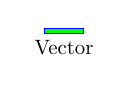
\begin{tikzpicture}[scale=0.125, every node/.style={transform shape}]
	\pgfmathsetmacro{\rectx}{4}
	\pgfmathsetmacro{\recty}{0.5}
	\draw[blue,fill=pastelgreen] (0,0) -- node [below, scale=6, black] {Vector}++(-\rectx,0) -- ++(0,\recty) -- ++(\rectx, 0) -- cycle;
	\end{tikzpicture}$\quad$
	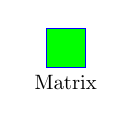
\begin{tikzpicture}[scale=0.125, every node/.style={transform shape}]
	\pgfmathsetmacro{\rectx}{4}
	\pgfmathsetmacro{\recty}{4}
	\draw[blue,fill=pastelgreen] (0,0) -- node [below, scale=6, black] {Matrix}++(-\rectx,0) -- ++(0,\recty) -- ++(\rectx, 0) -- cycle;
	%%\addvmargin{4};
	\end{tikzpicture}$\ $
	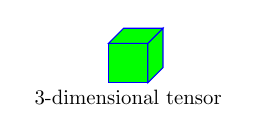
\begin{tikzpicture}[scale=0.125, every node/.style={transform shape}]
	\pgfmathsetmacro{\cubex}{4}
	\pgfmathsetmacro{\cubey}{4}
	\pgfmathsetmacro{\cubez}{4}
	\draw[blue,fill=pastelgreen] (0,0,0) -- ++(-\cubex,0,0) -- ++(0,-\cubey,0) --node [below, scale=6, black] {3-dimensional tensor} ++(\cubex,0,0) -- cycle;
	\draw[blue,fill=pastelgreen] (0,0,0) -- ++(0,0,-\cubez) -- ++(0,-\cubey,0) -- ++(0,0,\cubez) -- cycle;
	\draw[blue,fill=pastelgreen] (0,0,0) -- ++(-\cubex,0,0) -- ++(0,0,-\cubez) -- ++(\cubex,0,0) -- cycle;
	\end{tikzpicture}
	\end{center}
\begin{center}	
	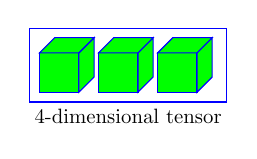
\begin{tikzpicture}[scale=0.125, every node/.style={transform shape}]
	\pgfmathsetmacro{\cubex}{4}
	\pgfmathsetmacro{\cubey}{4}
	\pgfmathsetmacro{\cubez}{4}
	\draw[blue,fill=pastelgreen] (0,0,0) -- ++(-\cubex,0,0) -- ++(0,-\cubey,0) -- ++(\cubex,0,0) -- cycle;
	\draw[blue,fill=pastelgreen] (0,0,0) -- ++(0,0,-\cubez) -- ++(0,-\cubey,0) -- ++(0,0,\cubez) -- cycle;
	\draw[blue,fill=pastelgreen] (0,0,0) -- ++(-\cubex,0,0) -- ++(0,0,-\cubez) -- ++(\cubex,0,0) -- cycle;
	
	\draw[blue,fill=pastelgreen] (\cubex +2,0,0) -- ++(-\cubex,0,0) -- ++(0,-\cubey,0) -- ++(\cubex,0,0) -- cycle;
	\draw[blue,fill=pastelgreen] (\cubex +2,0,0) -- ++(0,0,-\cubez) -- ++(0,-\cubey,0) -- ++(0,0,\cubez) -- cycle;
	\draw[blue,fill=pastelgreen] (\cubex +2,0,0) -- ++(-\cubex,0,0) -- ++(0,0,-\cubez) -- ++(\cubex,0,0) -- cycle;
	
	\draw[blue,fill=pastelgreen] (\cubex +2 + \cubex +2,0,0) -- ++(-\cubex,0,0) -- ++(0,-\cubey,0) -- ++(\cubex,0,0) -- cycle;
	\draw[blue,fill=pastelgreen] (\cubex +2 + \cubex +2,0,0) -- ++(0,0,-\cubez) -- ++(0,-\cubey,0) -- ++(0,0,\cubez) -- cycle;
	\draw[blue,fill=pastelgreen] (\cubex +2 + \cubex +2,0,0) -- ++(-\cubex,0,0) -- ++(0,0,-\cubez) -- ++(\cubex,0,0) -- cycle;
	
	\draw[blue, fill=none] (-\cubex -1, 2.5, 0) -- ++(0, -\cubey -3.5, 0) --node [below, scale=6, black] {4-dimensional tensor} ++(\cubex +2 + \cubex +2 + \cubex + \cubex,0,0) -- ++(0, \cubey +3.5, 0) -- cycle; 
	
	%%\node [scale=2] at (0, -8) {$hello$};
	\end{tikzpicture}
\end{center}
\end{minipage}
\vspace*{-0.2cm}
\begin{itemize}
	\item \textbf{Cyber-Traffic}: IP x IP x Port x Time
	\item \textbf{Social-Network}: Person x Person x Time x Interaction-Type
\end{itemize}
\begin{block}{High Dimensional Tensors}
\begin{itemize}
	\item \textbf{Neural Network}: \begin{center}\vspace*{-0.35cm}
	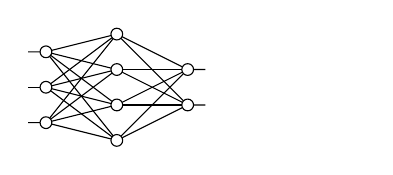
\begin{tikzpicture}[scale=0.45, every node/.style={transform shape}]
	\tikzstyle{taskc}=[circle, draw=black, minimum size=2mm, fill=none]
	
	\node (t00) at (0,1) [taskc] {};
	\node (t01) at (0,0) [taskc] {};
	\node (t02) at (0,-1) [taskc] {};
	
	\draw (-0.5,1) -- (t00);
	\draw (-0.5,0) -- (t01);
	\draw (-0.5,-1) -- (t02);
	
	\node (t10) at (2,1.5) [taskc] {};
	\node (t11) at (2,0.5) [taskc] {};
	\node (t12) at (2,-0.5) [taskc] {};
	\node (t13) at (2,-1.5) [taskc] {};
	
	\draw (t00) -- (t10);
	\draw (t00) -- (t11);
	\draw (t00) -- (t12);
	\draw (t00) -- (t13);
	
	\draw (t01) -- (t10);
	\draw (t01) -- (t11);
	\draw (t01) -- (t12);
	\draw (t01) -- (t13);
	
	\draw (t02) -- (t10);
	\draw (t02) -- (t11);
	\draw (t02) -- (t12);
	\draw (t02) -- (t13);
	
	\node (t20) at (4,0.5) [taskc] {};
	\node (t21) at (4,-0.5) [taskc] {};
	
	\draw (t10) -- (t20);
	\draw (t10) -- (t21);
	
	\draw (t11) -- (t20);
	\draw (t11) -- (t21);
	
	\draw (t12) -- (t20);
	\draw (t12) -- (t21);
	
	\draw (t13) -- (t20);
	\draw (t13) -- (t21);
	
	\draw (t20) -- (4.5, 0.5);
	\draw (t21) -- (4.5, -0.5);
%%	\node (t01) at (0,0) [taskc]{};
%%	\draw (t01) -- (1,0);
%%	\draw (t01) -- (-1,0);
	\path (6.8, 0) -- (9.0,0);
	\end{tikzpicture} 	
%%%%	\begin{tikzpicture}[scale=0.45, every node/.style={transform shape}]
%%%%	\tikzstyle{taskc}=[ellipse, draw=black, minimum width=40mm, minimum height=15mm, fill=\tensorcolor]
%%%%	\node (t0) at (0,0) [taskc] {};
%%%%	
%%%%	\draw(0, -1.5) -- (t0);
%%%%	\draw(-0.5, -1.5) -- (-0.5, 0);
%%%%	\draw(0.5, -1.5) -- (0.5, 0);
%%%%	
%%%%	\draw(-0.25,0) -- (-0.25,1.5);
%%%%	\draw(0.25,0) -- (0.25,1.5);
%%%%	
%%%%	
%%%%	\node (t0) at (0,0) [taskc] {};
%%%%	\end{tikzpicture}
\end{center}
%%	\includegraphics[scale=0.02]{./tmp/neuralNetwork.jpg}
	\item \textbf{Molecular Simulation}: To represent wave functions
	\item \textbf{Quantum Computing}: To represent qubit states

\end{itemize}
\end{block}
\end{frame}



\begin{frame}{Tensor Computations}

{\small
\begin{itemize}
%%	\item Tensors are used in several domains
%%	\begin{itemize}
%%		\item Quantum molecular dynamics, signal processing, data mining, neurosciences, computer vision, psychometrics, chemometrics, ...
%%	\end{itemize}
%%	\vfill
	\item Memory and computation requirements are exponential in the number of dimensions
	\begin{itemize}
		\item A simulation involving just $100$ spatial orbitals manipulates a huge tensor with $4^{100}$ elements

	\end{itemize}
	\vfill
	\item People work with low dimensional structure (decomposition) of the tensors
	\begin{itemize}
		\item A tensor is represented with smaller objects
%%		\item Useful to find patterns in massive data
		\item Improves memory and computation requirements
	\end{itemize}
	\vfill
%%	\item Singular value decomposition (SVD) provides the most accurate low rank approximations for matrices
%%	\vfill
%%	\begin{itemize}
%%		\item Most tensor decompositions are based on SVD of matricized tensors
%%	\end{itemize} 
%%	\vfill
%%%%	\item Limited work on parallelization of tensor algorithms
%%%%	
%%%%	\vfill
	\item Most tensor decompositions rely on Singular Value Decomposition (SVD) of matrices
%%	\item Singular Value Decomposition (SVD) provides the most accurate low rank approximations of matrices
	\begin{itemize}
		%%	\item It decomposes a matrix $A$ $\in$ $\mathbb{R}^{m \times n}$ to the form $U\Sigma V^T$
		%%	\begin{itemize}
		%%		\item $U$ is an $m\times m$ orthogonal matrix
		%%		\item $V$ is an $n\times n$ orthogonal matrix
		%%		\item $\Sigma$ is an $m\times n$ rectangular diagonal matrix
		%%	\end{itemize}
		\item SVD represents a matrix as the sum of rank one matrices, $A= U\Sigma V^T= \sum_i\Sigma(i;i)U_i V_i^T$
		%%%%	\begin{itemize}
		%%%%%%		\item $A= \sum_i \Sigma(i;i)U_i V_i^T$
		%%%%		\item Minimum number of rank one matrices required in the sum is called the rank of the matrix
		%%%%	\end{itemize}
		\begin{center}
			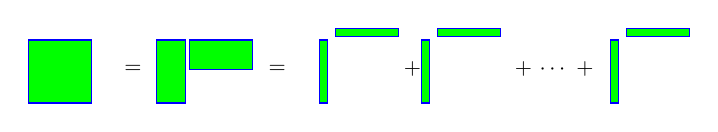
\begin{tikzpicture}[scale=0.2, every node/.style={transform shape}]
			\pgfmathsetmacro{\cubex}{4}
			\pgfmathsetmacro{\cubey}{4}
			\pgfmathsetmacro{\cubez}{4}
			\draw[blue,fill=pastelgreen] (0,0,0) -- ++(-\cubex,0,0) -- ++(0,-\cubey,0) -- ++(\cubex,0,0) -- cycle;
			%%\draw[blue,fill=pastelgreen] (0,0,0) -- ++(0,0,-\cubez) -- ++(0,-\cubey,0) -- ++(0,0,\cubez) -- cycle;
			%%\draw[blue,fill=pastelgreen] (0,0,0) -- ++(-\cubex,0,0) -- ++(0,0,-\cubez) -- ++(\cubex,0,0) -- cycle;
			
			\node[draw=none, text=black, scale=4] at (1.5,-3,-3) {$=$};
			
			\draw[blue,fill=pastelgreen] (6,0,0) -- ++(-\cubex+2.15,0,0) -- ++(0,-\cubey,0) -- ++(\cubex-2.15,0,0) -- cycle;
			
			\draw[blue,fill=pastelgreen] (10.25,0,0) -- ++(-\cubex,0,0) -- ++(0,-\cubey+2.15,0) -- ++(\cubex,0,0) -- cycle;
			
			\node[draw=none, text=black, scale=4] at (10.65,-3,-3) {$=$};
			
			\pgfmathsetmacro{\smallwidth}{0.5}
			\draw[blue,fill=pastelgreen] (9+\cubex+2,0,0) -- ++(-\smallwidth,0,0) -- ++(0,-\cubey,0) -- ++(\smallwidth,0,0) -- cycle;
			\draw[blue,fill=pastelgreen] (9+\cubex+2 +\cubex + 0.5,0.75,0) -- ++(-\cubex,0,0) -- ++(0,-\smallwidth,0) -- ++(\cubex,0,0) -- cycle;
			%%\draw[blue,fill=pastelgreen] (\cubex+2,0.5,0) -- ++(-\smallwidth,0,0) -- ++(0,0,-\cubez) -- ++(\smallwidth,0,0) -- cycle;
			
			\node[draw=none, text=black, scale=4] at (9+2+\cubex+4.25,-3,-3) {$+$};
			
			\draw[blue,fill=pastelgreen] (9+\cubex+2.5 + \cubex+2,0,0) -- ++(-\smallwidth,0,0) -- ++(0,-\cubey,0) -- ++(\smallwidth,0,0) -- cycle;
			\draw[blue,fill=pastelgreen] (9+\cubex+2.5+\cubex+2 +\cubex + 0.5,0.75,0) -- ++(-\cubex,0,0) -- ++(0,-\smallwidth,0) -- ++(\cubex,0,0) -- cycle;
			%%\draw[blue,fill=pastelgreen] (\cubex+2.5+\cubex+2,0.5,0) -- ++(-\smallwidth,0,0) -- ++(0,0,-\cubez) -- ++(\smallwidth,0,0) -- cycle;
			
			\node[draw=none, text=black, scale=4] at (9+2+\cubex+5 + \cubex+ 4.25, -3,-3) {$+$ $\cdots$ $+$};
			
			\draw[blue,fill=pastelgreen] (9+12 + \cubex+2.5 + \cubex+2,0,0) -- ++(-\smallwidth,0,0) -- ++(0,-\cubey,0) -- ++(\smallwidth,0,0) -- cycle;
			\draw[blue,fill=pastelgreen] (9+12+\cubex+2.5+\cubex+2 +\cubex + 0.5,0.75,0) -- ++(-\cubex,0,0) -- ++(0,-\smallwidth,0) -- ++(\cubex,0,0) -- cycle;
			%%\draw[blue,fill=pastelgreen] (12 + \cubex+2.5+\cubex+2,0.5,0) -- ++(-\smallwidth,0,0) -- ++(0,0,-\cubez) -- ++(\smallwidth,0,0) -- cycle;
			\end{tikzpicture}$\qquad\qquad\qquad\qquad$
		\end{center}
	\end{itemize}
	
	%%    \begin{itemize}
	%%    	\item Matricized Tensor Times Khatri Rao Product (MTTKRP), tensor contraction
	%%    \end{itemize}
\end{itemize}
}
\end{frame}

%%\begin{frame}{Use of Tensors}
%%content...
%%\end{frame}
\begin{frame}{Popular Tensor Decompositions (Higher Order Generalization of SVD)}

{\small
%%%%\begin{itemize}
%%%%%%	\item It decomposes a matrix $A$ $\in$ $\mathbb{R}^{m \times n}$ to the form $U\Sigma V^T$
%%%%%%	\begin{itemize}
%%%%%%		\item $U$ is an $m\times m$ orthogonal matrix
%%%%%%		\item $V$ is an $n\times n$ orthogonal matrix
%%%%%%		\item $\Sigma$ is an $m\times n$ rectangular diagonal matrix
%%%%%%	\end{itemize}
%%%%	\item SVD represents a matrix as the sum of rank one matrices, $A= U\Sigma V^T= \Sigma(i;i)U_i V_i^T$
%%%%%%%%	\begin{itemize}
%%%%%%%%%%		\item $A= \sum_i \Sigma(i;i)U_i V_i^T$
%%%%%%%%		\item Minimum number of rank one matrices required in the sum is called the rank of the matrix
%%%%%%%%	\end{itemize}
%%%%\begin{center}
%%%%	\begin{tikzpicture}[scale=0.2, every node/.style={transform shape}]
%%%%	\pgfmathsetmacro{\cubex}{4}
%%%%	\pgfmathsetmacro{\cubey}{4}
%%%%	\pgfmathsetmacro{\cubez}{4}
%%%%	\draw[blue,fill=pastelgreen] (0,0,0) -- ++(-\cubex,0,0) -- ++(0,-\cubey,0) -- ++(\cubex,0,0) -- cycle;
%%%%	%%\draw[blue,fill=pastelgreen] (0,0,0) -- ++(0,0,-\cubez) -- ++(0,-\cubey,0) -- ++(0,0,\cubez) -- cycle;
%%%%	%%\draw[blue,fill=pastelgreen] (0,0,0) -- ++(-\cubex,0,0) -- ++(0,0,-\cubez) -- ++(\cubex,0,0) -- cycle;
%%%%	
%%%%	\node[draw=none, text=black, scale=4] at (2,-3,-3) {$=$};
%%%%	\pgfmathsetmacro{\smallwidth}{0.5}
%%%%	\draw[blue,fill=pastelgreen] (\cubex+2,0,0) -- ++(-\smallwidth,0,0) -- ++(0,-\cubey,0) -- ++(\smallwidth,0,0) -- cycle;
%%%%	\draw[blue,fill=pastelgreen] (\cubex+2 +\cubex + 0.5,0.75,0) -- ++(-\cubex,0,0) -- ++(0,-\smallwidth,0) -- ++(\cubex,0,0) -- cycle;
%%%%	%%\draw[blue,fill=pastelgreen] (\cubex+2,0.5,0) -- ++(-\smallwidth,0,0) -- ++(0,0,-\cubez) -- ++(\smallwidth,0,0) -- cycle;
%%%%	
%%%%	\node[draw=none, text=black, scale=4] at (2+\cubex+4.25,-3,-3) {$+$};
%%%%	
%%%%	\draw[blue,fill=pastelgreen] (\cubex+2.5 + \cubex+2,0,0) -- ++(-\smallwidth,0,0) -- ++(0,-\cubey,0) -- ++(\smallwidth,0,0) -- cycle;
%%%%	\draw[blue,fill=pastelgreen] (\cubex+2.5+\cubex+2 +\cubex + 0.5,0.75,0) -- ++(-\cubex,0,0) -- ++(0,-\smallwidth,0) -- ++(\cubex,0,0) -- cycle;
%%%%	%%\draw[blue,fill=pastelgreen] (\cubex+2.5+\cubex+2,0.5,0) -- ++(-\smallwidth,0,0) -- ++(0,0,-\cubez) -- ++(\smallwidth,0,0) -- cycle;
%%%%	
%%%%	\node[draw=none, text=black, scale=4] at (2+\cubex+5 + \cubex+ 4.25, -3,-3) {$+$ $\cdots$ $+$};
%%%%	
%%%%	\draw[blue,fill=pastelgreen] (12 + \cubex+2.5 + \cubex+2,0,0) -- ++(-\smallwidth,0,0) -- ++(0,-\cubey,0) -- ++(\smallwidth,0,0) -- cycle;
%%%%	\draw[blue,fill=pastelgreen] (12+\cubex+2.5+\cubex+2 +\cubex + 0.5,0.75,0) -- ++(-\cubex,0,0) -- ++(0,-\smallwidth,0) -- ++(\cubex,0,0) -- cycle;
%%%%	%%\draw[blue,fill=pastelgreen] (12 + \cubex+2.5+\cubex+2,0.5,0) -- ++(-\smallwidth,0,0) -- ++(0,0,-\cubez) -- ++(\smallwidth,0,0) -- cycle;
%%%%	\end{tikzpicture}
%%%%\end{center}
%%%%\end{itemize}
%%%%\vspace*{-0.35cm}
%%\begin{block}{}
\vspace*{-0.25cm}
\begin{itemize}
	\item Canonical decomposition (Also known as Canonical Polyadic or CANDECOMP/PARAFAC)
	\begin{center}
		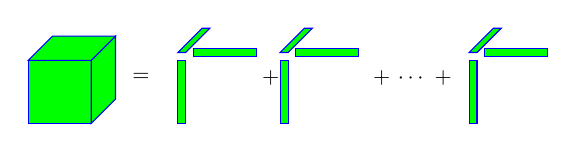
\begin{tikzpicture}[scale=0.2, every node/.style={transform shape}]
		\pgfmathsetmacro{\cubex}{4}
		\pgfmathsetmacro{\cubey}{4}
		\pgfmathsetmacro{\cubez}{4}
		\draw[blue,fill=pastelgreen] (0,0,0) -- ++(-\cubex,0,0) -- ++(0,-\cubey,0) -- ++(\cubex,0,0) -- cycle;
		\draw[blue,fill=pastelgreen] (0,0,0) -- ++(0,0,-\cubez) -- ++(0,-\cubey,0) -- ++(0,0,\cubez) -- cycle;
		\draw[blue,fill=pastelgreen] (0,0,0) -- ++(-\cubex,0,0) -- ++(0,0,-\cubez) -- ++(\cubex,0,0) -- cycle;
		
		\node[draw=none, text=black, scale=4] at (2,-2.25,-3) {$=$};
		\pgfmathsetmacro{\smallwidth}{0.5}
		\draw[blue,fill=pastelgreen] (\cubex+2,0,0) -- ++(-\smallwidth,0,0) -- ++(0,-\cubey,0) -- ++(\smallwidth,0,0) -- cycle;
		\draw[blue,fill=pastelgreen] (\cubex+2 +\cubex + 0.5,0.75,0) -- ++(-\cubex,0,0) -- ++(0,-\smallwidth,0) -- ++(\cubex,0,0) -- cycle;
		\draw[blue,fill=pastelgreen] (\cubex+2,0.5,0) -- ++(-\smallwidth,0,0) -- ++(0,0,-\cubez) -- ++(\smallwidth,0,0) -- cycle;
		
		\node[draw=none, text=black, scale=4] at (2+\cubex+4.25,-2.25,-3) {$+$};
		
		\draw[blue,fill=pastelgreen] (\cubex+2.5 + \cubex+2,0,0) -- ++(-\smallwidth,0,0) -- ++(0,-\cubey,0) -- ++(\smallwidth,0,0) -- cycle;
		\draw[blue,fill=pastelgreen] (\cubex+2.5+\cubex+2 +\cubex + 0.5,0.75,0) -- ++(-\cubex,0,0) -- ++(0,-\smallwidth,0) -- ++(\cubex,0,0) -- cycle;
		\draw[blue,fill=pastelgreen] (\cubex+2.5+\cubex+2,0.5,0) -- ++(-\smallwidth,0,0) -- ++(0,0,-\cubez) -- ++(\smallwidth,0,0) -- cycle;
		
		\node[draw=none, text=black, scale=4] at (2+\cubex+5 + \cubex+ 4.25, -2.25,-3) {$+$ $\cdots$ $+$};
		
		\draw[blue,fill=pastelgreen] (12 + \cubex+2.5 + \cubex+2,0,0) -- ++(-\smallwidth,0,0) -- ++(0,-\cubey,0) -- ++(\smallwidth,0,0) -- cycle;
		\draw[blue,fill=pastelgreen] (12+\cubex+2.5+\cubex+2 +\cubex + 0.5,0.75,0) -- ++(-\cubex,0,0) -- ++(0,-\smallwidth,0) -- ++(\cubex,0,0) -- cycle;
		\draw[blue,fill=pastelgreen] (12 + \cubex+2.5+\cubex+2,0.5,0) -- ++(-\smallwidth,0,0) -- ++(0,0,-\cubez) -- ++(\smallwidth,0,0) -- cycle;
		
		\end{tikzpicture}
	\end{center}
	%%\vfill
	\item Tucker decomposition
	\vspace*{-0.75cm}\begin{center}
		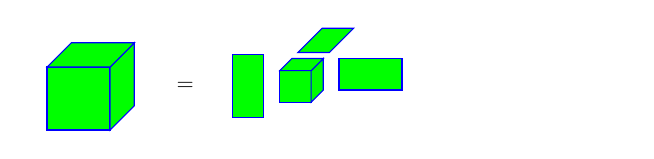
\begin{tikzpicture}[scale=0.2, every node/.style={transform shape}]
		\pgfmathsetmacro{\cubex}{4}
		\pgfmathsetmacro{\cubey}{4}
		\pgfmathsetmacro{\cubez}{4}
		\draw[blue,fill=pastelgreen] (-12,1,\cubez-2) -- ++(-\cubex,0,0) -- ++(0,-\cubey,0) -- ++(\cubex,0,0) -- cycle;
		\draw[blue,fill=pastelgreen] (-12,1,\cubez-2) -- ++(0,0,-\cubez) -- ++(0,-\cubey,0) -- ++(0,0,\cubez) -- cycle;
		\draw[blue,fill=pastelgreen] (-12,1,\cubez-2) -- ++(-\cubex,0,0) -- ++(0,0,-\cubez) -- ++(\cubex,0,0) -- cycle;
		\node[draw=none, text=black, scale=4] at (-8,-1,0) {$=$};
		
		\pgfmathsetmacro{\cubex}{2}
		\pgfmathsetmacro{\cubey}{2}
		\pgfmathsetmacro{\cubez}{2}
		\draw[blue,fill=pastelgreen] (0,0,0) -- ++(-\cubex,0,0) -- ++(0,-\cubey,0) -- ++(\cubex,0,0) -- cycle;
		\draw[blue,fill=pastelgreen] (0,0,0) -- ++(0,0,-\cubez) -- ++(0,-\cubey,0) -- ++(0,0,\cubez) -- cycle;
		\draw[blue,fill=pastelgreen] (0,0,0) -- ++(-\cubex,0,0) -- ++(0,0,-\cubez) -- ++(\cubex,0,0) -- cycle;
		
		\draw[blue,fill=pastelgreen] (-\cubex-1,1,0) -- ++(-\cubex,0,0) -- ++(0,-\cubey-2,0) -- ++(\cubex,0,0) -- cycle;
		\draw[blue,fill=pastelgreen] (\cubex+2+1,0,-\cubey) -- ++(-\cubex-2,0,0) -- ++(0,-\cubey,0) -- ++(\cubex+2,0,0) -- cycle;
		
		\draw[blue,fill=pastelgreen] (0,0,-\cubez-1) -- ++(-\cubex,0,0) -- ++(0,0,-\cubez-2) -- ++(\cubex,0,0) -- cycle;
		
		\path (-18,0) -- (20,0);
		\end{tikzpicture}
	\end{center}
	%%\vfill
	\item Tensor Train decomposition (equivalently known as Matrix Product States)
		
		\vspace*{-0.15cm}\begin{center}
		\begin{tikzpicture}[scale=0.2, every node/.style={transform shape}]
		
		\node (t0) at (0,-2.75) [scale=4] {\tensor{A}};
		\node [scale=4]at (2.5, -2.75) {$=$};
		\path (5,-6) -- (0,0);
		\end{tikzpicture}\hspace*{-0.15cm}
		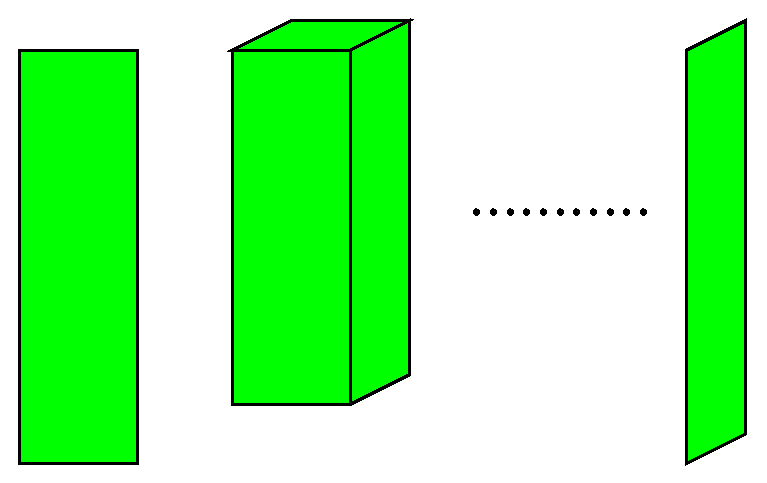
\includegraphics[scale=0.175]{./diagrams/ttentry-simple.eps}$\qquad\qquad$
	\end{center}
	\vspace*{-0.28cm}
	\noindent Tensor notation: bold letters denote tensors, i.e., {\scriptsize \tensor{A}} $\in \mathbb{R}^{n_1 \times \ldots \times n_d}$ is a $d$-dimensional tensor.
%%	\\
%%	\noindent \tensor{A} is represented with $2$ matrices and $d$-$2$ $3$-dimensional tensors. 
	%%\vfill
\end{itemize}
%%\end{block}
}
\end{frame}


%%%------------------------------------------------
%%\begin{frame}{Tensor Train decomposition}
%%%%\begin{itemize}
%%%%\item A $d$-dimensional tensor is represented with $2$ matrices and $d$-$2$ $3$-dimensional tensors.
%%%%\end{itemize}
%%
%%%%\begin{figure}
%%
%%\vspace*{-0.25cm}\begin{center}
%%\begin{tikzpicture}[scale=0.5, every node/.style={transform shape}]
%%
%%\node (t0) at (0,0) [scale=2.5] {\tensor{A}};
%%\node [scale=2]at (2, 0.0) {$=$};
%%\path (5,-6) -- (0,0);
%%\end{tikzpicture}
%%\includegraphics[scale=0.325]{./diagrams/ttentry.eps}
%%\end{center}
%%%%\end{figure}
%%\vspace*{-0.15cm}
%%\begin{itemize}
%%	\item Tensor notation: bold letters denote tensors, i.e., \tensor{A} $\in \mathbb{R}^{n_1 \times \ldots \times n_d}$ is a $d$-dimensional tensor 
%%	\item \tensor{A} is represented with $2$ matrices and $d$-$2$ $3$-dimensional tensors.
%%%%	\item An entry is computed by multiplying corresponding matrix (or row/column) of each core.
%%%%	\item For $n_1=\cdots=n_d=n$ and $r_1=\cdots=r_{d-1}=r$, the number of entries = $\mathcal{O}(ndr^2)$
%%\end{itemize}
%%\end{frame}

%%\begin{frame}{Tensor Train Representation}
%%
%%\begin{block}{}
%%$\tensor{A}$ $\in$ $\mathbb{R}^{n_1 \times \cdots \times n_d}$ is represented with cores $\tensor{G}_k$$\in$ $\mathbb{R}^{r_{k-1}\times n_k\times r_k}$, $k$=$1,2,\cdots d$, $r_0$=$r_d$=$1$ and its elements satisfy the following expression:
%%{\small\begin{align*}
%%\tensor{A}(i_1,\cdots ,i_d) 
%%&= \sum_{\alpha_0 = 1}^{r_0} \cdots \sum_{\alpha_d = 1}^{r_d} \tensor{G}_1(\alpha_0, i_1, \alpha_1) \cdots \tensor{G}_d(\alpha_{d-1}, i_d, \alpha_d)\\
%%&= \sum_{\alpha_1 = 1}^{r_1} \cdots \sum_{\alpha_{d-1} = 1}^{r_{d-1}} \tensor{G}_1(1, i_1, \alpha_1) \cdots \tensor{G}_d(\alpha_{d-1}, i_d, 1)
%%\end{align*}}
%%\begin{center}
%%\begin{tikzpicture}[scale=0.625, every node/.style={transform shape}]
%%\tikzstyle{taskc}=[circle, draw=orange, minimum size=11mm, fill=none, dashed, ultra thick]
%%\tikzstyle{taskr}=[draw=black, minimum height=8mm, minimum width=15mm, anchor=south west, fill=pastelgreen, text=black]
%%
%%\node(t1) at (0,0) {};
%%\node [above right=0cm and 0cm of t1.mid,taskr](T1) {$\textcolor{blue}{i_1}\alpha_1$};
%%\node [above right=0cm and 0.8cm of T1.south east, taskc](C1) {$\alpha_1$};
%%\node [above right=0cm and 0.8cm of C1.south east, taskr](T2) {$\alpha_1\textcolor{blue}{i_2}\alpha_2$};
%%\node [above right=0cm and 0.8cm of T2.south east, taskc](C2) {$\alpha_2$};
%%
%%\node [above right=0cm and 4.5cm of T2.south east, taskc](Cd) {$\alpha_{d\text{-}1}$};
%%\node [above right=0cm and 0.8cm of Cd.south east, taskr](Td) {$\alpha_{d\text{-}1}\textcolor{blue}{i_d}$};
%%\draw (T1.east)--(C1.west);
%%\draw (C1.east)--(T2.west);
%%\draw (T2.east)--(C2.west);
%%\draw [dotted] (C2.east)--(Cd.west);
%%\draw (Cd.east)--(Td.west);
%%\path (-0.1, -0.4) -- (2.5, -0.4); 
%%%%\path (-0.1, -0.8) -- (2.5, -0.8); 
%%\end{tikzpicture}
%%\end{center}
%%\end{block}
%%\begin{itemize}
%%\item For $n_1=n_2=\cdots=n_d=n$ and $r_1=r_2=\cdots=r_{d-1}=r$, the number of entries = $\mathcal{O}(ndr^2)$
%%\end{itemize}
%%\end{frame}


\begin{frame}
\frametitle{Previous Activities}
%%\tableofcontents[currentsection]
\tableofcontents


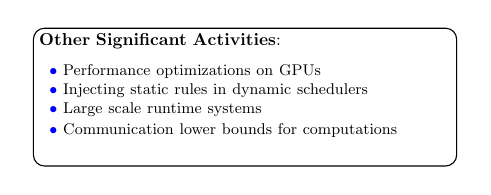
\begin{tikzpicture}[scale=0.625, every node/.style={transform shape}]
\tikzstyle{taskr}=[draw=black, rounded corners, minimum height=28mm, minimum width=86mm, fill=none, text=black]

\path (0,0) --(1,0);


\node (otheractivities) at (4,0) [taskr, anchor=south] {};
%%\node at (mainfocus.south) [below] {\textbf{Main focus}};

%%\node [below, align=left, text width=70mm]at (mainfocus.north) {		\textbf{$\ $Scalable communication optimal\\ $\ $algorithms for tensors\medskip}\\{\footnotesize \mybullet Analyze existing algorithms\\ 
%%		\mybullet Determine communication lower bounds\\\mybullet Propose communication optimal algorithms\\\mybullet Implement the proposed algorithms}};
%%
%%
%%\node (shorttermfocus) at (8,0) [taskr, minimum height=21mm, anchor=south] {};
%%\node at (shorttermfocus.south) [below] {\textbf{Short/Mid term plans}};
%%
%%\node [below, align=left, text width=70mm]at (shorttermfocus.north) {\textbf{$\ $Extension of existing approaches\medskip}\\\footnotesize \mybullet Strassen's concepts to tensors\\\mybullet Concepts of hierarchical matrices to tensors\\\mybullet Separation order of dimensions in tensor train};
%%
%%
%%\node (midtermfocus) at (16,0) [taskr, minimum height=25mm, anchor=south] {};
%%\node at (midtermfocus.south) [below] {\textbf{Mid/Long term plans}};
%%
%%\node [below, align=left, text width=70mm]at (midtermfocus.north) {\textbf{$\ $Exploratory topics\medskip}\\\footnotesize \mybullet New tensor representations\\ \mybullet Architecture aware algorithms\\ \mybullet Randomization in tensors\\ \mybullet Factorizations of tensors};

\node [below, align=left, text width=86mm]at (otheractivities.north) {
\textbf{$\ $Other Significant Activities}:\medskip\\{\small
\mybullet Performance optimizations on GPUs\\
\mybullet Injecting static rules in dynamic schedulers\\
\mybullet Large scale runtime systems\\
%%\mybullet Parallel tensor algorithms to perform molecular simulations\\
\mybullet Communication lower bounds for computations}};

\end{tikzpicture}
\end{frame}

%%\section{Performance Optimizations on GPUs for a Specific Application (\textcolor{green}{Not today})}


\section{Parallel Tensor Train Algorithms}

%%\subsection{Scheduling of Dense Linear Algebra Kernels}
%%\subsection{Communication Computation Overlap}


%%\subsection{Tensor Train Decomposition}
%%\begin{frame}{Tensor Train Decomposition}
%%content...
%%\end{frame}
%%\begin{frame}{Parallel Tensor Train Decomposition and Approximation Algorithms}
%%content...
%%\end{frame}
%%\begin{frame}{Unfolding Matrices of a Tensor \& Notations}
%%%%\begin{itemize}
%%%%	\item ($r_1, r_2,\cdots, r_{d-1}$) denotes the ranks of unfolding matrices of the tensor.
%%%%\end{itemize}
%%\end{frame}

\begin{frame}{Tensor Train algorithms and Separation of dimensions}

{\small\vspace*{-0.25cm}
\begin{itemize}
	\item A sequential algorithm to compute Tensor Train decomposition exists [Oseledets, 2011]  
\end{itemize}
\begin{minipage}{0.425\linewidth}
\begin{block}{Sequential algorithm}
	\begin{center}
		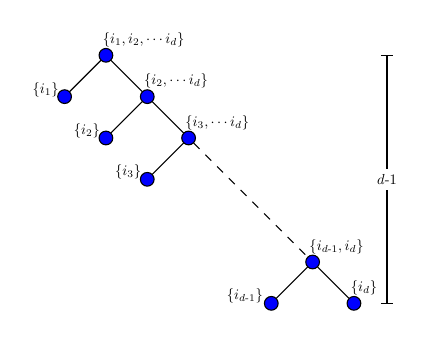
\begin{tikzpicture}[scale=0.525, every node/.style={transform shape}]
%%\draw[fill=cyan] (0,0) circle (0.8cm);
%%		\node [draw,circle]{r};
%%		\tikzstyle{task}=[circle, draw, minimum size=10mm]
%%		\node (d) at (0,0)[task, fill=babyblueeyes] {$D$};
%%		\node (e) at (2.5,0)[task, fill=pastelviolet] {$E$};
%%		\draw[thick, ->] (d.east) -- (e);
%%		
%%		\node (a) at (0,2)[task, fill=pastelyellow] {$A$};
%%		\node (b) at (2.5,2.75)[task, fill=pastelgreen] {$B$};
%%		\node (c) at (2.5,1.25)[task, fill=pastelred] {$C$};
%%		
%%		\draw[thick, ->] (a.east) -- (b);
%%		\draw[thick, ->] (a.east) -- (c);
\tikzstyle{taskc}=[circle, draw=black, minimum size=2mm, fill=blue]
\tikzstyle{taskr}=[draw=none, minimum height=2mm, minimum width=5mm, anchor=south west, fill=none, text=black]
%%
\node (t01) at (0,0) [taskc]{};
\node (t11) at (-1,-1) [taskc] {};
\node (t12) at (1, -1) [taskc] {};
\node (t21) at (0, -2) [taskc] {};
\node (t22) at (2, -2) [taskc] {};
\node (t31) at (1,-3) [taskc] {};
\node (t52) at (5, -5) [taskc] {};
\node (t61) at (4, -6) [taskc] {};
\node (t62) at (6, -6) [taskc] {};

\draw (t01) -- (t11);
\draw (t01) -- (t12);
\draw (t12) -- (t21);
\draw (t12) -- (t22);
\draw (t22) -- (t31);
\draw [dashed] (t22) -- (t52);
\draw (t52) -- (t61);
\draw (t52) -- (t62);

\draw (6.8, -6) -- (6.8, -3.25);
\draw (6.8, -2.75) -- (6.8, 0);

\draw (6.65, -6) -- (6.95, -6);
\draw (6.65, -0) -- (6.95, 0);
\node at (6.8, -3) {$d\text{-}1$};

\node [above left=0mm and 2mm of t01.mid, taskr](l01) {$\{i_1,i_2,\cdots i_d\}$};
\node [below left=2mm and 9mm of t11.mid, taskr](l11) {$\{i_1\}$};
\node [above left=0mm and 2mm of t12.mid, taskr](l12) {$\{i_2,\cdots i_d\}$};
\node [below left=2mm and 9mm of t21.mid, taskr](l21) {$\{i_2\}$};
\node [above left=0mm and 2mm of t22.mid, taskr](l22) {$\{i_3,\cdots i_d\}$};
\node [below left=2mm and 9mm of t31.mid, taskr](l31) {$\{i_3\}$};

\node [above left=0mm and 2mm of t52.mid, taskr](l52) {$\{i_{d\text{-}1}, i_d\}$};
\node [below left=2mm and 12mm of t61.mid, taskr](l61) {$\{i_{d\text{-}1}\}$};
\node [above left=0mm and 2mm of t62.mid, taskr](l62) {$\{i_d\}$};

\path (-0.1, -6.4) -- (2.5, -6.4); 
\end{tikzpicture}
\end{center}
\end{block}
\end{minipage}$\qquad$
\begin{minipage}{0.475\linewidth}
\begin{block}{For better parallelization}
\begin{center}
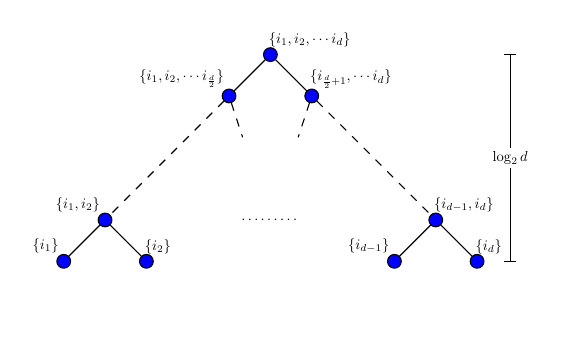
\begin{tikzpicture}[scale=0.525, every node/.style={transform shape}]

\tikzstyle{taskc}=[circle, draw=black, minimum size=2mm, fill=blue]
%%	\tikzstyle{taskr}=[draw=none, minimum height=2mm, minimum width=5mm, anchor=south west, fill=none, text=black]


\node (t01) at (0,0) [taskc]{};
\node (t11) at (-1,-1) [taskc] {};
\node (t12) at (1, -1) [taskc] {};

\node (tinter1) at (-0.5,-2) [taskc, draw=none, fill=none] {};
\node (tinter2) at (0.5,-2) [taskc, draw=none, fill=none] {};

\node (t41) at (-4,-4) [taskc] {};
\node (t42) at (4,-4) [taskc] {};
\node (t51) at (-5,-5) [taskc] {};
\node (t52) at (-3,-5) [taskc] {};
\node (t53) at (3,-5) [taskc] {};
\node (t54) at (5,-5) [taskc] {};


\draw (t01) -- (t11);
\draw (t01) -- (t12);

\draw [dashed] (t11) -- (tinter1.west);
\draw [dashed] (t12) -- (tinter2.east);

\draw [dashed] (t11) -- (t41);
\draw [dashed] (t12) -- (t42);

\path (t41) -- (t42) node [midway] {$\cdots\cdots\cdots$};

\draw (t41) -- (t51);
\draw (t41) -- (t52);

\draw (t42) -- (t53);
\draw (t42) -- (t54);


\draw (5.8, -5) -- (5.8, -2.75);
\draw (5.8, -2.25) -- (5.8, 0);

\draw (5.65, -5) -- (5.95, -5);
\draw (5.65, 0) -- (5.95, 0);
\node at (5.8, -2.5) {$\log_2 d$};

\node [above right] at (t01.160) {$\{i_1,i_2,\cdots i_d\}$};	

\node [above left] at (t11.mid) {$\{i_1,i_2,\cdots i_\frac{d}{2}\}$};	
\node [above right] at (t12.160) {$\{i_{\frac{d}{2}+1},\cdots i_d\}$};

\node [above left] at (t41.mid) {$\{i_1,i_2\}$};
\node [above right] at (t42.160) {$\{i_{d-1}, i_d\}$};

\node [above left] at (t51.mid) {$\{i_1\}$};
\node [above right] at (t52.160) {$\{i_2\}$};

\node [above left] at (t53.mid) {$\{i_{d-1}\}$};
\node [above right] at (t54.160) {$\{i_d\}$};


\path (-0.1, -6.4) -- (2.5, -6.4); 
%%		\path (-6.5, 0) -- (0,0);
\end{tikzpicture}
\end{center}
\end{block}
\end{minipage}
\begin{itemize}
	\item Can obtain better parallelism by expressing the operation in a balanced binary tree shape
	\begin{itemize}
		\item Proposed a parallel algorithm based on this idea ({\scriptsize joint work with L. Grigori, Inria Paris})
	\end{itemize}
\end{itemize}
}\end{frame}

%%\begin{frame}{Separatation of Dimensions \only<1>{in Sequential Algorithm }\only<2>{for Maximum Parallelization}}
%%\begin{block}{}
%%	\begin{center}
%%	\onslide<1->{
%%
%%	}
%%	\onslide<2->{
%%
%%	}
%%	\end{center}
%%\end{block}
%%\end{frame}

%%%%\begin{frame}{Unfolding matrices of a tensor}
%%%%
%%%%{\small
%%%%\vspace*{-0.15cm}\begin{block}{}
%%%%	\begin{center}
%%%%		\begin{tikzpicture}[scale=0.475, every node/.style={transform shape}]
%%%%%%\draw[fill=cyan] (0,0) circle (0.8cm);
%%%%%%		\node [draw,circle]{r};
%%%%%%		\tikzstyle{task}=[circle, draw, minimum size=10mm]
%%%%%%		\node (d) at (0,0)[task, fill=babyblueeyes] {$D$};
%%%%%%		\node (e) at (2.5,0)[task, fill=pastelviolet] {$E$};
%%%%%%		\draw[thick, ->] (d.east) -- (e);
%%%%%%		
%%%%%%		\node (a) at (0,2)[task, fill=pastelyellow] {$A$};
%%%%%%		\node (b) at (2.5,2.75)[task, fill=pastelgreen] {$B$};
%%%%%%		\node (c) at (2.5,1.25)[task, fill=pastelred] {$C$};
%%%%%%		
%%%%%%		\draw[thick, ->] (a.east) -- (b);
%%%%%%		\draw[thick, ->] (a.east) -- (c);
%%%%\tikzstyle{taskc}=[circle, draw=black, minimum size=2mm, fill=blue]
%%%%\tikzstyle{taskr}=[draw=none, minimum height=2mm, minimum width=5mm, anchor=south west, fill=none, text=black]
%%%%%%
%%%%\node (t01) at (0,0) [taskc]{};
%%%%\node (t11) at (-1,-1) [taskc] {};
%%%%\node (t12) at (1, -1) [taskc] {};
%%%%\node (t21) at (0, -2) [taskc] {};
%%%%\node (t22) at (2, -2) [taskc] {};
%%%%\node (t31) at (1,-3) [taskc] {};
%%%%\node (t52) at (5, -5) [taskc] {};
%%%%\node (t61) at (4, -6) [taskc] {};
%%%%\node (t62) at (6, -6) [taskc] {};
%%%%
%%%%\draw (t01) -- (t11);
%%%%\draw (t01) -- (t12);
%%%%\draw (t12) -- (t21);
%%%%\draw (t12) -- (t22);
%%%%\draw (t22) -- (t31);
%%%%\draw [dashed] (t22) -- (t52);
%%%%\draw (t52) -- (t61);
%%%%\draw (t52) -- (t62);
%%%%
%%%%\draw (6.8, -6) -- (6.8, -3.25);
%%%%\draw (6.8, -2.75) -- (6.8, 0);
%%%%
%%%%\draw (6.65, -6) -- (6.95, -6);
%%%%\draw (6.65, -0) -- (6.95, 0);
%%%%\node at (6.8, -3) {$d\text{-}1$};
%%%%
%%%%\node [above left=0mm and 2mm of t01.mid, taskr](l01) {$\{i_1,i_2,\cdots i_d\}$};
%%%%\node [below left=2mm and 9mm of t11.mid, taskr](l11) {$\{i_1\}$};
%%%%\node [above left=0mm and 2mm of t12.mid, taskr](l12) {$\{i_2,\cdots i_d\}$};
%%%%\node [below left=2mm and 9mm of t21.mid, taskr](l21) {$\{i_2\}$};
%%%%\node [above left=0mm and 2mm of t22.mid, taskr](l22) {$\{i_3,\cdots i_d\}$};
%%%%\node [below left=2mm and 9mm of t31.mid, taskr](l31) {$\{i_3\}$};
%%%%
%%%%\node [above left=0mm and 2mm of t52.mid, taskr](l52) {$\{i_{d\text{-}1}, i_d\}$};
%%%%\node [below left=2mm and 12mm of t61.mid, taskr](l61) {$\{i_{d\text{-}1}\}$};
%%%%\node [above left=0mm and 2mm of t62.mid, taskr](l62) {$\{i_d\}$};
%%%%
%%%%\path (-0.1, -6.4) -- (2.5, -6.4); 
%%%%\end{tikzpicture}$\qquad$
%%%%\begin{tikzpicture}[scale=0.475, every node/.style={transform shape}]
%%%%
%%%%\tikzstyle{taskc}=[circle, draw=black, minimum size=2mm, fill=blue]
%%%%%%	\tikzstyle{taskr}=[draw=none, minimum height=2mm, minimum width=5mm, anchor=south west, fill=none, text=black]
%%%%
%%%%
%%%%\node (t01) at (0,0) [taskc]{};
%%%%\node (t11) at (-1,-1) [taskc] {};
%%%%\node (t12) at (1, -1) [taskc] {};
%%%%
%%%%\node (tinter1) at (-0.5,-2) [taskc, draw=none, fill=none] {};
%%%%\node (tinter2) at (0.5,-2) [taskc, draw=none, fill=none] {};
%%%%
%%%%\node (t41) at (-4,-4) [taskc] {};
%%%%\node (t42) at (4,-4) [taskc] {};
%%%%\node (t51) at (-5,-5) [taskc] {};
%%%%\node (t52) at (-3,-5) [taskc] {};
%%%%\node (t53) at (3,-5) [taskc] {};
%%%%\node (t54) at (5,-5) [taskc] {};
%%%%
%%%%
%%%%\draw (t01) -- (t11);
%%%%\draw (t01) -- (t12);
%%%%
%%%%\draw [dashed] (t11) -- (tinter1.west);
%%%%\draw [dashed] (t12) -- (tinter2.east);
%%%%
%%%%\draw [dashed] (t11) -- (t41);
%%%%\draw [dashed] (t12) -- (t42);
%%%%
%%%%\path (t41) -- (t42) node [midway] {$\cdots\cdots\cdots$};
%%%%
%%%%\draw (t41) -- (t51);
%%%%\draw (t41) -- (t52);
%%%%
%%%%\draw (t42) -- (t53);
%%%%\draw (t42) -- (t54);
%%%%
%%%%
%%%%\draw (5.8, -5) -- (5.8, -2.75);
%%%%\draw (5.8, -2.25) -- (5.8, 0);
%%%%
%%%%\draw (5.65, -5) -- (5.95, -5);
%%%%\draw (5.65, 0) -- (5.95, 0);
%%%%\node at (5.8, -2.5) {$\log_2 d$};
%%%%
%%%%\node [above right] at (t01.160) {$\{i_1,i_2,\cdots i_d\}$};	
%%%%
%%%%\node [above left] at (t11.mid) {$\{i_1,i_2,\cdots i_\frac{d}{2}\}$};	
%%%%\node [above right] at (t12.160) {$\{i_{\frac{d}{2}+1},\cdots i_d\}$};
%%%%
%%%%\node [above left] at (t41.mid) {$\{i_1,i_2\}$};
%%%%\node [above right] at (t42.160) {$\{i_{d-1}, i_d\}$};
%%%%
%%%%\node [above left] at (t51.mid) {$\{i_1\}$};
%%%%\node [above right] at (t52.160) {$\{i_2\}$};
%%%%
%%%%\node [above left] at (t53.mid) {$\{i_{d-1}\}$};
%%%%\node [above right] at (t54.160) {$\{i_d\}$};
%%%%
%%%%
%%%%\path (-0.1, -6.4) -- (2.5, -6.4); 
%%%%%%		\path (-6.5, 0) -- (0,0);
%%%%\end{tikzpicture}
%%%%\end{center}
%%%%\end{block}
%%%%%%\begin{block}{$k$-th unfolding matrix}
%%%%	$k$-th unfolding matrix of tensor $\tensor{A}$ is defined as, $ A_k = [A_k(i_1, i_2,\cdots, i_k; i_{k+1},\cdots ,i_d)]$
%%%%	
%%%%	\begin{itemize}
%%%%		\item Size of $A_k$ is $(\prod_{l=1}^{k}n_l)\times(\prod_{l=k+1}^{d}n_l)$
%%%%		\item $r_k$ = rank($A_k$)
%%%%		\item Each node works with an unfolding matrix 
%%%%	\end{itemize}
%%%%%%\end{block}
%%%%\vspace*{-0.15cm}
%%%%\begin{block}{}
%%%%Theorem: Our parallel algorithm produces a Tensor Train representation with ranks not higher than $r_k$.
%%%%\end{block}
%%%%}\end{frame}

%%%%\begin{frame}{Diagramatic representation of our parallel algorithm}
%%%%\begin{columns}
%%%%	\begin{column}{0.425\linewidth}{\footnotesize
%%%%
%%%%}\end{column}
%%%%\begin{column}{0.575\linewidth}
%%%%\begin{center}
%%%%	\begin{tikzpicture}[scale=0.5, every node/.style={transform shape}]
%%%%	\tikzstyle{taskr}=[draw=black, minimum height=8mm, minimum width=8mm, fill=none, text=black]
%%%%	%%	anchor=south west,
%%%%	\node (t10) at (0,1.2) {$\tensor{A}(i_1,i_2,i_3,i_4,i_5,i_6)$};	
%%%%	\node (b01) at (0,0) [taskr]{};
%%%%	\node [above] at (b01.north) {$i_4i_5i_6$};
%%%%	\node [left] at (b01.west) {$i_1i_2i_3$};		
%%%%	
%%%%	\node (t11) at (-3,-1.8) {$\tensor{A}(i_1,i_2,i_3,\alpha_3)$};
%%%%	\node (t12) at (3,-1.8) {$\tensor{A}(\alpha_3, i_4, i_5, i_6)$};
%%%%	
%%%%	\draw (b01.south) -- (t11);	
%%%%	\draw (b01.south) -- (t12);
%%%%	
%%%%	\node (b11) at (-3,-3) [taskr]{};
%%%%	\node (b12) at (3,-3) [taskr]{};
%%%%	
%%%%	\node [above] at (b11.north) {$i_3\alpha_3$};
%%%%	\node [left] at (b11.west) {$i_1i_2$};
%%%%	
%%%%	\node [above] at (b12.north) {$i_6$};
%%%%	\node [left] at (b12.west) {$\alpha_3i_4i_5$};
%%%%	
%%%%	\node (t21) at (-5, -4.8) {$\tensor{A}(i_1,i_2,\alpha_2)$};
%%%%	\node (t22) at (-1.2, -4.8) {$\tensor{A}(\alpha_2, i_3,\alpha_3)$};
%%%%	
%%%%	\node (t23) at (1.2, -4.8) {$\tensor{A}(\alpha_3,i_4,i_5,\alpha_5)$};
%%%%	\node (t24) at (5, -4.8) {$\tensor{A}(\alpha_5, i_6)$};
%%%%	
%%%%	\draw (b11.south) -- (t21);
%%%%	\draw (b11.south) -- (t22);
%%%%	
%%%%	\draw (b12.south) -- (t23);
%%%%	\draw (b12.south) -- (t24);		
%%%%	
%%%%	\node (b21) at (-5,-6) [taskr]{};
%%%%	\node [above] at (b21.north) {$i_2\alpha_2$};
%%%%	\node [left] at (b21.west) {$i_1$};
%%%%	
%%%%	\node (b22) at (1.2,-6) [taskr]{};
%%%%	\node [above] at (b22.north) {$i_5\alpha_5$};
%%%%	\node [left] at (b22.west) {$\alpha_3i_4$};
%%%%	
%%%%	\node (t31) at (-6.25, -7.8) {$\tensor{A}(i_1,\alpha_1)$};
%%%%	\node (t32) at (-3.75, -7.8) {$\tensor{A}(\alpha_1,i_2,\alpha_2)$};
%%%%	
%%%%	\draw (b21.south) -- (t31);
%%%%	\draw (b21.south) -- (t32);
%%%%	
%%%%	\node (t33) at (0, -7.8) {$\tensor{A}(\alpha_3,i_4,\alpha_4)$};
%%%%	\node (t34) at (2.5, -7.8) {$\tensor{A}(\alpha_4,i_5,\alpha_5)$};
%%%%	
%%%%	\draw (b22.south) -- (t33);
%%%%	\draw (b22.south) -- (t34);
%%%%	
%%%%	\end{tikzpicture}
%%%%\end{center}
%%%%\end{column}
%%%%\end{columns}
%%%%
%%%%%%\begin{theorem}{\small
%%%%%%		Our parallel algorithm produces a Tensor Train representation with ranks not higher than $r_k$. It implies $\alpha_i \le r_i$ in the above diagram.}
%%%%%%\end{theorem}
%%%%\end{frame}


\begin{frame}{Tensor Train approximation algorithms}

{\footnotesize\vspace*{-0.15cm}
\begin{block}{Sequential algorithm [Oseledets, 2011]}
\begin{minipage}{0.35\linewidth}
	\begin{center}
		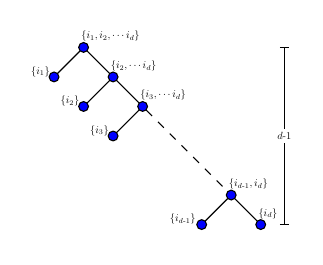
\begin{tikzpicture}[scale=0.375, every node/.style={transform shape}]
		%%\draw[fill=cyan] (0,0) circle (0.8cm);
		%%		\node [draw,circle]{r};
		%%		\tikzstyle{task}=[circle, draw, minimum size=10mm]
		%%		\node (d) at (0,0)[task, fill=babyblueeyes] {$D$};
		%%		\node (e) at (2.5,0)[task, fill=pastelviolet] {$E$};
		%%		\draw[thick, ->] (d.east) -- (e);
		%%		
		%%		\node (a) at (0,2)[task, fill=pastelyellow] {$A$};
		%%		\node (b) at (2.5,2.75)[task, fill=pastelgreen] {$B$};
		%%		\node (c) at (2.5,1.25)[task, fill=pastelred] {$C$};
		%%		
		%%		\draw[thick, ->] (a.east) -- (b);
		%%		\draw[thick, ->] (a.east) -- (c);
		\tikzstyle{taskc}=[circle, draw=black, minimum size=2mm, fill=blue]
		\tikzstyle{taskr}=[draw=none, minimum height=2mm, minimum width=5mm, anchor=south west, fill=none, text=black]
		%%
		\node (t01) at (0,0) [taskc]{};
		\node (t11) at (-1,-1) [taskc] {};
		\node (t12) at (1, -1) [taskc] {};
		\node (t21) at (0, -2) [taskc] {};
		\node (t22) at (2, -2) [taskc] {};
		\node (t31) at (1,-3) [taskc] {};
		\node (t52) at (5, -5) [taskc] {};
		\node (t61) at (4, -6) [taskc] {};
		\node (t62) at (6, -6) [taskc] {};
		
		\draw (t01) -- (t11);
		\draw (t01) -- (t12);
		\draw (t12) -- (t21);
		\draw (t12) -- (t22);
		\draw (t22) -- (t31);
		\draw [dashed] (t22) -- (t52);
		\draw (t52) -- (t61);
		\draw (t52) -- (t62);
		
		\draw (6.8, -6) -- (6.8, -3.25);
		\draw (6.8, -2.75) -- (6.8, 0);
		
		\draw (6.65, -6) -- (6.95, -6);
		\draw (6.65, -0) -- (6.95, 0);
		\node at (6.8, -3) {$d\text{-}1$};
		
		\node [above left=0mm and 2mm of t01.mid, taskr](l01) {$\{i_1,i_2,\cdots i_d\}$};
		\node [below left=2mm and 9mm of t11.mid, taskr](l11) {$\{i_1\}$};
		\node [above left=0mm and 2mm of t12.mid, taskr](l12) {$\{i_2,\cdots i_d\}$};
		\node [below left=2mm and 9mm of t21.mid, taskr](l21) {$\{i_2\}$};
		\node [above left=0mm and 2mm of t22.mid, taskr](l22) {$\{i_3,\cdots i_d\}$};
		\node [below left=2mm and 9mm of t31.mid, taskr](l31) {$\{i_3\}$};
		
		\node [above left=0mm and 2mm of t52.mid, taskr](l52) {$\{i_{d\text{-}1}, i_d\}$};
		\node [below left=2mm and 12mm of t61.mid, taskr](l61) {$\{i_{d\text{-}1}\}$};
		\node [above left=0mm and 2mm of t62.mid, taskr](l62) {$\{i_d\}$};
		
		\path (-0.1, -6.4) -- (2.5, -6.4); 
		\end{tikzpicture}
	\end{center}
\end{minipage}
\begin{minipage}{0.625\linewidth}

%%		\begin{block}{Approximation of a $d$ dimensional tensor}
%%			To obtain approximation error not more than $\epsilon$, at each node,
			\begin{itemize}
				\item Unfolding matrix: matricized representation of the tensor
				\item Perform truncated SVD of unfolding matrix $A$, $A=U\Sigma V^T + E_A$
%%				\item 
%%				\item Apply constant truncation $\frac{\epsilon}{\sqrt{d-1}}$, i.e., $||E_A||_F \le \frac{\epsilon}{\sqrt{d-1}}$
%%				\item Reshape $U$ as one of the tensor cores
				\item Work with $\Sigma V^T$ on the right subtree   
			\end{itemize}
%%		\end{block}

\end{minipage}	
\end{block}
\vspace*{-0.15cm}
\begin{block}{Our parallel algorithm}
\begin{minipage}{0.35\linewidth}
	\begin{center}
		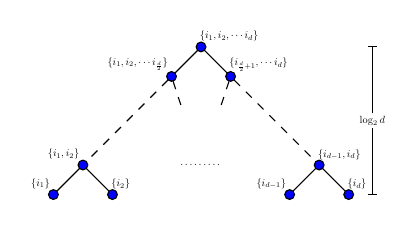
\begin{tikzpicture}[scale=0.375, every node/.style={transform shape}]
		
		\tikzstyle{taskc}=[circle, draw=black, minimum size=2mm, fill=blue]
		%%	\tikzstyle{taskr}=[draw=none, minimum height=2mm, minimum width=5mm, anchor=south west, fill=none, text=black]
		
		
		\node (t01) at (0,0) [taskc]{};
		\node (t11) at (-1,-1) [taskc] {};
		\node (t12) at (1, -1) [taskc] {};
		
		\node (tinter1) at (-0.5,-2) [taskc, draw=none, fill=none] {};
		\node (tinter2) at (0.5,-2) [taskc, draw=none, fill=none] {};
		
		\node (t41) at (-4,-4) [taskc] {};
		\node (t42) at (4,-4) [taskc] {};
		\node (t51) at (-5,-5) [taskc] {};
		\node (t52) at (-3,-5) [taskc] {};
		\node (t53) at (3,-5) [taskc] {};
		\node (t54) at (5,-5) [taskc] {};
		
		
		\draw (t01) -- (t11);
		\draw (t01) -- (t12);
		
		\draw [dashed] (t11) -- (tinter1.west);
		\draw [dashed] (t12) -- (tinter2.east);
		
		\draw [dashed] (t11) -- (t41);
		\draw [dashed] (t12) -- (t42);
		
		\path (t41) -- (t42) node [midway] {$\cdots\cdots\cdots$};
		
		\draw (t41) -- (t51);
		\draw (t41) -- (t52);
		
		\draw (t42) -- (t53);
		\draw (t42) -- (t54);
		
		
		\draw (5.8, -5) -- (5.8, -2.75);
		\draw (5.8, -2.25) -- (5.8, 0);
		
		\draw (5.65, -5) -- (5.95, -5);
		\draw (5.65, 0) -- (5.95, 0);
		\node at (5.8, -2.5) {$\log_2 d$};
		
		\node [above right] at (t01.160) {$\{i_1,i_2,\cdots i_d\}$};	
		
		\node [above left] at (t11.mid) {$\{i_1,i_2,\cdots i_\frac{d}{2}\}$};	
		\node [above right] at (t12.160) {$\{i_{\frac{d}{2}+1},\cdots i_d\}$};
		
		\node [above left] at (t41.mid) {$\{i_1,i_2\}$};
		\node [above right] at (t42.160) {$\{i_{d-1}, i_d\}$};
		
		\node [above left] at (t51.mid) {$\{i_1\}$};
		\node [above right] at (t52.160) {$\{i_2\}$};
		
		\node [above left] at (t53.mid) {$\{i_{d-1}\}$};
		\node [above right] at (t54.160) {$\{i_d\}$};
		
		
		%%\path (-0.1, -6.4) -- (2.5, -6.4); 
		%%		\path (-6.5, 0) -- (0,0);
		\end{tikzpicture}
	\end{center}
\end{minipage}
\begin{minipage}{0.625\linewidth}
%%		\begin{block}{Approximation of a $d$ dimensional tensor}
%%			To obtain approximation error less than  or close $\epsilon$, at each node,
			\begin{itemize}
				\item Perform truncated SVD of unfolding matrix $A$, $A=U\Sigma V^T + E_A$
				\item Find diagonal matrices $X$, $Y$, and $S$, such that $\Sigma=XSY$
%%				\item Apply truncation based on the number of dimensions
				\item Call left (resp. right) subtree with $UX$ (resp. $YV^T$)
%%				\item Call right subtree with $YV^T$
%%				\item Call right subtree with approximation error $\epsilon_1$
%%				\item If $U$ (resp. $V^T$) corresponds to more than one dimension, reshape  and call left (resp. right) subtree with approximation error $\epsilon_1$ (resp. $\epsilon_2$)
%%				%%		\item If $V^T$ corresponds to more than one dimension, reshape $YV^T$ and call right subtree with approximation error $\epsilon_2$
%%				\item $\epsilon_1$ and $\epsilon_2$ depend on $X$, $Y$, $S$ and $\epsilon$
			\end{itemize}
		$\qquad$Approach 1: $X=I$, $Y=\Sigma$, $S=I$
		
		$\qquad$Approach 2: $X=Y=\Sigma^{\frac{1}{2}}$, $S=I$
		
		$\qquad$Approach 3: $X=Y=\Sigma$, $S=\Sigma^{-1}$
%%		\begin{center}
%%	\begin{tabular}{cc}
%%		Approach 1: & $X=I$, $Y=\Sigma$, $S=I$\\
%%		Approach 2: & $X=Y=\Sigma^{\frac{1}{2}}$, $S=I$\\
%%		Approach 3: & $X=Y=\Sigma$, $S=\Sigma^{-1}$
%%	\end{tabular}
%%\end{center}
%%	\end{block}}
\end{minipage}
\end{block}
}\end{frame}

%%\begin{frame}{Aprroximations in Sequential Tensor Train Algorithms }
%%\vspace*{0.5cm}
%%
%%\begin{block}{}{\footnotesize
%%		\begin{itemize}
%%			\item Frobenius norm of a matrix $A$ is defined as, $||A||_F = \sqrt{\sum_{i,j} A(i;j)^2}$
%%			\item Frobenius norm of a $d$-dimensional tensor \tensor{A} is defined as, $||\tensor{A}||_F=$ $\sqrt{\sum_{i_1, i_2, \cdots, i_d}\tensor{A}(i_1,i_2,\cdots, i_d)^2 }$
%%	\end{itemize}}
%%\end{block}
%%
%%\end{frame}
%%\begin{frame}{Aprroximations in Parallel Tensor Train Algorithms}
%%
%%\bigskip
%%\begin{minipage}{0.5\linewidth}
%%{\footnotesize
%%		\begin{center}
%%			\begin{tabular}{cc}
%%				Approach 1: & $X=I$, $Y=\Sigma$, $S=I$\\
%%				Approach 2: & $X=Y=\Sigma^{\frac{1}{2}}$, $S=I$\\
%%				Approach 3: & $X=Y=\Sigma$, $S=\Sigma^{-1}$
%%			\end{tabular}
%%		\end{center}
%%}
%%\end{minipage}
%%%%\vfill
%%%%{\footnotesize
%%%%	\begin{block}{}
%%%%\begin{center}
%%%%
%%%%\end{center}\hfill
%%%%	\end{block}
%%%%}
%%%%{
%%%%\noindnet Approach 1: $X=I$, $Y=\Sigma$, $S=I$\\
%%%%\noindnet Approach 2: $X=Y=\Sigma^{\frac{1}{2}}$, $S=I$\\
%%%%\noindnet Approach 3: $X=Y=\Sigma$, $S=\Sigma^{-1}$
%%%%}
%%\end{frame}
%%\begin{frame}{Sequential Tensor Train Approximation}
%%\begin{itemize}
%%	\item Uniform truncation of $\Delta$=$\frac{\epsilon}{\sqrt{d-1}}$ is applied at each step
%%	\item $\Sigma_2$ is selected based on $\Delta$
%%	\item Approximation error of this approach is bounded by $\epsilon$
%%\end{itemize}
%%\end{frame}
%%
%%\begin{frame}{Parallel Tensor Train Approximation Algorithms}
%%\begin{itemize}
%%	\item We choose $X$, $S$, and $Y$ such that $XSY=\Sigma_1$
%%	\item We assume $\frac{\epsilon_1^2}{d_1^2} = \frac{\epsilon_2^2}{d_2^2}$
%%	\item $\Sigma_2$ is selected based on $\Delta$=$ \frac{\epsilon}{\sqrt{d-1}}$
%%	\item $\epsilon_1$ = f($\epsilon, \epsilon_2, \Delta, X, S, Y$) 
%%\end{itemize}
%% \includegraphics[scale=0.02]{./tmp/leadingSingularValuesPassed-1.jpg}
%% \includegraphics[scale=0.02]{./tmp/leadingSingularValuesPassed-2.jpg}
%%\end{frame}
%%
%%\begin{frame}{Accuracy of parallel approximation algorithms}
%%\begin{itemize}
%%	\item \textit{Leading Singular values to Right subtensor} (\hfirst)
%%	\item \textit{Square root of Leading Singular values to Both subtensors} (\hsecond)
%%	\item \textit{Leading Singular values to Both subtensors} (\hthird) 
%%\end{itemize}
%%	
%%\end{frame}

%%\begin{frame}{Low Rank Functions}
%%\begin{center}
%%	\begin{tabular}{|l|c|}
%%		\hline
%%		$Log$ & $\log(\sum_{j=1}^{N}j i_j)$\\ \hline
%%		$Sin$ & $\sin(\sum_{j=1}^{N}i_j)$\\ \hline
%%		Inverse-Square-Root ($ISR$) & $\frac{1}{\sqrt{\sum_{j=1}^{N}i_j^2}}$\\ \hline
%%		Inverse-Cube-Root ($ICR$) & $\frac{1}{\sqrt[3]{\sum_{j=1}^{N}i_j^3}}$\\ \hline
%%		Inverse-Penta-Root ($IPR$) & $\frac{1}{\sqrt[5]{\sum_{j=1}^{N}i_j^5}}$\\ \hline
%%	\end{tabular}
%%\end{center}
%%We consider $N=12$ and $i_j \in \{1, 2, 3, 4\}_{1\le j \le N}$. This setting produces a $12$-dimensional tensor with $4^{12}$ elements for each low rank function. Her we show results only for $Log$ tensor.
%%\end{frame}

\begin{frame}{Comparison of our approaches}

{\footnotesize\vspace*{-0.25cm}
\begin{itemize}
	\item A 12-dimensional tensor with $4^{12}$ elements (generated with a popular low rank function)
%%	, prescribed accuracy = $10^{-6}$
	\item prescribed accuracy = $10^{-6}$
	\item Compr: compression ratio, NE: number of elements, AA: approximation accuracy
\end{itemize}
	\begin{center}{\vspace*{-0.1cm}	
			\begin{tabular}{|c|c|c|c|c|}
				\hline
				& & \multicolumn{3}{|c|}{Parallel Algo}\\  \cline{3-5}
				Metric & Sequential Algo & Approach 1 & Approach 2 & Approach 3\\ \hline
				Compr & 99.993  & 99.817 & 99.799 & 99.993\\ \hline
				NE & 1212 & 30632 & 33772 & 1212\\ \hline
				AA & 2.271e-07 & 3.629e-08 & 2.820e-08 & 2.265e-07\\ \hline
			\end{tabular}
	}\end{center}
\vspace*{-0.25cm}
\begin{block}{SVD is expensive}
	\vspace*{-0.1cm}
\begin{itemize}
%%	\item SVD is expensive and hard to parallelize
	\item Good alternatives to SVD: QR factorization with column pivoting (QRCP), randomized SVD (RSVD)
\end{itemize}
\vspace*{-0.56cm}
	\begin{center}{
		\begin{tabular}{|c|c|c|c|c|c|}
			\hline
			Approach & Rank & Compr & NE & Sequential-AA & Approach3-AA\\ \hline
			{\scriptsize SVD} & \multirow{3}{*}{5} & \multirow{3}{*}{99.994} & \multirow{3}{*}{992} & 6.079e-06 & 6.079e-06\\ \cline{1-1} \cline{5-6}
			{\scriptsize QRCP+SVD} &  &  &  & 1.016e-05 & 1.384e-05\\ \cline{1-1} \cline{5-6}
			{\scriptsize RSVD} &  &  &  & 6.079e-06 & 6.079e-06\\ \hline
			
			
			{\scriptsize SVD} &\multirow{3}{*}{6} & \multirow{3}{*}{99.992} & \multirow{3}{*}{1376} & 1.323e-07 & 1.340e-07\\ \cline{1-1} \cline{5-6}
			{\scriptsize QRCP+SVD} & & & & 3.555e-07 & 5.737e-07\\ \cline{1-1} \cline{5-6}
			{\scriptsize RSVD} & & & & 1.322e-07& 1.322e-07\\ \hline
			
			
%%			SVD &\multirow{3}{*}{7} & \multirow{3}{*}{99.989} & \multirow{3}{*}{1824} & 2.753e-09 & 2.279e-08\\ \cline{1-1} \cline{5-6}
%%			QRCP+SVD & & & & 6.620e-09 & 1.167e-08\\ \cline{1-1} \cline{5-6}
%%			RSVD & & & & 2.760e-09 & 2.774e-09\\ \hline	
		\end{tabular}\vspace*{-0.05cm}
	}\end{center}
\end{block}
}
\end{frame}

%%\begin{frame}{Comparison of all Approaches}
%%We consider a $Log$ tensor generated with low rank function $\log(\sum_{j=1}^{d}j i_j)$. For $d=12$ and $i_j \in \{1, 2, 3, 4\}_{1\le j \le d}$, this function produces a $12$-dimensional tensor with $4^{12}$ elements.
%%
%%\begin{block}{Comparison of all approaches for Log tensor}
%%$\color{blue}{\bullet}$ Prescribed accuracy = $10^{-6}$\\
%%%%$\color{blue}{\bullet}$ Prototyped all approached in Matlab\\
%%$\color{blue}{\bullet}$ compr: compression ratio, ne: number of elements in aprroximation, OA: approximation accuracy
%%
%%\begin{center}{\small
%%	\begin{tabular}{|c|c|c|c|c|}
%%		\hline
%%		& & \multicolumn{3}{|c|}{Parallel Algo}\\  \cline{3-5}
%%		Metric & Sequential Algo & Approach 1 & Approach 2 & Approach 3\\ \hline
%%		compr & 99.993  & 99.817 & 99.799 & 99.993\\ \hline
%%		ne & 1212 & 30632 & 33772 & 1212\\ \hline
%%		OA & 2.271e-07 & 3.629e-08 & 2.820e-08 & 2.265e-07\\ \hline
%%	\end{tabular}
%%%		\begin{tabular}{|c|c|c|c|c|c|c|}
%%%			%%		\toprule
%%%			\hline
%%%			Appr. & Metric & $Log$ & $Sin$ & $ISR$ & $ICR$ & $IPR$\\ \hline
%%%			\multirow{3}{*} {\otta} & compr & 99.993 & 99.999 & 99.987 & 99.981 & 99.971 \\ \cline{2-7} 
%%%			& ne    & 1212 & 176 & 2240 & 3184 & 4864 \\ \cline{2-7} 
%%%			& OA    & 2.271e-07 & 2.615e-09 & 1.834e-07 & 4.884e-07 & 4.836e-07 \\ \cline{1-7} 
%%%			\multirow{3}{*} {\hfirst} & compr & 99.817 & 99.998 & 99.915 & 99.874 & 99.824 \\ \cline{2-7} 
%%%			& ne    & 30632 & 344 & 14196 & 21176 & 29524 \\ \cline{2-7} 
%%%			& OA    & 3.629e-08 & 1.412e-11 & 1.118e-07 & 8.520e-08 & 5.811e-08 \\ \cline{1-7} 
%%%			\multirow{3}{*} {\hsecond} & compr & 99.799 & 99.999 & 99.952 & 99.912 & 99.870 \\ \cline{2-7} 
%%%			& ne    & 33772 & 176 & 8068 & 14824 & 21792 \\ \cline{2-7} 
%%%			& OA    & 2.820e-08 & 6.144e-12 & 1.118e-07 & 8.518e-08 & 5.664e-08 \\ \cline{1-7} 
%%%			\multirow{3}{*} {\hthird} & compr & 99.993 & 99.999 & 99.987 & 99.981 & 99.970 \\ \cline{2-7} 
%%%			& ne    & 1212 & 176 & 2240 & 3184 & 4964 \\ \cline{2-7} 
%%%			& OA    & 2.265e-07 & 1.252e-11 & 1.834e-07 & 4.884e-07 & 3.999e-07 \\ \cline{1-7} 
%%%		\end{tabular}
%%}\end{center}
%%$\color{blue}{\bullet}$ Approach 3 performs the best among all parallel approaches -- will use only this for further comparison
%%%%$\color{blue}{\bullet}$  (leading singular values are passed on both sides of the tree)
%%\end{block}
%%\end{frame}
%%
%%
%%\begin{frame}{Alternatives to SVD}
%%\begin{itemize}
%%	\item SVD is expensive and hard to parallelize
%%	\item Good alternatives to SVD: QR factorization with column pivoting (QRCP), randomized SVD (RSVD)
%%\end{itemize}
%%\vspace*{-0.25cm}
%%\begin{block}{SVD vs QRCP+SVD vs RSVD for $Log$ tensor}
%%	\begin{center}
%%		\begin{tabular}{|c|c|c|c|c|c|}
%%			\hline
%%			Approach & Rank & compr & ne & Sequential-OA & Parallel-OA\\ \hline
%%			SVD & \multirow{3}{*}{5} & \multirow{3}{*}{99.994} & \multirow{3}{*}{992} & 6.079e-06 & 6.079e-06\\ \cline{1-1} \cline{5-6}
%%			QRCP+SVD &  &  &  & 1.016e-05 & 1.384e-05\\ \cline{1-1} \cline{5-6}
%%			RSVD &  &  &  & 6.079e-06 & 6.079e-06\\ \hline
%%			
%%			
%%			SVD &\multirow{3}{*}{6} & \multirow{3}{*}{99.992} & \multirow{3}{*}{1376} & 1.323e-07 & 1.340e-07\\ \cline{1-1} \cline{5-6}
%%			QRCP+SVD & & & & 3.555e-07 & 5.737e-07\\ \cline{1-1} \cline{5-6}
%%			RSVD & & & & 1.322e-07& 1.322e-07\\ \hline
%%			
%%			
%%			SVD &\multirow{3}{*}{7} & \multirow{3}{*}{99.989} & \multirow{3}{*}{1824} & 2.753e-09 & 2.279e-08\\ \cline{1-1} \cline{5-6}
%%			QRCP+SVD & & & & 6.620e-09 & 1.167e-08\\ \cline{1-1} \cline{5-6}
%%			RSVD & & & & 2.760e-09 & 2.774e-09\\ \hline	
%%		\end{tabular}
%%	\end{center}
%%\end{block}
%%\end{frame}

%%\begin{frame}{Comparison of All Approaches for the $Log$ tensor}
%%$\color{blue}{\bullet}$ Prescribed accuracy = $10^{-6}$\\
%%%%$\color{blue}{\bullet}$ Prototyped all approached in Matlab\\
%%$\color{blue}{\bullet}$ compr: compression ratio, ne: number of elements in aprroximation, OA: approximation accuracy
%%%%\begin{center}{\small
%%%%		\begin{tabular}{|c|c|c|c|c|c|c|}
%%%%			%%		\toprule
%%%%			\hline
%%%%			Appr. & Metric & $Log$ & $Sin$ & $ISR$ & $ICR$ & $IPR$\\ \hline
%%%%			\multirow{3}{*} {\otta} & compr & 99.993 & 99.999 & 99.987 & 99.981 & 99.971 \\ \cline{2-7} 
%%%%			& ne    & 1212 & 176 & 2240 & 3184 & 4864 \\ \cline{2-7} 
%%%%			& OA    & 2.271e-07 & 2.615e-09 & 1.834e-07 & 4.884e-07 & 4.836e-07 \\ \cline{1-7} 
%%%%			\multirow{3}{*} {\hfirst} & compr & 99.817 & 99.998 & 99.915 & 99.874 & 99.824 \\ \cline{2-7} 
%%%%			& ne    & 30632 & 344 & 14196 & 21176 & 29524 \\ \cline{2-7} 
%%%%			& OA    & 3.629e-08 & 1.412e-11 & 1.118e-07 & 8.520e-08 & 5.811e-08 \\ \cline{1-7} 
%%%%			\multirow{3}{*} {\hsecond} & compr & 99.799 & 99.999 & 99.952 & 99.912 & 99.870 \\ \cline{2-7} 
%%%%			& ne    & 33772 & 176 & 8068 & 14824 & 21792 \\ \cline{2-7} 
%%%%			& OA    & 2.820e-08 & 6.144e-12 & 1.118e-07 & 8.518e-08 & 5.664e-08 \\ \cline{1-7} 
%%%%			\multirow{3}{*} {\hthird} & compr & 99.993 & 99.999 & 99.987 & 99.981 & 99.970 \\ \cline{2-7} 
%%%%			& ne    & 1212 & 176 & 2240 & 3184 & 4964 \\ \cline{2-7} 
%%%%			& OA    & 2.265e-07 & 1.252e-11 & 1.834e-07 & 4.884e-07 & 3.999e-07 \\ \cline{1-7} 
%%%%		\end{tabular}
%%%%}\end{center}
%%
%%\begin{center}
%%	\begin{tabular}{|c|c|c|c|}
%%		\hline
%%		Approach & compr & ne & OA\\ \hline
%%		\otta & 99.993 & 1212 & 2.271e-07 \\ \hline
%%		\hfirst & 99.817 & 30632 & 3.629e-08 \\ \hline
%%		\hsecond & 99.799 & 33772 & 2.820e-08 \\ \hline
%%		\hthird & 99.993 & 1212 & 2.265e-07 \\ \hline
%%	\end{tabular}
%%\end{center}
%%\end{frame}

%%\begin{frame}{Accuracy Results}
%%\begin{itemize}
%%	\item SVD is expensive -- we also experimented with QRCP and Randomized SVD
%%\end{itemize}
%%\begin{center}
%%	\begin{tabular}{|c|c|c|c|c|}
%%		\hline
%%		Approach & Rank & compr & ne & OA\\ \hline
%%		SVD & 5 & 99.994 & 992 & 6.079e-06\\ \hline
%%		QRCP & 5 & 99.994 & 992 & 1.016e-05\\ \hline
%%		RSVD & 5 & 99.994 & 992 & 6.0791e-06\\ \hline
%%		
%%		SVD & 6 & 99.992 & 1376 & 1.323e-07\\ \hline
%%		QRCP & 6 & 99.992 & 1376 & 3.555e-07\\ \hline
%%		RSVD & 6 & 99.992 & 1376 & 1.3228e-07\\ \hline
%%		
%%		SVD & 7 & 99.989 & 1824 & 2.753e-09\\ \hline
%%		QRCP & 7 & 99.989 & 1824 & 6.620e-09\\ \hline
%%		RSVD & 7 & 99.989 & 1824 & 2.7602e-09\\ \hline
%%%%		
%%%%		\otta & 99.993 & 1212 & 2.271e-07 \\ \hline
%%%%		\hfirst & 99.817 & 30632 & 3.629e-08 \\ \hline
%%%%		\hsecond & 99.799 & 33772 & 2.820e-08 \\ \hline
%%%%		\hthird & 99.993 & 1212 & 2.265e-07 \\ \hline
%%	\end{tabular}
%%\end{center}
%%\end{frame}



\begin{frame}{Performance Comparison}
\begin{block}{Single core performance}
	\begin{columns}
		\begin{column}{0.4\textwidth}
			\begin{itemize}
				\item Number of computations for both RSVD algorithms = $\mathcal{O}(n^d)$
				\item Approach3-SVD is very slow
				\item Approach3-RSVD is much faster
%%				 than Sequential-SVD
%%				 (not in the diagram)
			\end{itemize}

		\end{column}
		\begin{column}{0.45\textwidth}
			\begin{center}
				\includegraphics[scale=0.35]{single-core-performance-seq-svd-rsvd-parallel-rsvd.eps}
%%				\includegraphics[scale=0.275]{single-core-performance-seq-svd-rsvd.eps}
%%				\includegraphics[scale=0.275]{single-core-performance-seq-parallel-rsvd.eps}
			\end{center}
		\end{column}
	\end{columns}
	
	
\end{block}
\begin{block}{Parallel performance counts along the critical path on $P$ processors}
	\begin{center}
		\begin{tabular}{|c|c|c|c|}
			\hline
			Algorithm & \# Computations& Communications & \# Messages\\ \hline
%%			Sequential-RSVD & $\mathcal{O}(\frac{n^d}{P})$ & $\mathcal{O}(\frac{n^{d-1}}{\sqrt{P}}\log{}P)$ & $\mathcal{O}(d\log{}P)$\\ \hline
			Sequential-RSVD & $\mathcal{O}(\frac{n^d}{P})$ & $\mathcal{O}(\frac{n^{d-1}}{P})$ & $\mathcal{O}(d\log{}P)$\\ \hline
			Approach3-RSVD & $\mathcal{O}(\frac{n^d}{P})$ & $\mathcal{O}(\frac{n^\frac{d}{2}}{\sqrt{P}}\log{}P)$ & $\mathcal{O}(\log{}d \log{}P)$\\ \hline
			%%		$\mathcal{O}(n\log{}n)$ 
		\end{tabular}
	\end{center}
\end{block}
\end{frame}

%%\begin{frame}{Performance Comparison}
%%\begin{itemize}
%%	\item Computation cost of the parallel algorithm decreases exponentially at each step
%%	\item Each algorithm runs on $P$ processors
%%\end{itemize}
%%Cost along the critical path:
%%\begin{center}
%%	\begin{tabular}{|c|c|c|c|}
%%		\hline
%%		Algorithm & Computation cost & Communication volume & Number of Messages\\ \hline
%%		Sequential & $\mathcal{O}(\frac{N^d}{P})$ & $\mathcal{O}(\frac{N^d}{\sqrt{P}}\log{}P)$ & $\mathcal{O}(d\log{}P)$\\ \hline
%%		Parallel & $\mathcal{O}(\frac{N^d}{P})$ & $\mathcal{O}(\frac{N^d}{\sqrt{P}}\log{}P)$ & $\mathcal{O}(\log{}d \log{}P)$\\ \hline
%%%%		$\mathcal{O}(n\log{}n)$ 
%%	\end{tabular}
%%\end{center}
%%
%%Cost along the critical path after the first step,
%%\begin{center}
%%	\begin{tabular}{|c|c|c|c|}
%%		\hline
%%		Algorithm & Computation cost & Communication volume & Number of Messages\\ \hline
%%		Sequential & $\mathcal{O}(\frac{N^{d-1}}{P})$ & $\mathcal{O}(\frac{N^{d-1}}{\sqrt{P}}\log{}P)$ & $\mathcal{O}(d\log{}P)$\\ \hline
%%		Parallel & $\mathcal{O}(\frac{N^\frac{d}{2}}{P})$ & $\mathcal{O}(\frac{N^\frac{d}{2}}{\sqrt{P}}\log{}P)$ & $\mathcal{O}(\log{}d \log{}P)$\\ \hline
%%		%%		$\mathcal{O}(n\log{}n)$ 
%%	\end{tabular}
%%\end{center}
%%\end{frame}



%%\subsection{Communication Optimal Algorithms for Tensors}





%%\section{Scheduling on Heterogeneous Systems}
%%\begin{frame}
%%\frametitle{Previous Research Activities}
%%\tableofcontents[currentsection]
%%\end{frame}



%%\begin{frame}{NWChemEX and TAMM}
%%content...
%%\end{frame}



%%\subsection{Scheduling of Dense Linear Algebra Kernels}
%%\begin{frame}
%%\frametitle{Table of Contents}
%%\tableofcontents[currentsubsection]
%%\end{frame}

\section{Scheduling on Heterogeneous Systems}

\begin{frame}{Scheduling on Heterogeneous Systems}

{\footnotesize
	\vspace*{-0.175cm}
	\begin{itemize}
				
		\item Heterogeneous systems are common in High Performance Computing (HPC) ({\scriptsize 147 out of 500 in TOP500 list})
		\vfill 
		\item Task based runtimes are a popular approach to exploit these systems
		
		\begin{columns}
		%%			\null \hfill
		\begin{column}{0.35\linewidth}
			%%			\begin{figure}
			\begin{center}
				\vspace*{-0.25cm}
				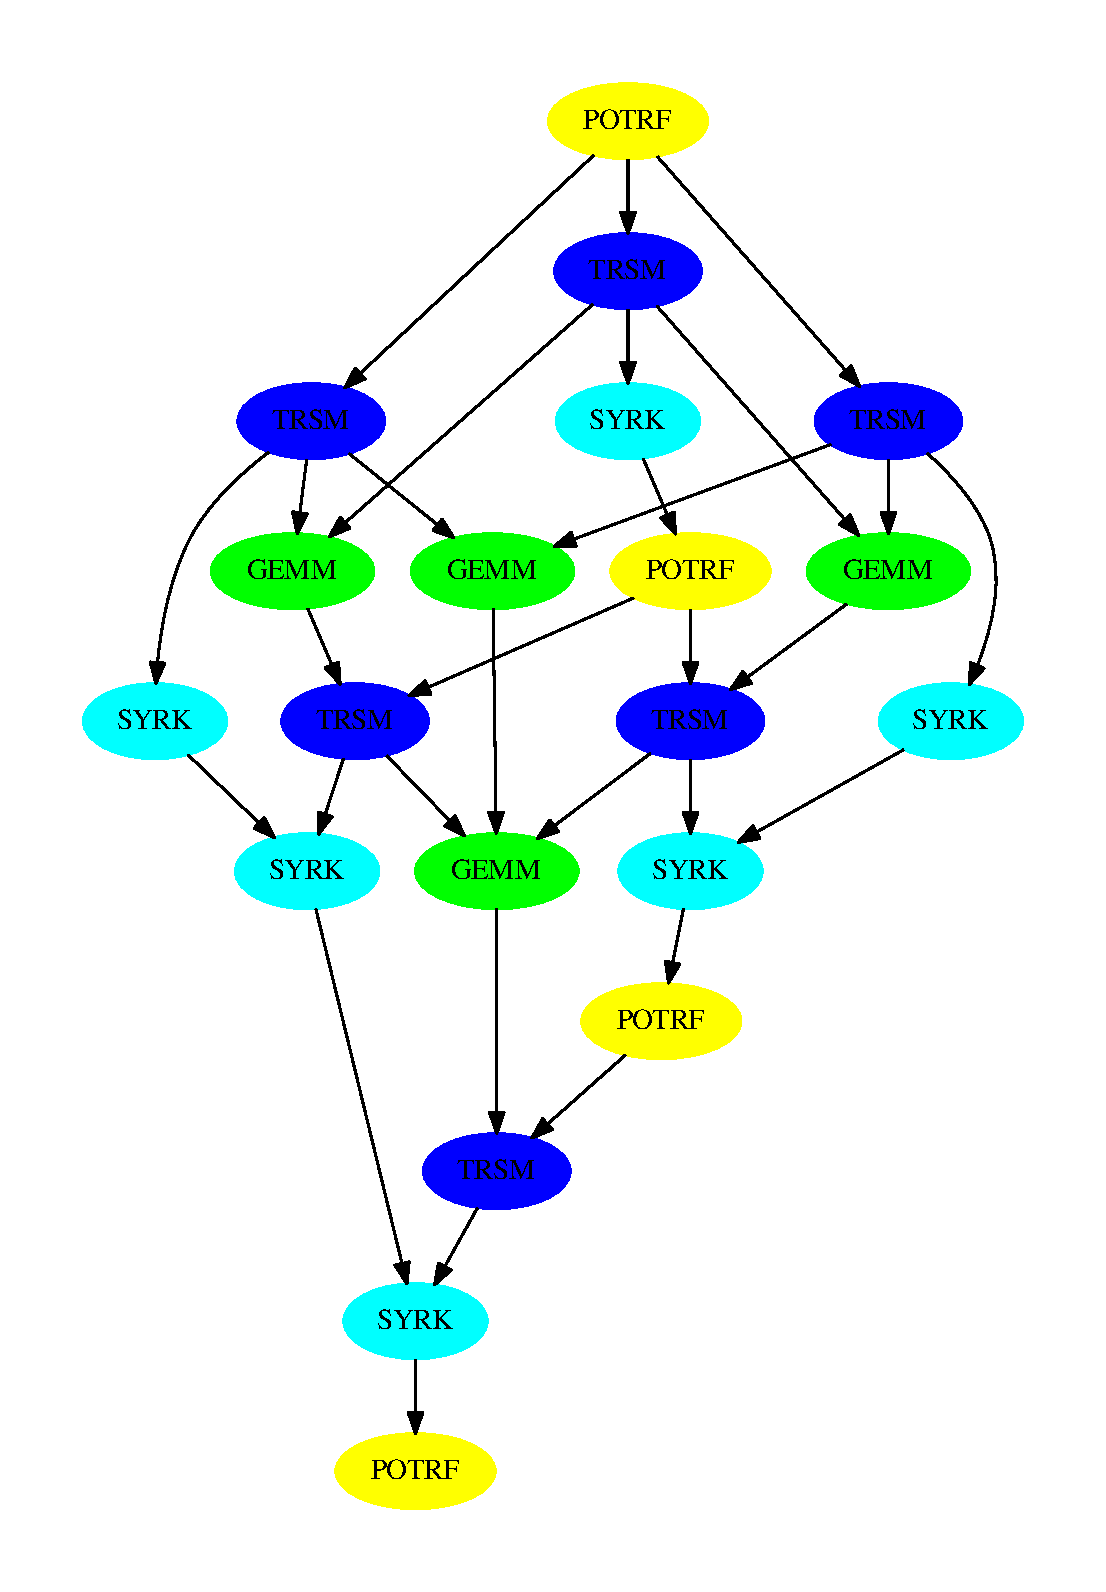
\includegraphics[scale=0.085]{./diagrams/choleskyWithoutId_4.pdf}
			\end{center}\vspace*{-0.35cm}
			%%			\caption{Cholesky task graph for $4\times4$ tile matrix}
			%%		\end{figure}
		\end{column}
		\begin{column}{0.745\linewidth}
			\begin{itemize}{\footnotesize
				\item Task based runtimes: StarPU, OmpSS, Legion, PaRSEC
				\item Application is represented as a graph of tasks (computations)
				\item E.g., Cholesky graph for $4\times4$ tile matrix
			}\end{itemize}
%%			\begin{itemize}
%%				\item Application is represented as a direct acyclic graph
%%				\item Vertices represent tasks (computations) and edges represent dependencies
%%				%%			\item Edges represent dependencies among tasks
%%				\vfill
%%				\item E.g., Cholesky graph for $4\times4$ tile matrix
%%			\end{itemize}
	\end{column}
		\end{columns}
	  

	\end{itemize}

	\vspace*{-0.225cm}
	
	\begin{block}{StarPU scheduler performance}
		\begin{minipage}{0.5\linewidth}
			\vspace*{-1.2cm}
			\begin{center}
				\includegraphics[scale=0.56]{./plots/Actual_vs_GEMMBound.eps}	
			\end{center}
			\vspace*{-1.25cm}
			%%\vspace*{-0.35cm}
			%%\begin{block}{}
		\end{minipage}$\quad$
		\begin{minipage}{0.45\linewidth}
			\begin{itemize}
				\item A platform with 9 CPUs and 3 GPUs
				\item Scheduler is based on popular heft strategy
			\end{itemize}
			\vspace*{-0.25cm}
			\begin{block}{}{
					%%		$\textcolor{green}{\bullet}$ Goal: Enhance performance bounds and propose better scheduling strategies \\
					%%		$\bullet$Goal: Propose approaches to enhance performance bounds and better scheduling strategies\\
					\setlength{\leftmargini}{1.5em}
					\begin{itemize}
						%%		\item A heterogeneous platform with 9 CPUs and 3 GPUs
						%%		\item StarPU scheduler is based on popular heft strategy
						\item Goal: Enhance performance bounds and propose better scheduling strategies
					\end{itemize}\vspace*{-0.15cm}
					%%			\mybullet Goal: Enhance performance bounds and propose better scheduling strategies\\
					%%			
					%%			
					\noindent {\tiny Joint work with E. Agullo, O. Beaumont, L. Eyraud-Dubois, and S. Thibault during my PhD at Inria Bordeaux}
					%%		$\bullet$Goal: Propose approaches to enhance performance bounds and better scheduling strategies
					%%	\begin{itemize}
					%%		\item Propose approaches to enhance performance bounds
					%%		\item Propose better scheduling strategies
					%%	\end{itemize}
			}\end{block}
		\end{minipage}
	\end{block}
	
	%%\begin{minipage}{0.475\linewidth}
	%%	\begin{block}{}{\scriptsize
	%%		%%		$\textcolor{green}{\bullet}$ Goal: Enhance performance bounds and propose better scheduling strategies \\
	%%		%%		$\bullet$Goal: Propose approaches to enhance performance bounds and better scheduling strategies\\
	%%		\setlength{\leftmargini}{1.5em}
	%%		\begin{itemize}
	%%			%%		\item A heterogeneous platform with 9 CPUs and 3 GPUs
	%%			%%		\item StarPU scheduler is based on popular heft strategy
	%%			\item Goal: Enhance performance bounds and propose better scheduling strategies
	%%		\end{itemize}\vspace*{-0.15cm}
	%%		\noindent {\tiny Joint work with E. Agullo, O. Beaumont, L. Eyraud-Dubois, and S. Thibault during my PhD at Inria Bordeaux}
	%%		%%		$\bullet$Goal: Propose approaches to enhance performance bounds and better scheduling strategies
	%%		%%	\begin{itemize}
	%%		%%		\item Propose approaches to enhance performance bounds
	%%		%%		\item Propose better scheduling strategies
	%%		%%	\end{itemize}
	%%}\end{block}
	%%\end{minipage}
	
}
\end{frame}





%%%%%%%\begin{frame}{Heterogeneous Systems \& Task Based Runtime Systems}
%%%%%\begin{frame}{Scheduling on Heterogeneous Systems}
%%%%%
%%%%%{\footnotesize
%%%%%	\vspace*{-0.175cm}
%%%%%	\begin{itemize}
%%%%%	%%	\item Challenges:
%%%%%	%%	\begin{itemize}
%%%%%	%%%%		\item Scheduling and resource allocation problems are NP hard
%%%%%%%	\item Performance share of accelerators increased from 28\% to 43\% in the last 5 years [Top500 list] 
%%%%%	\item  Significant performance share (more than 43\%) is produced by heterogeneous systems [Top500 list] 
%%%%%%%	\item Heterogeneous systems are common in High Performance Computing (HPC)
%%%%%	\vfill
%%%%%	\item Almost impossible to develop optimized hand tune kernels for all the systems
%%%%%%%	 architectures
%%%%%	%%		\item Hard to obtain precise estimation of duration of tasks and data transfers
%%%%%	%%	\end{itemize}
%%%%%	\vfill
%%%%%	\item Task based runtime systems, e.g., StarPU, OmpSS, Legion, PaRSEC
%%%%%\end{itemize}
%%%%%\begin{columns}
%%%%%	%%			\null \hfill
%%%%%	\begin{column}{0.25\linewidth}
%%%%%		%%			\begin{figure}
%%%%%		\begin{center}
%%%%%			\vspace*{-0.5cm}
%%%%%			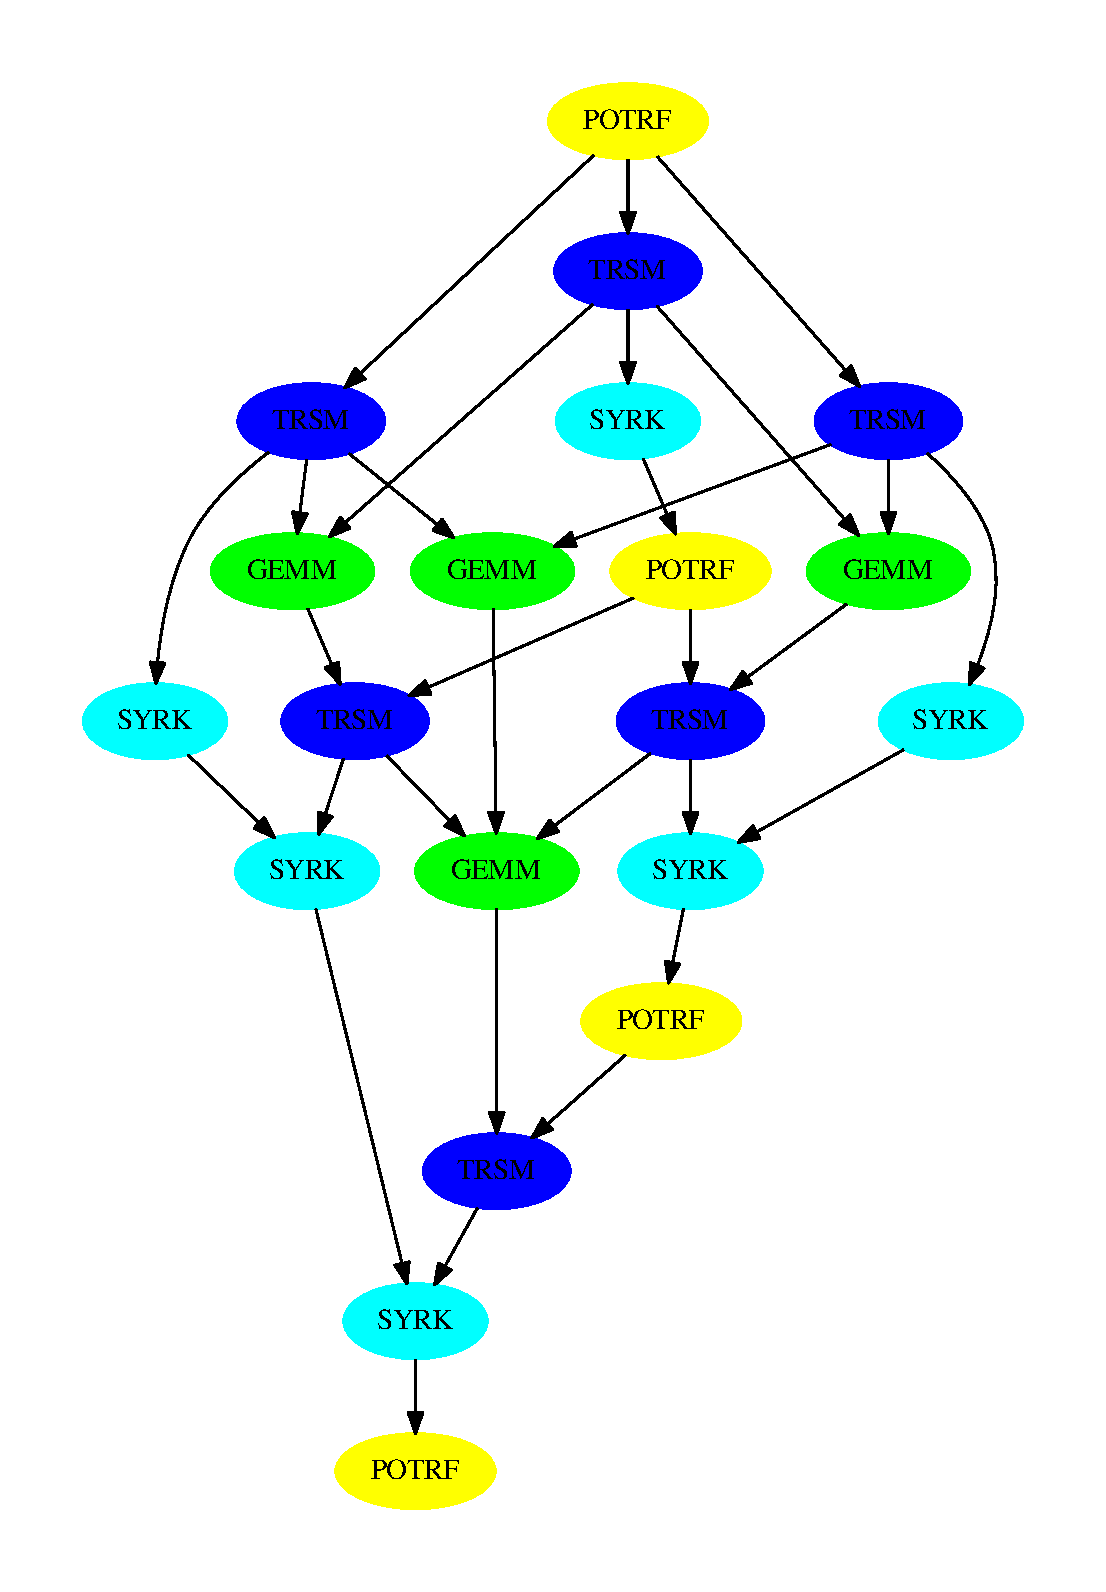
\includegraphics[scale=0.085]{./diagrams/choleskyWithoutId_4.pdf}
%%%%%		\end{center}\vspace*{-0.35cm}
%%%%%		%%			\caption{Cholesky task graph for $4\times4$ tile matrix}
%%%%%		%%		\end{figure}
%%%%%	\end{column}
%%%%%	\begin{column}{0.745\linewidth}
%%%%%		\begin{itemize}
%%%%%			\item Application is represented as a direct acyclic graph
%%%%%			\item Vertices represent tasks (computations) and edges represent dependencies
%%%%%%%			\item Edges represent dependencies among tasks
%%%%%			\vfill
%%%%%			\item E.g., Cholesky graph for $4\times4$ tile matrix
%%%%%		\end{itemize}
%%%%%	\end{column}
%%%%%\end{columns}
%%%%%	\vspace*{-0.225cm}
%%%%%
%%%%%	\begin{block}{StarPU scheduler performance}
%%%%%		\begin{minipage}{0.5\linewidth}
%%%%%		\vspace*{-1.2cm}
%%%%%		\begin{center}
%%%%%			\includegraphics[scale=0.56]{./plots/Actual_vs_GEMMBound.eps}	
%%%%%		\end{center}
%%%%%		\vspace*{-1.25cm}
%%%%%		%%\vspace*{-0.35cm}
%%%%%		%%\begin{block}{}
%%%%%	\end{minipage}$\quad$
%%%%%\begin{minipage}{0.45\linewidth}
%%%%%	\begin{itemize}
%%%%%		\item A platform with 9 CPUs and 3 GPUs
%%%%%		\item Scheduler is based on popular heft strategy
%%%%%	\end{itemize}
%%%%%\vspace*{-0.25cm}
%%%%%	\begin{block}{}{
%%%%%			%%		$\textcolor{green}{\bullet}$ Goal: Enhance performance bounds and propose better scheduling strategies \\
%%%%%			%%		$\bullet$Goal: Propose approaches to enhance performance bounds and better scheduling strategies\\
%%%%%			\setlength{\leftmargini}{1.5em}
%%%%%			\begin{itemize}
%%%%%				%%		\item A heterogeneous platform with 9 CPUs and 3 GPUs
%%%%%				%%		\item StarPU scheduler is based on popular heft strategy
%%%%%				\item Goal: Enhance performance bounds and propose better scheduling strategies
%%%%%			\end{itemize}\vspace*{-0.15cm}
%%%%%%%			\mybullet Goal: Enhance performance bounds and propose better scheduling strategies\\
%%%%%%%			
%%%%%%%			
%%%%%			\noindent {\tiny Joint work with E. Agullo, O. Beaumont, L. Eyraud-Dubois, and S. Thibault during my PhD at Inria Bordeaux}
%%%%%			%%		$\bullet$Goal: Propose approaches to enhance performance bounds and better scheduling strategies
%%%%%			%%	\begin{itemize}
%%%%%			%%		\item Propose approaches to enhance performance bounds
%%%%%			%%		\item Propose better scheduling strategies
%%%%%			%%	\end{itemize}
%%%%%	}\end{block}
%%%%%\end{minipage}
%%%%%	\end{block}
%%%%%
%%%%%%%\begin{minipage}{0.475\linewidth}
%%%%%%%	\begin{block}{}{\scriptsize
%%%%%%%		%%		$\textcolor{green}{\bullet}$ Goal: Enhance performance bounds and propose better scheduling strategies \\
%%%%%%%		%%		$\bullet$Goal: Propose approaches to enhance performance bounds and better scheduling strategies\\
%%%%%%%		\setlength{\leftmargini}{1.5em}
%%%%%%%		\begin{itemize}
%%%%%%%			%%		\item A heterogeneous platform with 9 CPUs and 3 GPUs
%%%%%%%			%%		\item StarPU scheduler is based on popular heft strategy
%%%%%%%			\item Goal: Enhance performance bounds and propose better scheduling strategies
%%%%%%%		\end{itemize}\vspace*{-0.15cm}
%%%%%%%		\noindent {\tiny Joint work with E. Agullo, O. Beaumont, L. Eyraud-Dubois, and S. Thibault during my PhD at Inria Bordeaux}
%%%%%%%		%%		$\bullet$Goal: Propose approaches to enhance performance bounds and better scheduling strategies
%%%%%%%		%%	\begin{itemize}
%%%%%%%		%%		\item Propose approaches to enhance performance bounds
%%%%%%%		%%		\item Propose better scheduling strategies
%%%%%%%		%%	\end{itemize}
%%%%%%%}\end{block}
%%%%%%%\end{minipage}
%%%%%
%%%%%}
%%%%%\end{frame}

%%%%\begin{frame}{Heterogeneous Systems \& Task Based Runtime Systems}
%%%%
%%%%{\footnotesize
%%%%\begin{minipage}{0.54\linewidth}
%%%%\begin{block}{Share of Accelerators: TOP500 list}
%%%%	\begin{center}
%%%%		\begin{tabular}{|c|c|c|}
%%%%			\hline
%%%%			Year & \#Systems & \% Performance share\\ \hline
%%%%			2015 & 103 & 28\\ \hline
%%%%			2020 & 147 & 43\\ \hline
%%%%		\end{tabular}
%%%%	\end{center}
%%%%\end{block}
%%%%{\scriptsize
%%%%\begin{block}{Task Based Runtime Systems}
%%%%	\begin{itemize}
%%%%		%%	\item Challenges:
%%%%		%%	\begin{itemize}
%%%%		%%%%		\item Scheduling and resource allocation problems are NP hard
%%%%		\item Almost impossible to develop optimized hand tune kernels for all architectures
%%%%%%		\item Hard to obtain precise estimation of duration of tasks and data transfers
%%%%		%%	\end{itemize}
%%%%		\vfill
%%%%		\item Task based runtime systems, e.g., StarPU, Legion, PaRSEC
%%%%	\end{itemize}
%%%%	\begin{columns}
%%%%		%%			\null \hfill
%%%%		\begin{column}{0.25\linewidth}
%%%%%%			\begin{figure}
%%%%			\begin{center}
%%%%				\vspace*{-0.45cm}
%%%%				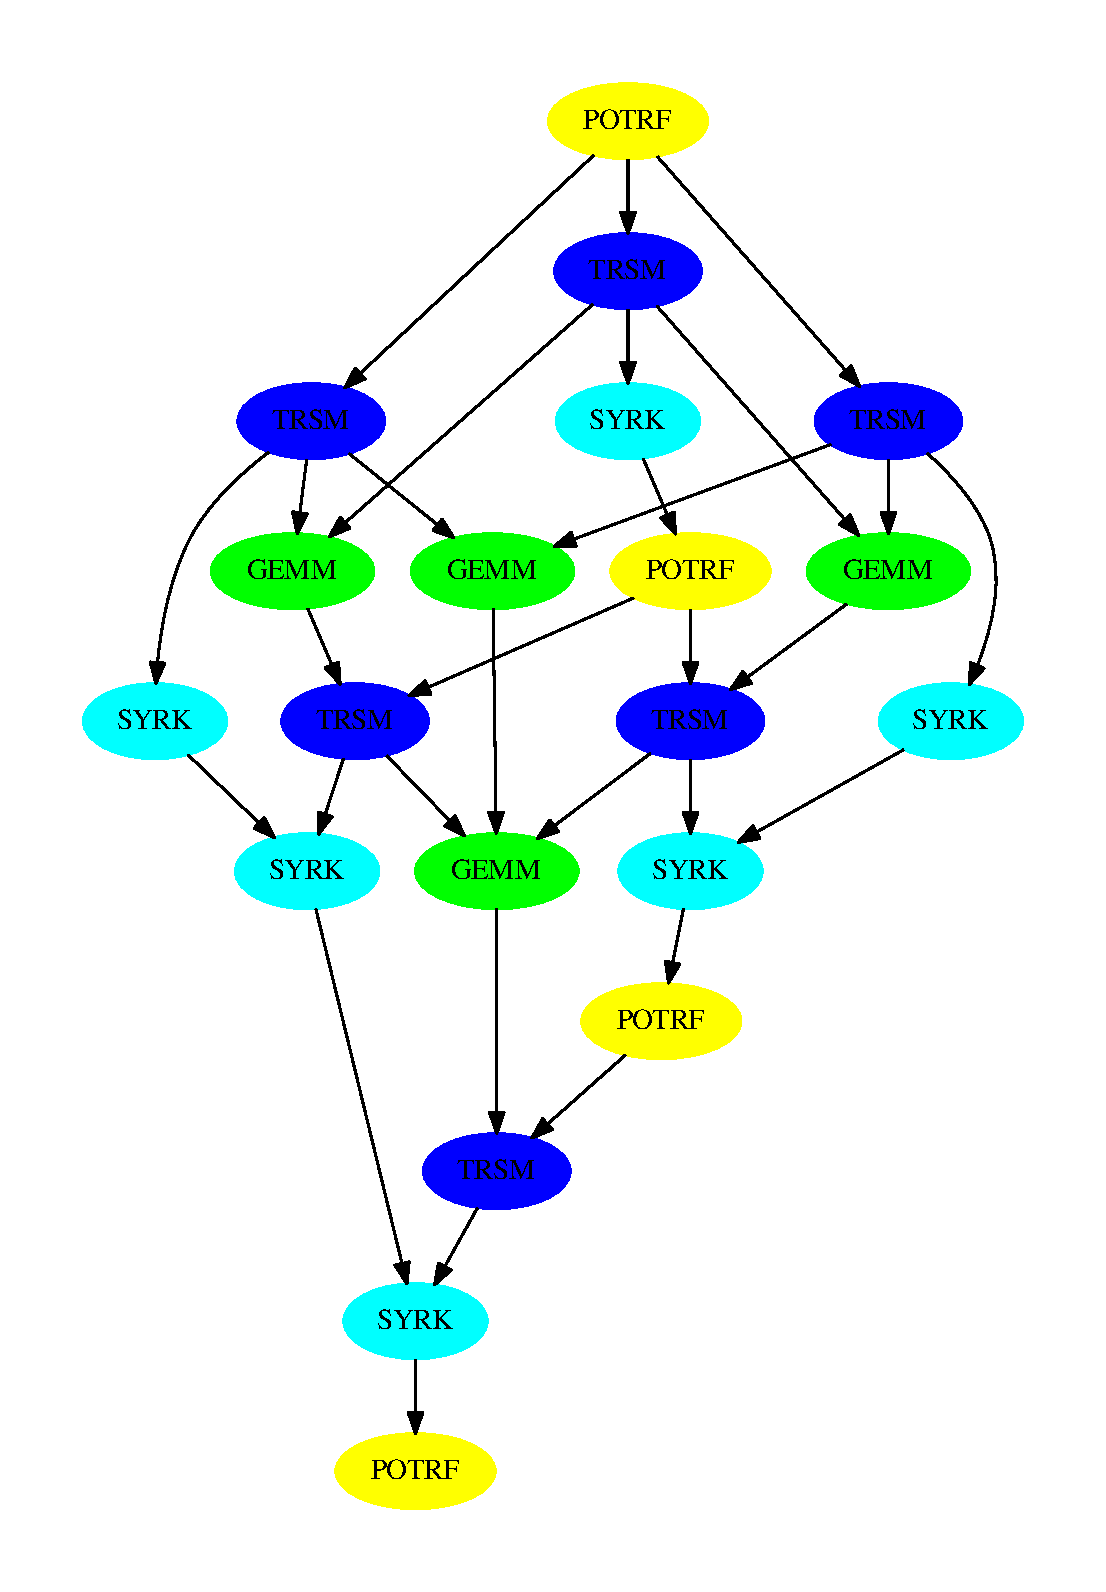
\includegraphics[scale=0.1]{./diagrams/choleskyWithoutId_4.pdf}
%%%%			\end{center}\vspace*{-0.35cm}
%%%%%%			\caption{Cholesky task graph for $4\times4$ tile matrix}
%%%%%%		\end{figure}
%%%%		\end{column}
%%%%		\begin{column}{0.745\linewidth}
%%%%			\begin{itemize}
%%%%				\item Application is represented as a direct acyclic graph (DAG)
%%%%				\item Vertices represent tasks (computations)
%%%%				\item Edges represent dependencies among tasks
%%%%				\vfill
%%%%				\item E.g., Cholesky DAG for $4\times4$ tile matrix
%%%%			\end{itemize}
%%%%		\end{column}
%%%%	\end{columns}
%%%%\end{block}}
%%%%\end{minipage}\hfill
%%%%\begin{minipage}{0.435\linewidth}
%%%%\begin{block}{StarPU scheduler performance}
%%%%	\begin{center}
%%%%		\includegraphics[scale=0.375]{./plots/Actual_vs_GEMMBound.eps}	
%%%%	\end{center}
%%%%\vspace*{-0.45cm}
%%%%%%\vspace*{-0.35cm}
%%%%%%\begin{block}{}
%%%%	{\scriptsize
%%%%		\begin{itemize}
%%%%			\item A platform with 9 CPUs and 3 GPUs
%%%%			\item Scheduler is based on popular heft strategy
%%%%			%%			\item Goal: propose approaches to enhance performance bounds and better scheduling strategies
%%%%		\end{itemize}
%%%%		%%		$\bullet$Goal: Propose approaches to enhance performance bounds and better scheduling strategies
%%%%		%%	\begin{itemize}
%%%%		%%		\item Propose approaches to enhance performance bounds
%%%%		%%		\item Propose better scheduling strategies
%%%%		%%	\end{itemize}
%%%%}
%%%%\end{block}
%%%%%%\end{block}
%%%%
%%%%\vspace*{-0.25cm}	
%%%%\begin{block}{}{\scriptsize
%%%%%%		$\textcolor{green}{\bullet}$ Goal: Enhance performance bounds and propose better scheduling strategies \\
%%%%%%		$\bullet$Goal: Propose approaches to enhance performance bounds and better scheduling strategies\\
%%%%    \setlength{\leftmargini}{1.5em}
%%%%		\begin{itemize}
%%%%			%%		\item A heterogeneous platform with 9 CPUs and 3 GPUs
%%%%			%%		\item StarPU scheduler is based on popular heft strategy
%%%%			\item Goal: Enhance performance bounds and propose better scheduling strategies
%%%%		\end{itemize}\vspace*{-0.15cm}
%%%%		\noindent {\tiny Joint work with E. Agullo, O. Beaumont, L. Eyraud-Dubois, and S. Thibault during my PhD at Inria Bordeaux}
%%%%		%%		$\bullet$Goal: Propose approaches to enhance performance bounds and better scheduling strategies
%%%%		%%	\begin{itemize}
%%%%		%%		\item Propose approaches to enhance performance bounds
%%%%		%%		\item Propose better scheduling strategies
%%%%		%%	\end{itemize}
%%%%}\end{block}
%%%%\end{minipage}
%%%%
%%%%
%%%%%%\begin{block}{Task Based Runtime Systems}
%%%%%%\begin{itemize}
%%%%%%	%%	\item Challenges:
%%%%%%	%%	\begin{itemize}
%%%%%%	%%%%		\item Scheduling and resource allocation problems are NP hard
%%%%%%	\item Almost impossible to develop optimized hand tune kernels for all architectures
%%%%%%	\item Hard to obtain precise estimation of duration of tasks and data transfers
%%%%%%	%%	\end{itemize}
%%%%%%	\vfill
%%%%%%	\item Task based runtime systems, Eg: StarPU, OmpSS, Legion, QUARK, PaRSEC
%%%%%%\end{itemize}
%%%%%%		\begin{columns}
%%%%%%%%			\null \hfill
%%%%%%			\begin{column}{0.35\linewidth}
%%%%%%				\begin{center}
%%%%%%					\vspace*{-0.25cm}
%%%%%%					\includegraphics[scale=0.175]{./diagrams/taskGraph.eps}
%%%%%%				\end{center}
%%%%%%			\end{column}
%%%%%%			\begin{column}{0.6\linewidth}
%%%%%%				\begin{itemize}
%%%%%%					\item Application is represented as a direct acyclic graph
%%%%%%					\item Vertices represent tasks (computations)
%%%%%%					\item Edges represent dependencies among tasks
%%%%%%					\vfill
%%%%%%				\end{itemize}
%%%%%%			\end{column}
%%%%%%		\end{columns}
%%%%%%\end{block}
%%%%}
%%%%\end{frame}

%%\begin{frame}{Tiled Cholesky Factorization}	
%%%%	\vfill
%%\begin{columns}
%%\begin{column}{0.56\linewidth}{\footnotesize
%%Input: a positive definite matrix, A with N $\times$ N tiles \\
%%Output: a lower triangular matrix L, A = LL$^\intercal$
%%\vspace*{-0.25cm}
%%\begin{algorithm}[H]
%%	\begin{algorithmic}[1]
%%		\FOR {$k = 0$ to $N-1$}
%%		\STATE L[k][k] $\leftarrow$ \textcolor{yellow}{POTRF}(A[k][k])\;
%%		\FOR {$i = k+1$ to $N-1$}
%%		\STATE L[i][k] $\leftarrow$ \textcolor{blue}{TRSM}(L[k][k], A[i][k])\;
%%		\ENDFOR
%%		\FOR {$j = k+1$ to $N-1$}
%%		\STATE A[j][j] $\leftarrow$ \textcolor{cyannew}{SYRK}(L[j][k], A[j][j])\;
%%		\FOR {$i = j+1$ to $N-1$}
%%		\STATE A[i][j] $\leftarrow$ \textcolor{greenhtml}{GEMM}(L[i][k], L[j][k], A[i][j])\;
%%		\ENDFOR
%%		\ENDFOR
%%		\ENDFOR			
%%	\end{algorithmic}
%%	\caption{Tiled Cholesky factorization}
%%\end{algorithm}
%%}\end{column}
%%	\begin{column}{0.4\linewidth}{\footnotesize
%%		\vspace*{-0.25cm}
%%		\begin{exampleblock}{Tiled Cholesky Task Graph (N=5)}
%%			\vspace*{-0.25cm}
%%			\begin{center}
%%				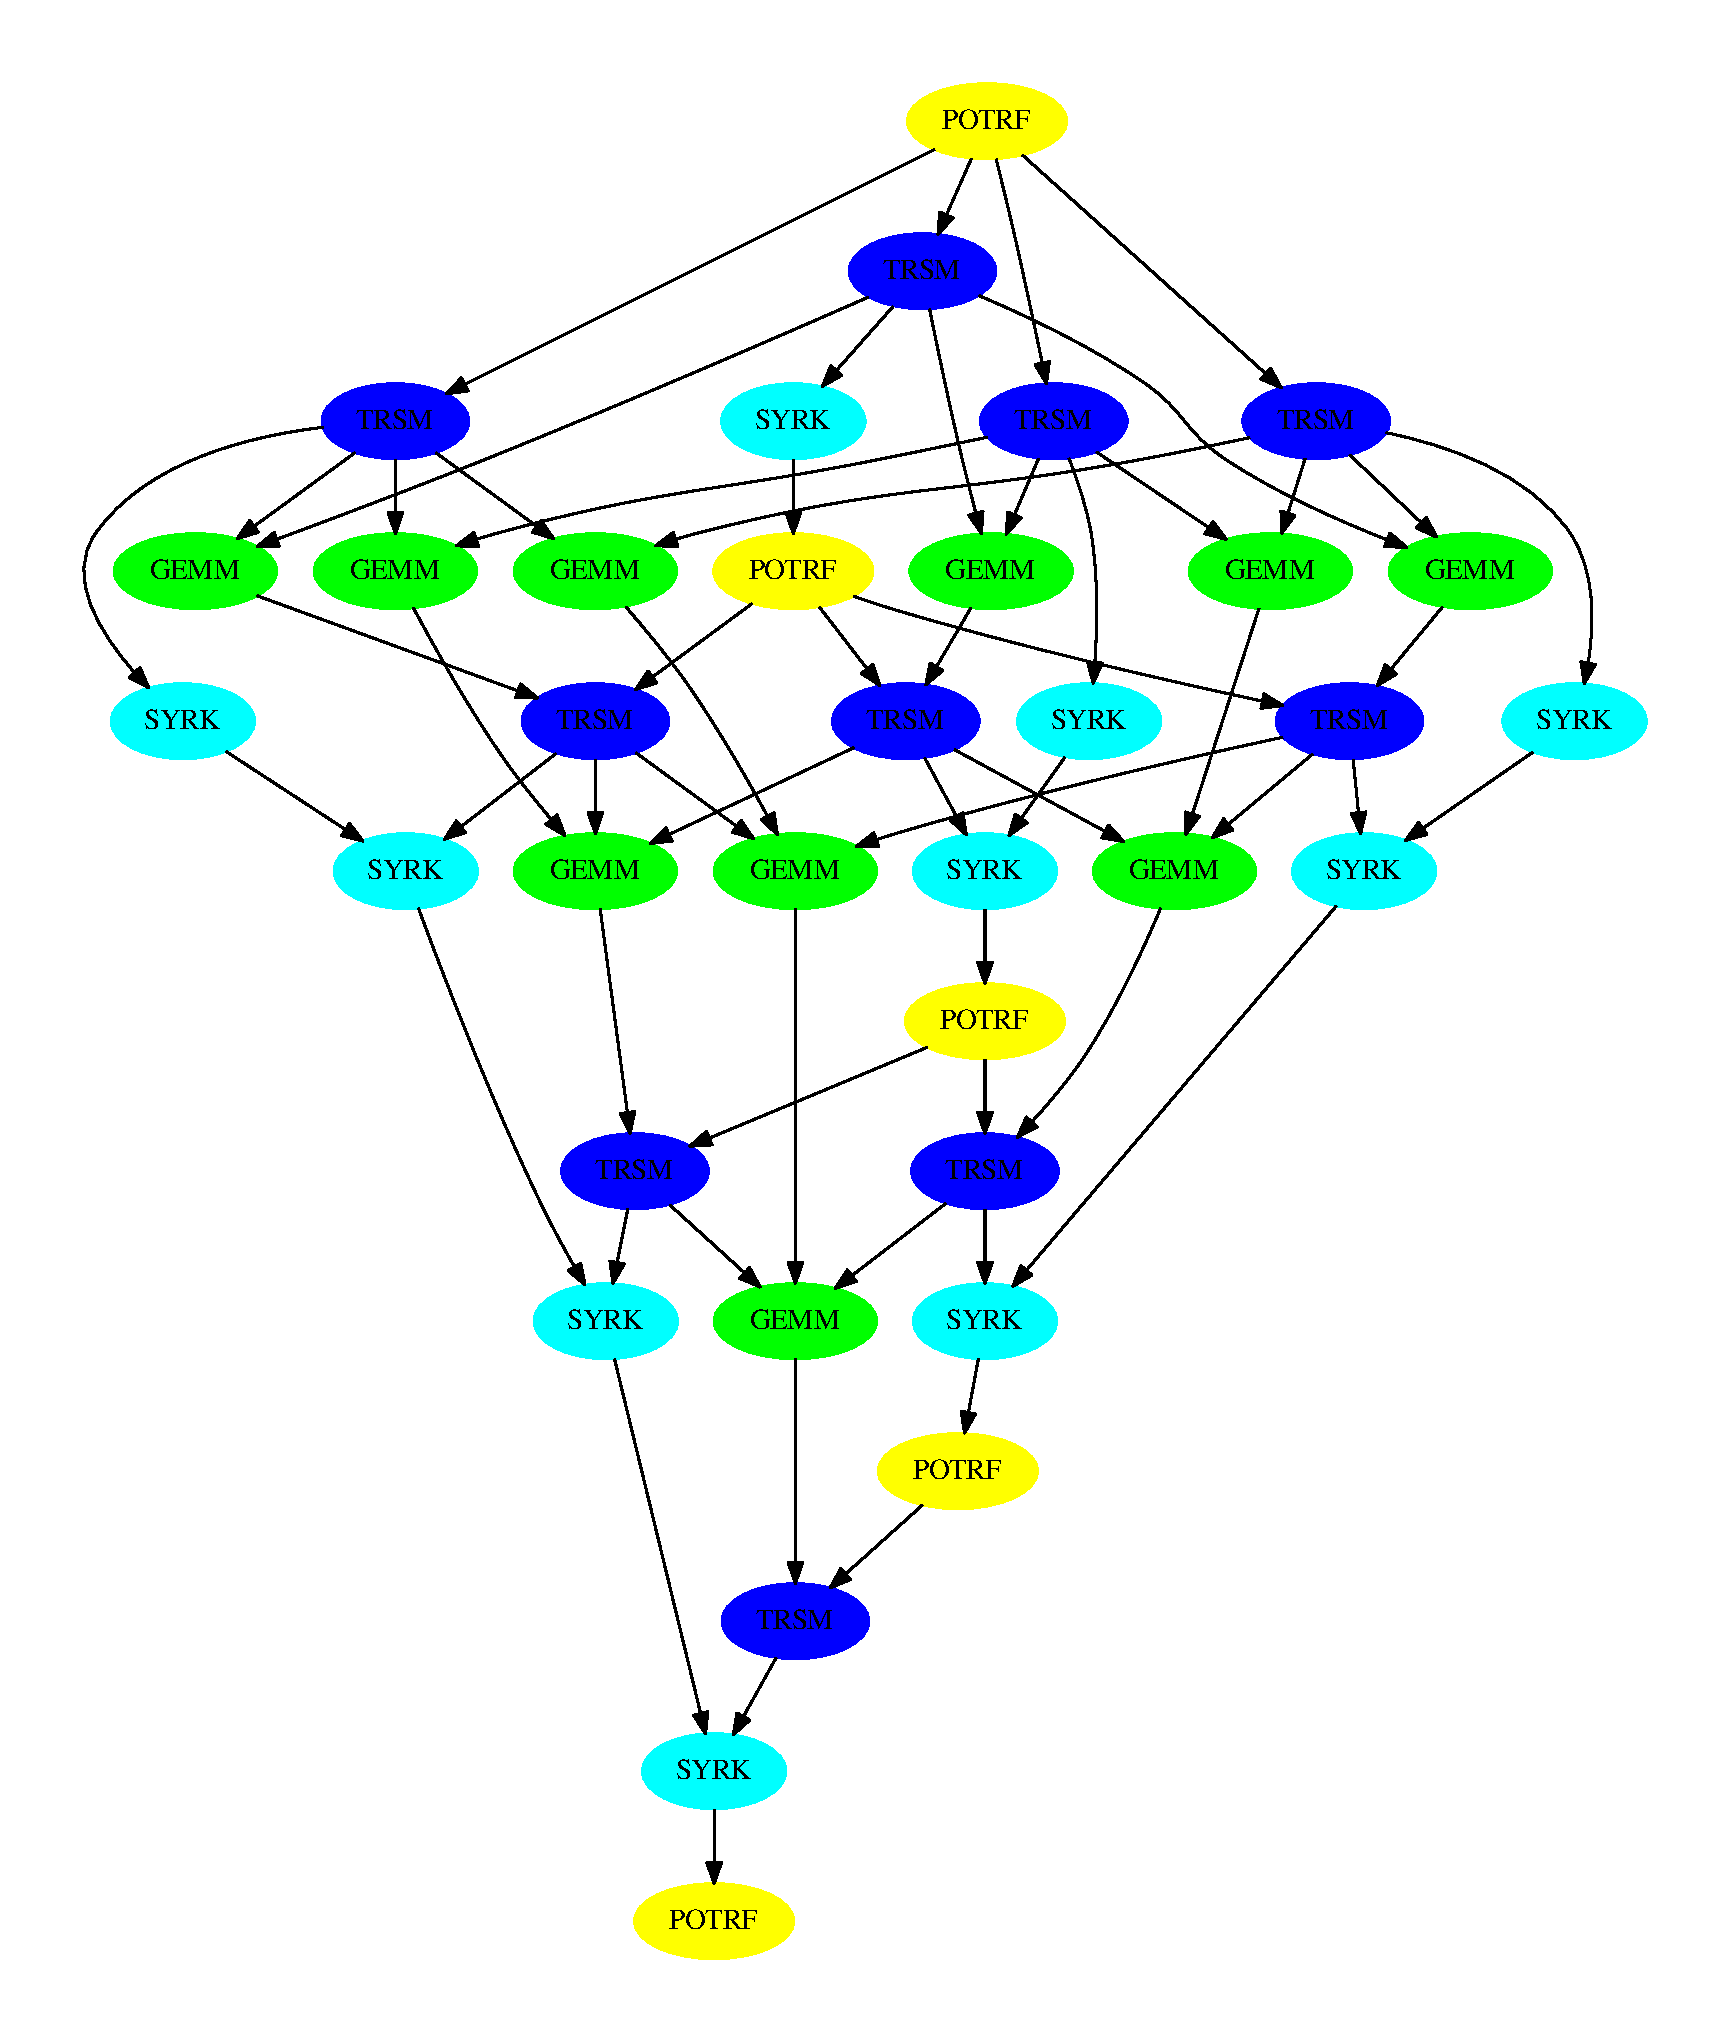
\includegraphics[scale=0.19]{./diagrams/choleskyWithoutId_5.pdf}
%%			\end{center}
%%		\end{exampleblock}
%%	}\end{column}
%%\end{columns} 
%%
%%\end{frame}


%%%%\begin{frame}{Performance vs Bounds of Cholesky Factorization}
%%%%\vspace*{-0.25cm}\begin{minipage}{0.4\linewidth}{\footnotesize
%%%%\begin{exampleblock}{Tiled Cholesky Task Graph (N=5)}\vspace*{-0.15cm}
%%%%	\begin{center}
%%%%		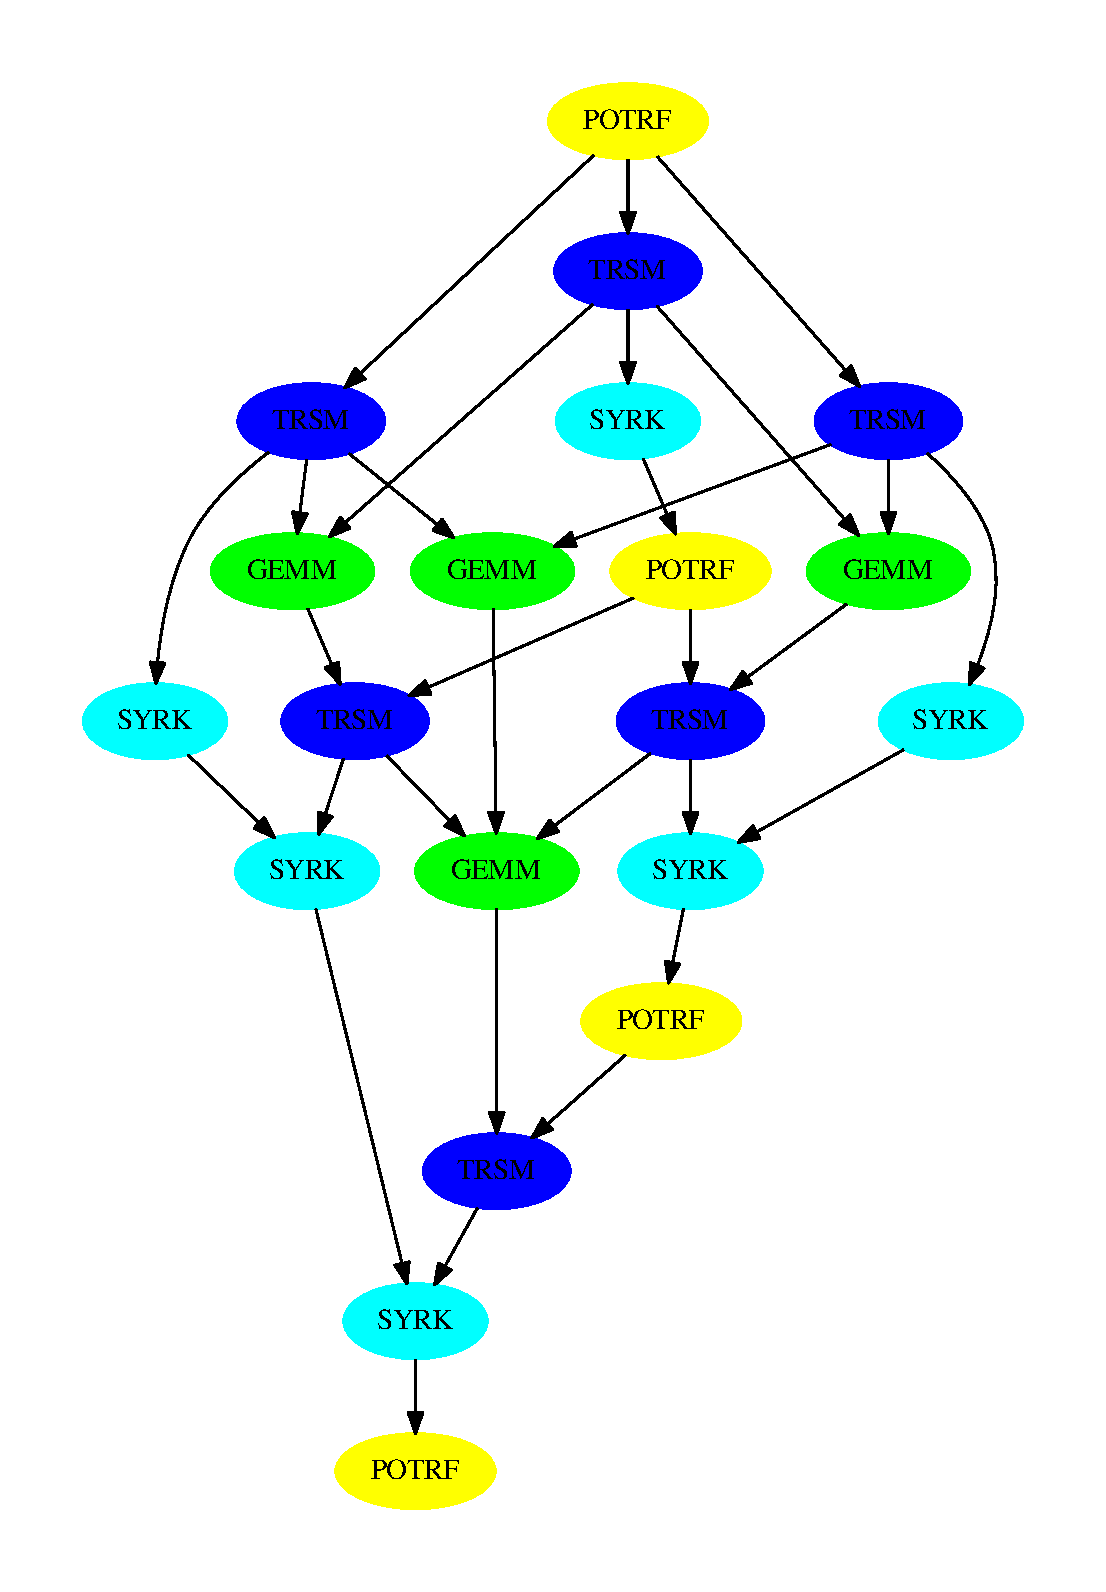
\includegraphics[scale=0.15]{./diagrams/choleskyWithoutId_4.pdf}
%%%%	\end{center}
%%%%\end{exampleblock}
%%%%}\end{minipage}\hfill
%%%%\begin{minipage}{0.525\linewidth}{\footnotesize
%%%%\begin{block}{StarPU scheduler performance}
%%%%		\begin{center}
%%%%	\includegraphics[scale=0.425]{./diagrams/Actual_vs_GEMMBound.eps}	
%%%%		\end{center}
%%%%\end{block}\vspace*{-0.25cm}
%%%%	\begin{block}{}{\footnotesize
%%%%		\begin{itemize}
%%%%			\item A heterogeneous platform with 9 CPUs and 3 GPUs
%%%%			\item StarPU scheduler is based on popular heft strategy
%%%%%%			\item Goal: propose approaches to enhance performance bounds and better scheduling strategies
%%%%		\end{itemize}
%%%%		%%		$\bullet$Goal: Propose approaches to enhance performance bounds and better scheduling strategies
%%%%		%%	\begin{itemize}
%%%%		%%		\item Propose approaches to enhance performance bounds
%%%%		%%		\item Propose better scheduling strategies
%%%%		%%	\end{itemize}
%%%%}\end{block}
%%%%}\end{minipage}
%%%%\vspace*{-0.15cm}
%%%%\begin{block}{}{\footnotesize
%%%%	\begin{itemize}
%%%%%%		\item A heterogeneous platform with 9 CPUs and 3 GPUs
%%%%%%		\item StarPU scheduler is based on popular heft strategy
%%%%		\item Goal: propose approaches to enhance performance bounds and better scheduling strategies
%%%%	\end{itemize}
%%%%\noindent {\scriptsize Joint work with E. Agullo, O. Beaumont, L. Eyraud-Dubois, and S. Thibault during my PhD at Inria Bordeaux}
%%%%	%%		$\bullet$Goal: Propose approaches to enhance performance bounds and better scheduling strategies
%%%%	%%	\begin{itemize}
%%%%	%%		\item Propose approaches to enhance performance bounds
%%%%	%%		\item Propose better scheduling strategies
%%%%	%%	\end{itemize}
%%%%}\end{block}
%%%%\end{frame}

%%\begin{frame}{Iterative Performance Bound}
%%\begin{columns}
%%	\begin{column}[c]{.475\linewidth}
%%		\begin{block}{\centering {\scriptsize DAG}}
%%			\only<1-3> {\centering \includegraphics[scale=0.25]{boundsDiagram/taskgraph}}
%%			%\only<2-3> {\centering 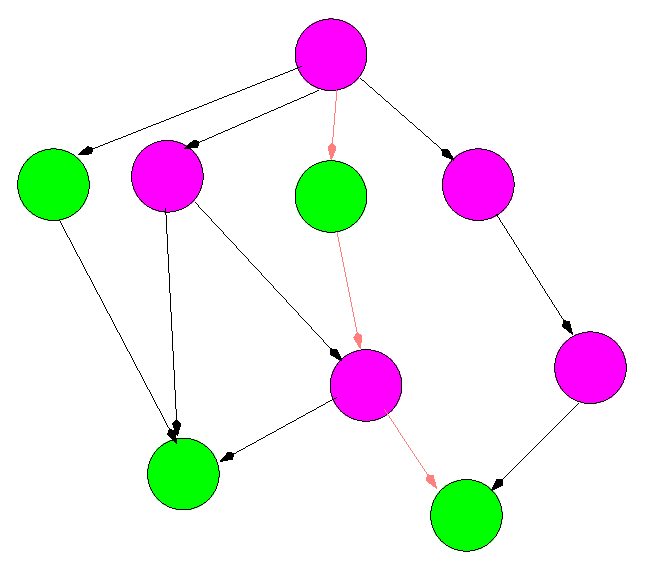
\includegraphics[scale=0.25]{boundsDiagram/taskgraphPath}}
%%		\end{block}
%%	\end{column}\hfill
%%	\begin{column}[c]{.475\linewidth}
%%		\begin{block}{\centering {\scriptsize \only<1> {No} \only<2-3> {Some} 
%%					Dependencies}}
%%			\only<1> {\centering \includegraphics[scale=0.25]{boundsDiagram/taskgraphNoDep}}
%%			\only<2-3> {\centering \includegraphics[scale=0.25]{boundsDiagram/taskgraphOnePath}}
%%		\end{block}
%%	\end{column}
%%\end{columns}
%%\begin{block}{\centering {\scriptsize Minimum execution time (minimize \textit{l})}}
%%	\begin{columns}
%%		\begin{column}[c]{.5\linewidth}
%%			\centering \includegraphics[scale=0.45]{boundsDiagram/schedule}   
%%		\end{column}
%%		\begin{column}[c]{.5\linewidth}
%%			\only<2-3>
%%			{
%%				\begin{itemize}
%%					\item[$\star$]{\scriptsize If any path in DAG is larger than \textit{l}}
%%					\only<3>{
%%						\begin{itemize}
%%							\item {\scriptsize add this path as a constraint and repeat the procedure}
%%						\end{itemize}
%%					}
%%				\end{itemize}
%%			}
%%			
%%		\end{column}  
%%	\end{columns}
%%\end{block}
%%
%%\end{frame}
%%
%%\begin{frame}{Comparison of Simulated Performance and Bounds}
%%\begin{center}
%%	\includegraphics[scale=0.8]{./diagrams/boundsVsSimulation}
%%\end{center}
%%\end{frame}



%%\begin{frame}{Scheduling strategies}
%%
%%{\footnotesize
%%%%\begin{itemize}
%%%%	\item Decide based on current state of resources
%%%%\end{itemize}
%%\vspace*{-0.1cm}
%%\begin{block}{Heft Scheduler [Topcuoglu et al., 2002]}
%%\begin{itemize}
%%	\item Task centric scheduler and based on heterogeneous early finish time heuristic
%%	%\item Based on minimum completion time (MCT) heuristic 
%%%%	\item Based on Heterogeneous early finish time heuristic
%%	%\item Similar to StarPU dmdas scheduler
%%\end{itemize}
%%	\begin{columns}
%%		\begin{column}[c]{.5\linewidth}
%%			\begin{itemize}
%%				\item $A$ is highest priority ready task at $t$ 
%%				\item Completion time on resource2 is minimum
%%				\item Task $A$ is assigned to resource2
%%			\end{itemize}
%%		\end{column}
%%		\begin{column}[c]{.5\linewidth}
%%			\centering \includegraphics[scale=0.325]{basicSchedulers/heftp1} 
%%			\centering \includegraphics[scale=0.325]{basicSchedulers/heftp2}
%%		\end{column}
%%	\end{columns}
%%\end{block}
%%\vspace*{-0.1cm}
%%\begin{block}{\heteroprio Scheduler [Agullo et al., 2016]}
%%\begin{itemize}
%%	\item Resource centric scheduler and based on tasks heterogeneity factors   
%%%%	\item Suitable for a large set of small independent tasks 
%%\end{itemize}
%%	\begin{columns}
%%	\begin{column}[c]{.5\linewidth}
%%		\begin{itemize}
%%			\item $A$ is highest priority ready task at $t$
%%			\item Resource1 is best suited to task $C$
%%			\item Resource1 selects task $C$
%%		\end{itemize}
%%	\end{column}
%%	\begin{column}[c]{.5\linewidth}
%%		\centering \includegraphics[scale=0.325]{basicSchedulers/heteroprio1} 
%%		\centering \includegraphics[scale=0.325]{basicSchedulers/heteroprio2}
%%	\end{column}
%%\end{columns}
%%\end{block}
%%
%%}
%%\end{frame}
%%
%%\begin{frame}{\heteroprio Scheduler}
%%
%%{\footnotesize
%%\begin{block}{}
%%\begin{columns}
%%	\begin{column}[c]{.5\linewidth}
%%	\begin{itemize}
%%%%		\item $A$ is highest priority ready task at $t$
%%%%		\item Resource1 is best suited to task $C$
%%		\item Resource2 completes tasks $A$ and $B$
%%		\item $C$ is running on resource1, wchich may be much faster on resource2
%%	\end{itemize}
%%\end{column}
%%\begin{column}[c]{.5\linewidth}
%%	\centering \includegraphics[scale=0.325]{basicSchedulers/heteroprio3} 
%%\end{column}
%%\end{columns}
%%\medskip
%%\begin{itemize}
%%	\item Nothing prevents the slow resource to execute a long task
%%	\item Suitable for small independent tasks
%%\end{itemize}
%%\end{block}
%%
%%
%%\begin{block}{Generalization of \heteroprio}
%%\begin{columns}
%%	\begin{column}[c]{.5\linewidth}
%%		\begin{itemize}
%%			\item Spoliation: An idle resource restarts the highest priority task if it finishes earlier
%%			%%		\item $A$ is highest priority ready task at $t$
%%			%%		\item Resource1 is best suited to task $C$
%%			\item Resource2 spoliates task $C$
%%		\end{itemize}
%%	\end{column}
%%	\begin{column}[c]{.5\linewidth}
%%		\centering \includegraphics[scale=0.325]{basicSchedulers/heteroprio4} 
%%	\end{column}
%%\end{columns}
%%\medskip
%%Other corrections to \heteroprio:
%%\begin{itemize}
%%	\item CPU selects lowest priority task among all tasks of 
%%	same acceleration factor
%%	\item GPU selects highest priority task among all tasks of 
%%	similar acceleration factors
%%\end{itemize}
%%
%%\end{block}
%%}
%%\end{frame}
%%

\begin{frame}{Our strategy and Performance comparison}

{\scriptsize
	\vspace*{-0.195cm}
	\begin{block}{Trace for 12 X 12  tile matrix of Cholesky factorization}
		\vspace*{-0.175cm}\begin{columns}
			\begin{column}{0.475\linewidth}
			\vspace*{-0.15cm}\begin{block}{}
				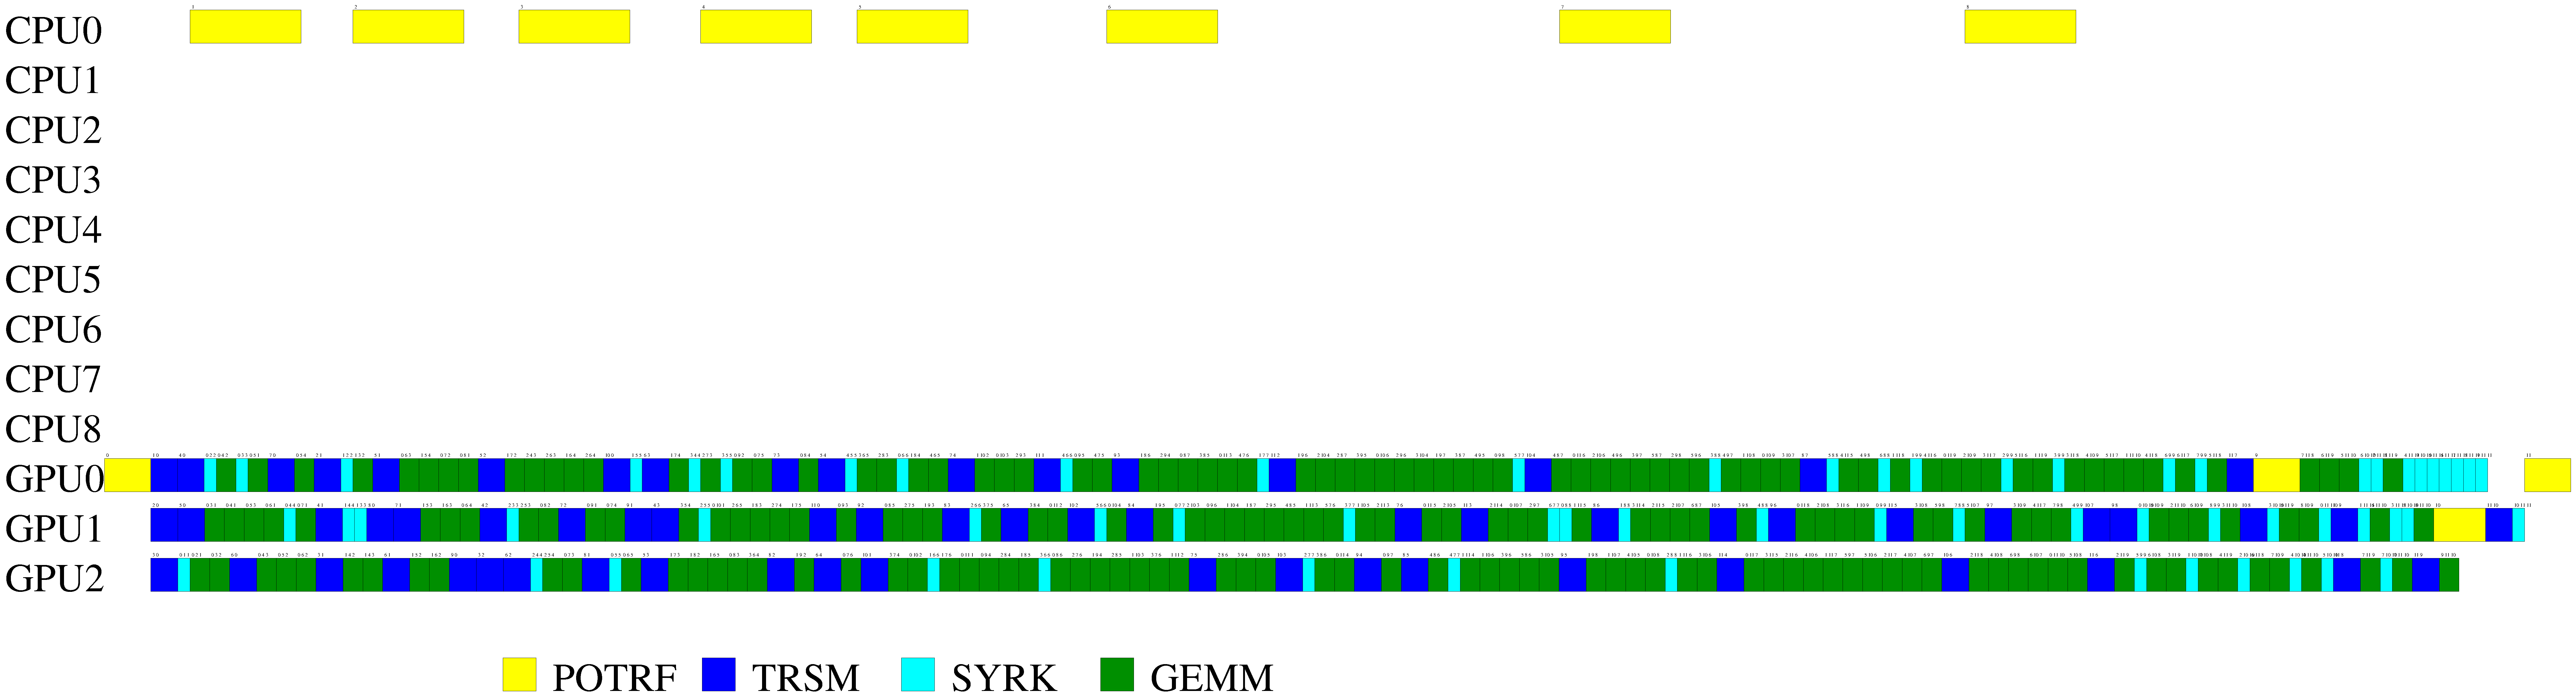
\includegraphics[width=0.925\textwidth,height=0.215\textheight]{./diagrams/heftp-12}\newline\newline
				\noindent StarPU scheduling strategy, performance = 686 GFlop/s \vspace*{-0.045cm}
			\end{block}
			\end{column}
			\begin{column}{0.495\linewidth}
				\vspace*{-0.15cm}\begin{block}{}
				\includegraphics[width=0.925\textwidth,height=0.215\textheight]{./diagrams/heteroprio+PCEPT-12}\\
				\noindent {\tiny \textcolor{blue}{$\bullet$} Resource selects the best suited task \textcolor{blue}{$\bullet$} Fast resource restarts the blocking task}\newline
				\noindent Our strategy, performance = 760 GFlop/s \vspace*{-0.045cm}
				\end{block}
			\end{column}
		\end{columns}	
	\end{block}\vspace*{-0.185cm}
	\begin{block}{Theoretical guarantees of our strategy and performance comparison}\vspace*{-0.35cm}
		\begin{columns}
			\begin{column}{0.45\linewidth}
%%%%				\begin{block}{}
%%%%					\textcolor{blue}{$\bullet$} Each resource selects the best suited task\\
%%%%					\textcolor{blue}{$\bullet$} A fast resource restarts the blocking task
%%%%				\end{block}
%%%%				\vspace*{-0.1cm}
\begin{block}{}
				\setlength{\tabcolsep}{2pt}
				\begin{center}
					\begin{tabular}{|c|c|c|}
						\hline
						&\multicolumn{2}{|c|}{For a set of independent tasks}\\ \cline{2-3} 
						({\tiny\#CPUs, \#GPUs}) & Approximation ratio & Worst case ex.\\ 
						\hline
						(1,1) & $\frac{1 + \sqrt{5}}{2}$ & $\frac{1 + \sqrt{5}}{2}$\\ \hline
						(m,1) & $\frac{3 + \sqrt{5}}{2}$ & $\frac{3 + \sqrt{5}}{2}$\\ \hline
						(m,n) & $2 + \sqrt{2} \approx 3.41 $ & $2 +
						\frac{2}{\sqrt{3}} \approx 3.15$ \\ \hline
					\end{tabular}
				\end{center}
\end{block}
			\end{column}
			\begin{column}{0.5\linewidth}\vspace*{-0.925cm}
				\begin{center}
					\includegraphics[scale=0.465]{./plots/BoundsVsHeftVsHeteroPrioPerformance}
%%					\includegraphics[width=\textwidth,height=0.3\textheight]{./plots/BoundsVsHeftVsHeteroPrioPerformance}
				\end{center}\vspace*{-1.0cm}
			\noindent $\qquad\qquad$\textcolor{blue}{$\bullet$} Our upper bound is obtained by a linear program\vspace*{-0.045cm}
%%#msize heft hp-best iterativeBound(5mins)
%%4 199.95 204.52 208.01
%%8 522.86 554.40 603.87
%%12 674.93 759.99 835.75
%%16 781.96 857.23 930.31
%%20 843.70 907.50 956.59
%%24 877.75 933.94 966.07
%%28 897.97 951.22 971.79
%%32 914.02 960.19 975.61			
			\end{column}
		\end{columns}
\end{block}
}
\end{frame}


%%%%
%%%%\begin{frame}{Theoretical guarantees of our strategy and performance comparison}
%%%%\begin{minipage}{0.475\linewidth}{\footnotesize
%%%%		\setlength{\tabcolsep}{2pt}
%%%%		\begin{block}{For a set of independent tasks}
%%%%			\begin{center}
%%%%				\begin{tabular}{|c|c|c|}
%%%%					\hline
%%%%					({\tiny\#CPUs, \#GPUs}) & Approximation ratio & Worst case ex.\\ 
%%%%					\hline
%%%%					(1,1) & $\frac{1 + \sqrt{5}}{2}$ & $\frac{1 + \sqrt{5}}{2}$\\ \hline
%%%%					(m,1) & $\frac{3 + \sqrt{5}}{2}$ & $\frac{3 + \sqrt{5}}{2}$\\ \hline
%%%%					(m,n) & $2 + \sqrt{2} \approx 3.41 $ & $2 +
%%%%					\frac{2}{\sqrt{3}} \approx 3.15$ \\ \hline
%%%%				\end{tabular}
%%%%			\end{center}
%%%%		\end{block}
%%%%		\begin{block}{For task graphs}
%%%%			\begin{center}
%%%%				\begin{tabular}{|c|c|c|}
%%%%					\hline
%%%%					({\tiny\#CPUs, \#GPUs}) & Approximation ratio & Worst case ex.\\ 
%%%%					\hline
%%%%					(1,1) & $2$ & $2$\\ \hline
%%%%					(m,n) & $2 + \max(\frac{m}{n}, \frac{n}{m})$ & $1 + \max(\frac{m}{n}, \frac{n}{m})$\\ \hline
%%%%				\end{tabular}
%%%%			\end{center}
%%%%		\end{block}
%%%%}\end{minipage}\hfill
%%%%\begin{minipage}{0.475\linewidth}{\footnotesize
%%%%		\begin{block}{Performance comparison}
%%%%			\begin{center}
%%%%				\includegraphics[scale=0.5]{./plots/BoundsVsHeftVsHeteroPrioPerformance}
%%%%			\end{center}
%%%%			%%\vspace*{-0.25cm}
%%%%			%%\textcolor{blue}{$\bullet$} Iterative bound: obtained by adding longest path iteratively in a linear program
%%%%		\end{block}
%%%%}\end{minipage}
%%%%\begin{itemize}
%%%%	\item Iterative bound is obtained by adding longest path iteratively in a linear program
%%%%	\item Performance of our strategy is close to the bound
%%%%\end{itemize}
%%%%\end{frame}
%%%%


%%\begin{frame}{Trace for 12 X 12  blocks of Cholesky factorization}
%%
%%{\scriptsize
%%\vspace*{-0.15cm}
%%\begin{block}{StarPU scheduling strategy}
%%
%%	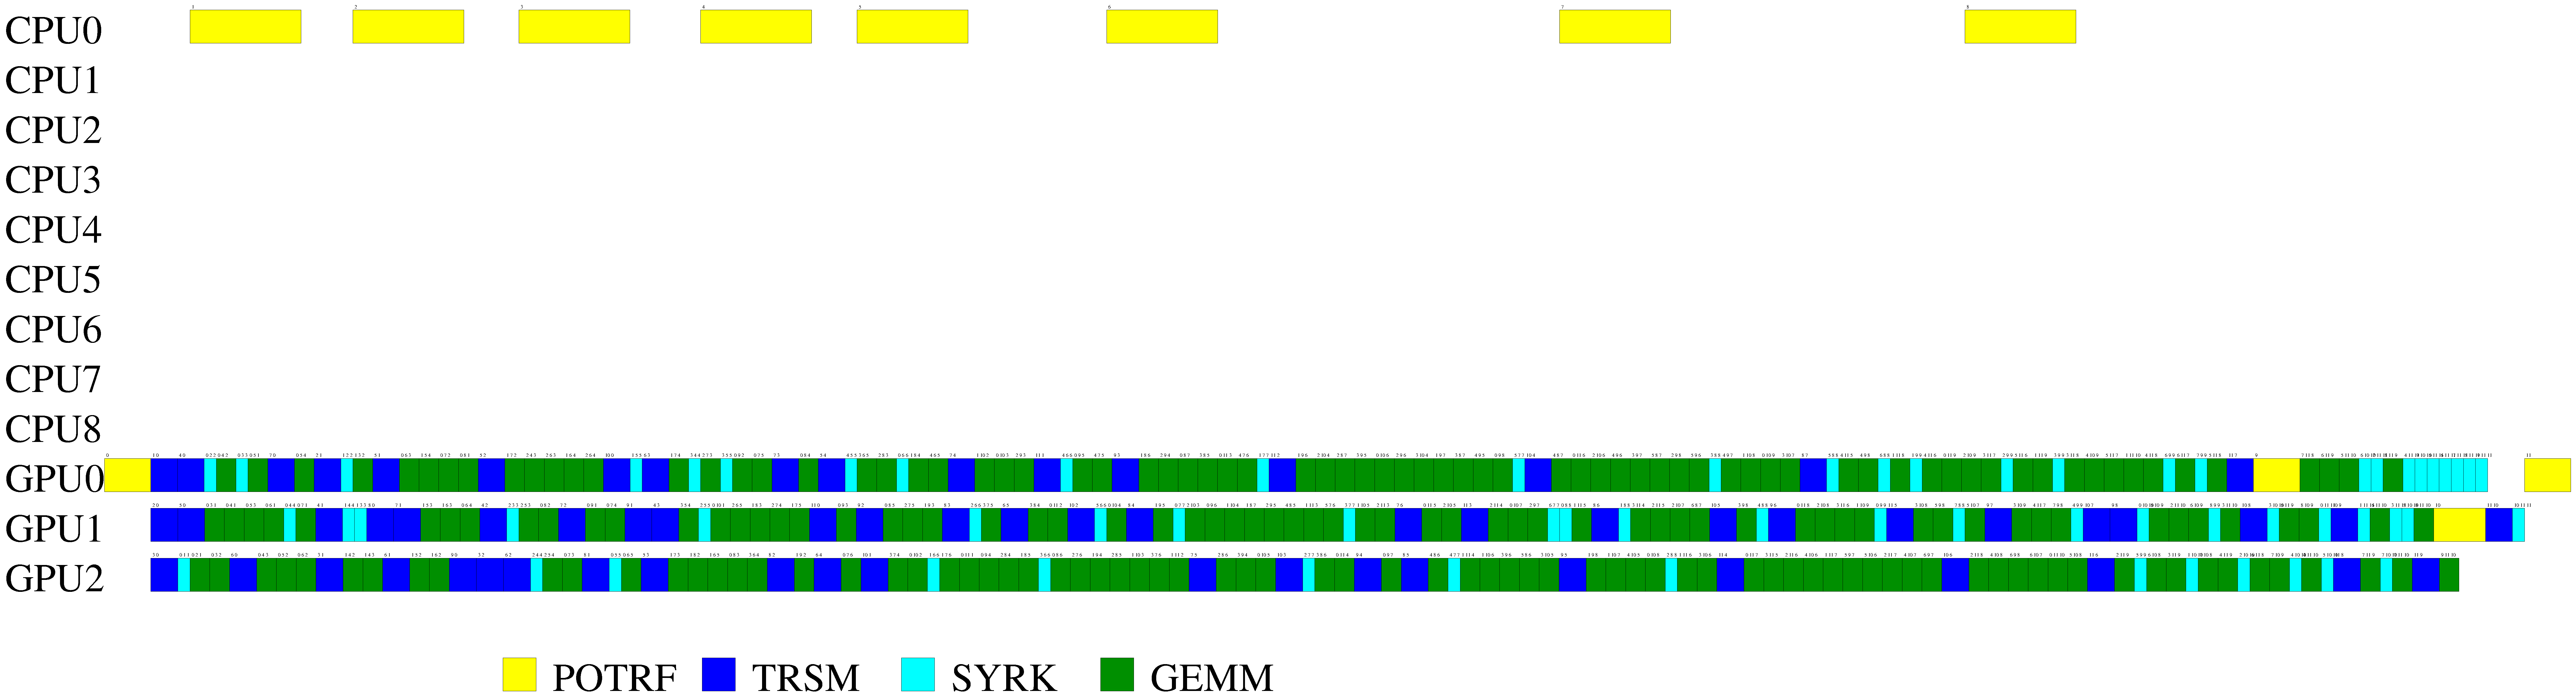
\includegraphics[width=0.475\textwidth,height=0.225\textheight]{./diagrams/heftp-12}
%%
%%\noindent Achieved performance = 686 GFlop/s
%%
%%\end{block}
%%\vspace*{-0.25cm}
%%\begin{block}{Our scheduling strategy}
%%%%\begin{center}
%%\includegraphics[width=0.45\textwidth,height=0.225\textheight]{./diagrams/heteroprio+PCEPT-12}
%%%%\end{center}
%%\vspace*{-0.15cm}
%%\begin{block}{}
%%	\textcolor{blue}{$\bullet$} Each resource selects the best suited task\\
%%	\textcolor{blue}{$\bullet$} An idle resource restarts the highest priority task if it finishes earlier
%%\end{block}
%%\vspace*{-0.1cm}
%%\noindent Achieved performance = 760 GFlop/s
%%\end{block}
%%}
%%\end{frame}



%%\begin{frame}{Trace for 12 X 12  blocks of Cholesky with StarPU scheduling strategy}
%%%%\framesubtitle{Trace for 12 X 12  blocks of Cholesky factorization with StarPU scheduling strategy}
%%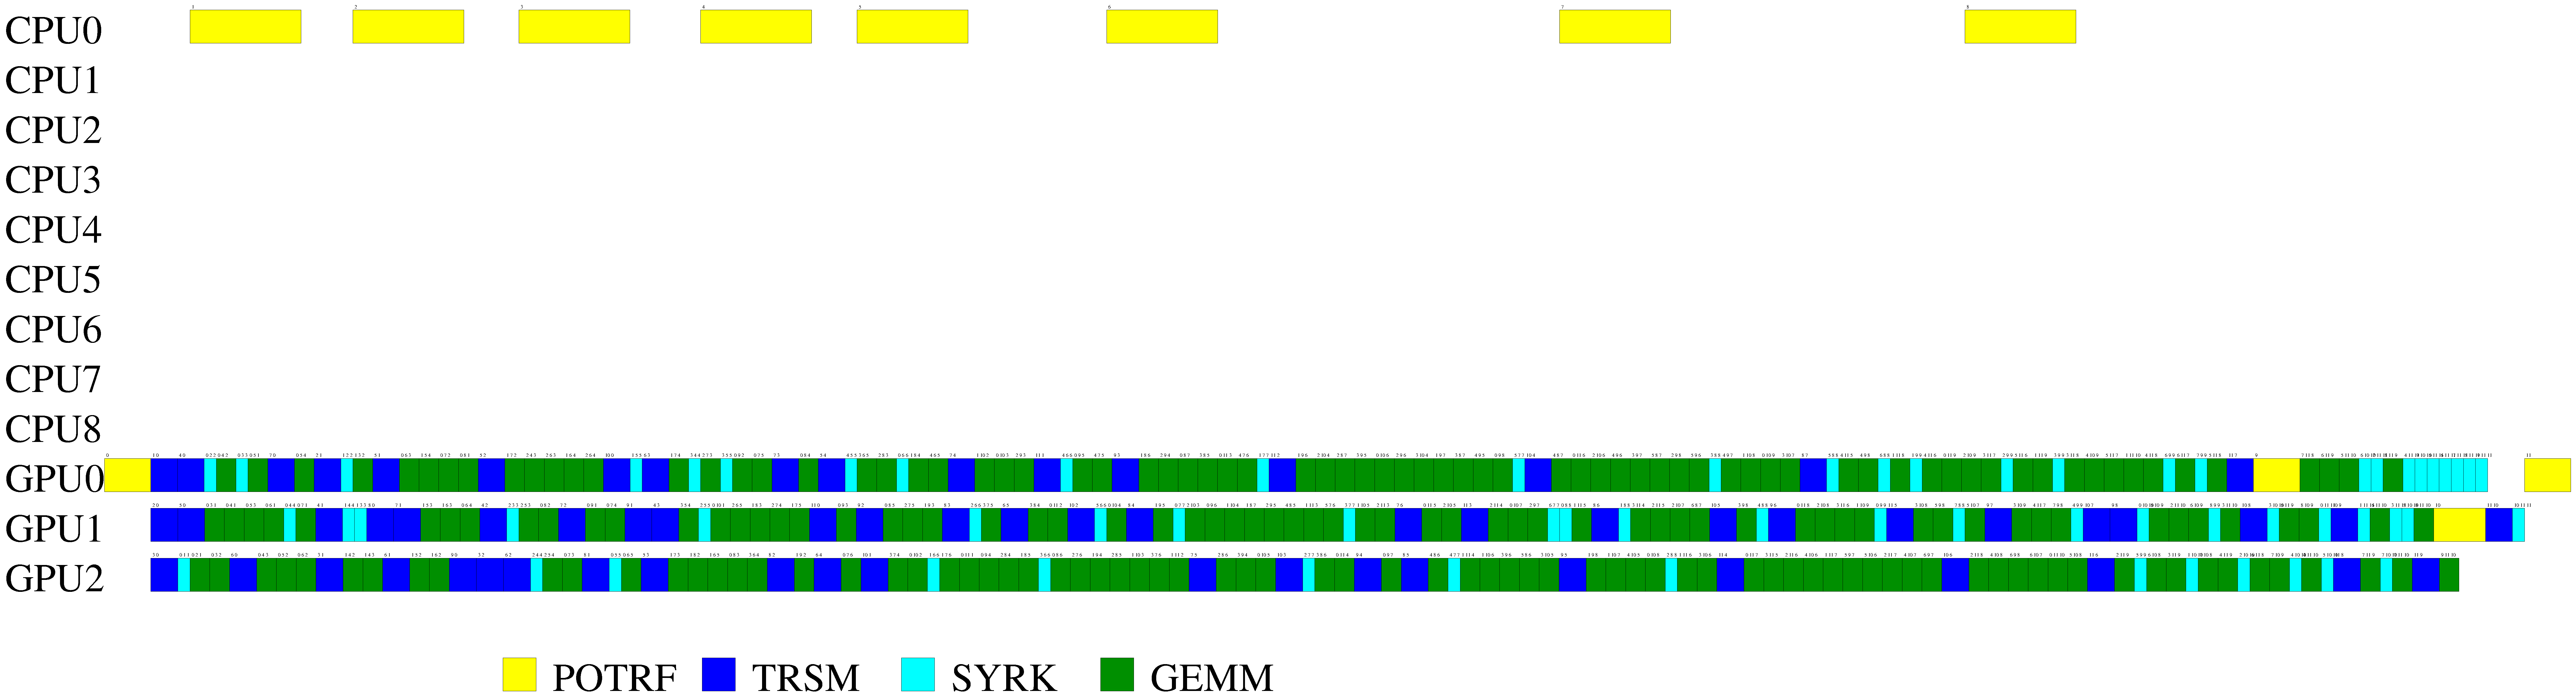
\includegraphics[width=\textwidth,height=0.72\textheight]{./diagrams/heftp-12}
%%\vspace*{-0.25cm}
%%\begin{itemize}
%%\item Most of the CPU resources are not utilized (686 GFlop/s)
%%%%\item SS performance = 791 GFlop/s
%%\end{itemize}
%%\end{frame}
%%
%%
%%
%%
%%
%%\begin{frame}{Trace for 12 X 12  blocks of Cholesky with our scheduling strategy}
%%\includegraphics[width=\textwidth,height=0.625\textheight]{./diagrams/heteroprio+PCEPT-12}
%%
%%%%\only<1>{\includegraphics[width=\textwidth,height=0.725\textheight]{./diagrams/heteroprio+PCEPT-12}\vspace*{-0.25cm}}
%%%%\only<2>{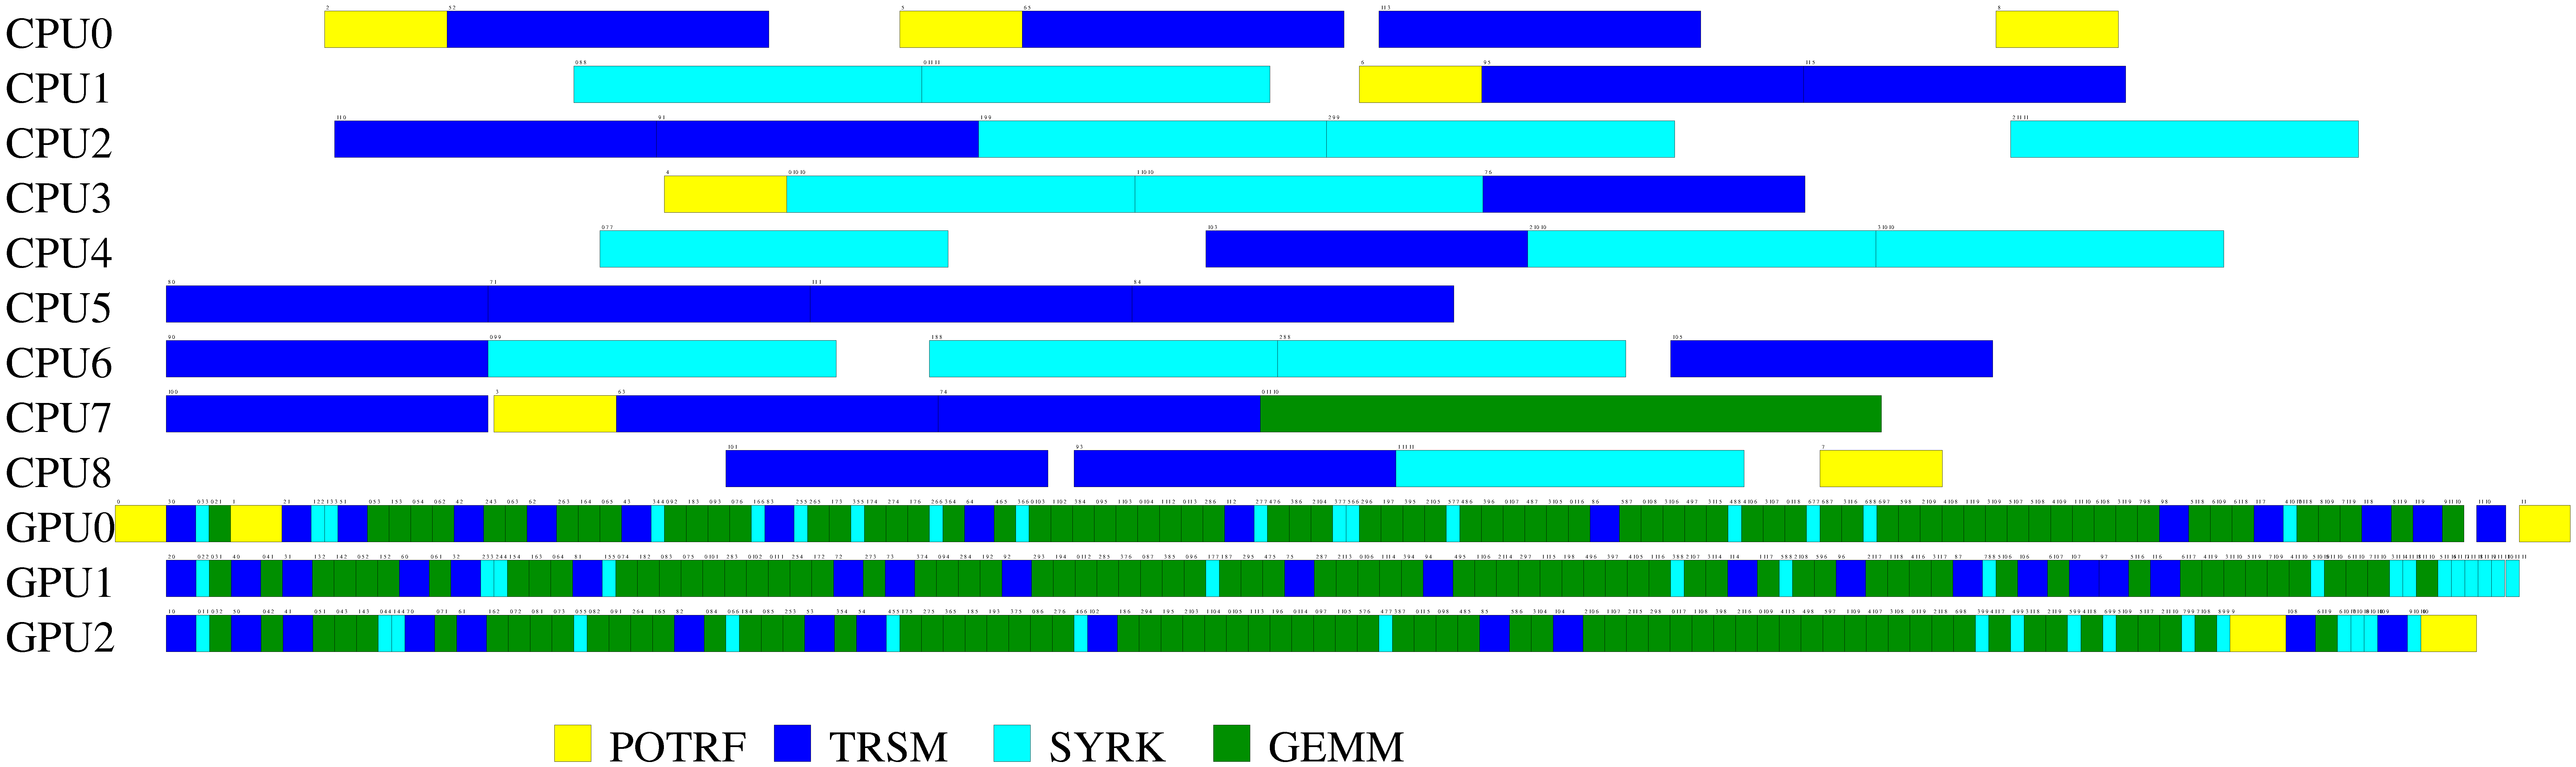
\includegraphics[width=\textwidth,height=0.725\textheight]{./diagrams/HP+PCEPTWithoutAbortedTasks}}
%%\vspace*{-0.15cm}
%%\begin{block}{}
%%\textcolor{blue}{$\bullet$} Each resource selects the best suited task\\
%%\textcolor{blue}{$\bullet$} An idle resource restarts the highest priority task if it finishes earlier
%%\end{block}
%%\vspace*{-0.185cm}
%%Achieved performance = 760 GFlop/s, Performance with StarPU strategy = 686 GFlop/s
%%\end{frame}

%%%%
%%%%\begin{frame}{Theoretical guarantees of our strategy and performance comparison}
%%%%\begin{minipage}{0.475\linewidth}{\footnotesize
%%%%\setlength{\tabcolsep}{2pt}
%%%%\begin{block}{For a set of independent tasks}
%%%%\begin{center}
%%%%	\begin{tabular}{|c|c|c|}
%%%%		\hline
%%%%		({\tiny\#CPUs, \#GPUs}) & Approximation ratio & Worst case ex.\\ 
%%%%		\hline
%%%%		(1,1) & $\frac{1 + \sqrt{5}}{2}$ & $\frac{1 + \sqrt{5}}{2}$\\ \hline
%%%%		(m,1) & $\frac{3 + \sqrt{5}}{2}$ & $\frac{3 + \sqrt{5}}{2}$\\ \hline
%%%%		(m,n) & $2 + \sqrt{2} \approx 3.41 $ & $2 +
%%%%		\frac{2}{\sqrt{3}} \approx 3.15$ \\ \hline
%%%%	\end{tabular}
%%%%\end{center}
%%%%\end{block}
%%%%\begin{block}{For task graphs}
%%%%	\begin{center}
%%%%		\begin{tabular}{|c|c|c|}
%%%%			\hline
%%%%			({\tiny\#CPUs, \#GPUs}) & Approximation ratio & Worst case ex.\\ 
%%%%			\hline
%%%%			(1,1) & $2$ & $2$\\ \hline
%%%%			(m,n) & $2 + \max(\frac{m}{n}, \frac{n}{m})$ & $1 + \max(\frac{m}{n}, \frac{n}{m})$\\ \hline
%%%%		\end{tabular}
%%%%	\end{center}
%%%%
%%%%%%\begin{center}
%%%%%%	\begin{tabular}{|c|c|c|c|c|}
%%%%%%		\hline
%%%%%%		&\multicolumn{2}{|c|}{set of independent tasks} &\multicolumn{2}{|c|}{task graphs}\\ \cline{2-5}
%%%%%%		(\#CPUs, \#GPUs) & Approximation ratio & Worst case ex. & Approximation ratio & Worst case ex.\\ 
%%%%%%		\hline
%%%%%%		(1,1) & $\frac{1 + \sqrt{5}}{2}$ & $\frac{1 + \sqrt{5}}{2}$ & 2 & 2\\ \hline
%%%%%%		%			(1,n) & $2$ \\ \hline
%%%%%%		%%		(m,1) & $\frac{3 + \sqrt{5}}{2}$ & $\frac{3 + \sqrt{5}}{2}$\\ \hline
%%%%%%		%			(m,n) \& $m \le n-1$ & $3$ \\ \hline
%%%%%%		%			(m,n) & $2 + \sqrt{2} \approx 3.41 $ &  $3$\\ \hline
%%%%%%		(m,n) & $2 + \sqrt{2} \approx 3.41 $ & $2 +
%%%%%%		\frac{2}{\sqrt{3}} \approx 3.15$ & $2 + \max(\frac{m}{n}, \frac{n}{m})$ & $1 + \max(\frac{m}{n}, \frac{n}{m}) $\\ \hline
%%%%%%	\end{tabular}
%%%%%%\end{center}
%%%%\end{block}
%%%%}\end{minipage}\hfill
%%%%\begin{minipage}{0.475\linewidth}{\footnotesize
%%%%	\begin{block}{Performance comparison}
%%%%\begin{center}
%%%%	\includegraphics[scale=0.5]{./plots/BoundsVsHeftVsHeteroPrioPerformance}
%%%%\end{center}
%%%%%%\vspace*{-0.25cm}
%%%%%%\textcolor{blue}{$\bullet$} Iterative bound: obtained by adding longest path iteratively in a linear program
%%%%	\end{block}
%%%%}\end{minipage}
%%%%\begin{itemize}
%%%%	\item Iterative bound is obtained by adding longest path iteratively in a linear program
%%%%	\item Performance of our strategy is close to the bound
%%%%\end{itemize}
%%%%\end{frame}


%%\subsection{Communication Computation Overlap}
%%\begin{frame}
%%\frametitle{Previous Activities}
%%\tableofcontents[currentsubsection]
%%\end{frame}

\section{Minimize Impact of Data Transfers on Large Scale Systems}

\begin{frame}{Minimizing impact of communications on Summit supercomputer}
\begin{itemize}{\footnotesize
\item Maximizing the overlap of communications and computations
\item Implemented proposed approaches in Tensor Algebra for Manybody Methods (TAMM) library
\item Molecular chemistry application (CCSD), Ubiqtin molecule, cc-pVDZ (737 basis functions, 220 nodes), aug-cc-pVDZ (1243 basis functions, 256 nodes)
}\end{itemize}
\begin{columns}
\begin{column}{0.56\linewidth}
\begin{center}\vspace*{-0.325cm}
\includegraphics[scale=0.115]{./diagrams/Summit_Node.jpg}
\end{center}
\vspace*{-0.4cm}{\tiny Joint work with S. Krishnamoorthy and M. Zalewski during my postdoc at PNNL, USA}
{\tiny Figure source: \url{https://www.olcf.ornl.gov}}
\end{column}
\begin{column}{0.45\linewidth}
\includegraphics[scale=0.5]{./diagrams/tamm-performance.eps}
\end{column}
\end{columns}
\end{frame}



\part[Proposed Plan]{Proposed Plan}
\begin{frame}{Project: Scalable Tensor Algorithms for Modern Computing Systems}
\frametitle{} % Table of contents slide, comment this block out to remove it
\tableofcontents[part=2] % Throughout your presentation, if you choose to use \section{} and \subsection{} commands, these will automatically be printed on this slide as an overview of your presentation

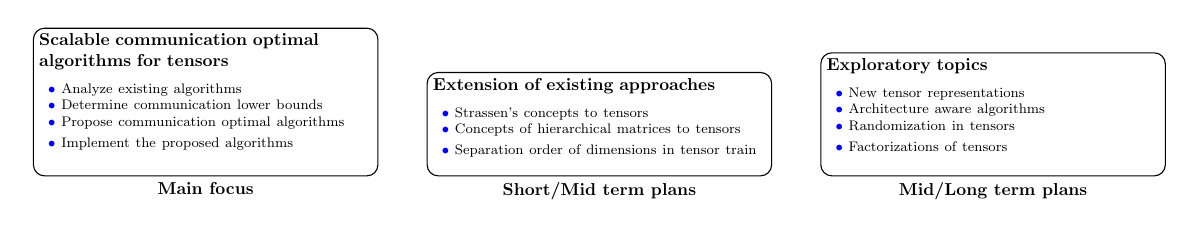
\begin{tikzpicture}[scale=0.625, every node/.style={transform shape}]
\tikzstyle{taskr}=[draw=black, rounded corners, minimum height=30mm, minimum width=70mm, fill=none, text=black]


%%\tikzstyle{taskcompute}=[draw=black, minimum height=16mm, minimum width=16mm, fill=none, text=black, below]


\node (mainfocus) at (0,0) [taskr, anchor=south] {};
\node at (mainfocus.south) [below] {\textbf{Main focus}};

\node [below, align=left, text width=70mm]at (mainfocus.north) {		\textbf{$\ $Scalable communication optimal\\ $\ $algorithms for tensors\medskip}\\{\footnotesize \mybullet Analyze existing algorithms\\ 
		\mybullet Determine communication lower bounds\\\mybullet Propose communication optimal algorithms\\\mybullet Implement the proposed algorithms}};


\node (shorttermfocus) at (8,0) [taskr, minimum height=21mm, anchor=south] {};
\node at (shorttermfocus.south) [below] {\textbf{Short/Mid term plans}};

\node [below, align=left, text width=70mm]at (shorttermfocus.north) {\textbf{$\ $Extension of existing approaches\medskip}\\\footnotesize \mybullet Strassen's concepts to tensors\\\mybullet Concepts of hierarchical matrices to tensors\\\mybullet Separation order of dimensions in tensor train};


\node (midtermfocus) at (16,0) [taskr, minimum height=25mm, anchor=south] {};
\node at (midtermfocus.south) [below] {\textbf{Mid/Long term plans}};

\node [below, align=left, text width=70mm]at (midtermfocus.north) {\textbf{$\ $Exploratory topics\medskip}\\\footnotesize \mybullet New tensor representations\\ \mybullet Architecture aware algorithms\\ \mybullet Randomization in tensors\\ \mybullet Factorizations of tensors};

\end{tikzpicture}

\end{frame}


%%%%\begin{frame}{Test}
%%%%\begin{tikzpicture}[scale=0.625, every node/.style={transform shape}]
%%%%\tikzstyle{taskr}=[draw=black, rounded corners, minimum height=30mm, minimum width=70mm, fill=none, text=black]
%%%%
%%%%
%%%%%%\tikzstyle{taskcompute}=[draw=black, minimum height=16mm, minimum width=16mm, fill=none, text=black, below]
%%%%
%%%%
%%%%\node (mainfocus) at (0,0) [taskr, anchor=south] {};
%%%%\node at (mainfocus.south) [below] {\textbf{Main Focus}};
%%%%
%%%%\node [below, align=left, text width=70mm]at (mainfocus.north) {		\textbf{$\ $Scalable communication optimal algorithms for tensors}\\{\footnotesize \mybullet Analyze existing algorithms\\ 
%%%%		\mybullet Determine communication lower bounds\\\mybullet Propose communication optimal algorithms\\\mybullet Implement the proposed algorithms}};
%%%%
%%%%
%%%%\node (shorttermfocus) at (8,0) [taskr, minimum height=15mm, anchor=south] {};
%%%%\node at (shorttermfocus.south) [below] {\textbf{Short term plans}};
%%%%
%%%%\node [below, align=left, text width=70mm]at (shorttermfocus.north) {\footnotesize \mybullet Extend Strassen's concepts to tensors\\\mybullet Extend hierarchical matrices to tensors\\\mybullet Separation order of dimensions in tensor train};
%%%%
%%%%
%%%%\node (midtermfocus) at (16,0) [taskr, minimum height=20mm, anchor=south] {};
%%%%\node at (midtermfocus.south) [below] {\textbf{Mid term plans}};
%%%%
%%%%\node [below, align=left, text width=70mm]at (midtermfocus.north) {\footnotesize \mybullet New tensor representations\\ \mybullet Architecture aware algorithms\\ \mybullet Randomization in tensors\\ \mybullet Factorizations of tensors};
%%%%
%%%%
%%%%%%		\textbf{Scalable communication optimal algorithms for tensors}\\{\footnotesize $\quad$Analyze existing algorithms\\ 
%%%%%%		$\quad$Determine communication lower bounds\\$\quad$Propose communication optimal algorithms\\$\quad$Implement the proposed algorithms}};
%%%%
%%%%
%%%%
%%%%%%		\\Determine communication lower bounds\\Propose communication optimal algorithms\\Implement the proposed algorithms}};
%%%%
%%%%%%		\node (textmainfocus) at (mainfocus.south) [below] {Scalable communication optimal algorithms for tensors};
%%%%%%%%%%		\textbf{}}
%%%%\end{tikzpicture}
%%%%\end{frame}






%%\section{Communication and its importance in HPC}
\begin{frame}{Communication and its importance in HPC}

\begin{minipage}{0.6\linewidth}
\begin{itemize}
	\item Running time of an algorithm depends on 
	\begin{itemize}
		\item Computations
		\begin{itemize}
			\item Number of operations * time-per-operation
		\end{itemize}
		\item Data movement
		\begin{itemize}
			\item Volume of communication / Network-bandwidth
			\item Number of messages * Network-latency
		\end{itemize}
	\end{itemize}
\end{itemize}
\end{minipage}
\begin{minipage}{0.35\linewidth}
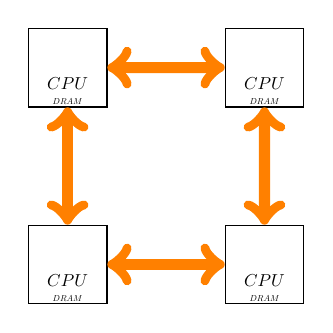
\begin{tikzpicture}[scale=0.625, every node/.style={transform shape}]
%%\tikzstyle{taskmemory}=[draw=black, minimum height=18mm, minimum width=18mm, fill=blue!40, text=black]
\tikzstyle{taskcompute}=[draw=black, minimum height=16mm, minimum width=16mm, fill=none, text=black, below]

\node (t0) at (0,0) [taskcompute] {}; 
\node (t1) at (4,0) [taskcompute] {};
\node (t2) at (4,4) [taskcompute] {};
\node (t3) at (0,4) [taskcompute] {};

\draw [<->, line width=4, orange] (t0) -- (t1);
\draw [<->, line width=4, orange] (t1) -- (t2);
\draw [<->, line width=4, orange] (t2) -- (t3);
\draw [<->, line width=4, orange] (t3) -- (t0);

\node (td0)  at (t0.south) [above, scale=0.5] {$DRAM$};
\node (td1) [above, scale=0.5] at (t1.south) {$DRAM$};
\node (td2) [above, scale=0.5] at (t2.south) {$DRAM$};
\node (td3) [above, scale=0.5] at (t3.south) {$DRAM$};

\node [above] at (td0.north) {$CPU$};
\node [above] at (td1.north) {$CPU$};
\node [above] at (td2.north) {$CPU$};
\node [above] at (td3.north) {$CPU$};

%%\node [below] at (tm.south) {Memory Unit $M$};
%%\node [above] at (tc.north) {Compute Unit $C$};
%%
%%\node [taskmemory, minimum height=6mm, minimum width=12mm, anchor=south] at (tc.south) {}; 
\end{tikzpicture}
\end{minipage}
\begin{itemize}
	\item Gaps growing exponentially with time (Source: Getting up to speed: The future of supercomputing)
		\begin{center}
	\begin{tabular}{|c|c|c|c|}
		\hline
		& time-per-operation & Network-bandwidth & Network-latency\\ \hline
		Annual improvements & 59 \% & 26 \% & 15 \%\\ \hline
%%		\multicolumn{2}{|c|}{Annual improvements}\\ \hline
%%		time-per-operation & 59\%\\ \hline
%%		Network-bandwidth & 26\%\\ \hline
%%		Network-latency & 15 \% \\ \hline
	\end{tabular}
		\end{center}
	\vfill
	%%\credit{Getting up to speed: The future of supercomputing}
	\item Avoid communication to save time (and energy)
\end{itemize}



%%\includegraphics[scale=0.02]{./tmp/networkTopology.jpg}
%%Source: GETTING UP TO SPEED THE FUTURE OF SUPERCOMPUTING
%%Figures fromGetting up to speed:  The future of supercomputing, 2005,National Academies Press (2004 figure based on data on the period 1988-2002)
\end{frame}

\section{Design of Scalable Communication Optimal Algorithms for Tensors (Main Focus)}
%%\begin{frame}
%%\frametitle{Table of Contents}
%%\tableofcontents[currentsection]
%%\end{frame}

\begin{frame}{Scalabale algorithms for popular tensor operations}
\begin{itemize}
	\item Determine the communication lower bounds for tensor decompositions
	\item Analyse the popular decomposition algorithms and communications performed by them
	\item Propose new scalable communication optimal algorithms
	\begin{itemize}
		\item If possible design tiles/tasks based algorithms
	\end{itemize}
	\item Implement the proposed algorithms
	\begin{itemize}
		\item Handle performance issues for homogeneous systems
		\begin{itemize}
			\item Load balancing
			\item Memory aware approaches
			\item scheduling strategies
		\end{itemize}
	\end{itemize}
	\item Same for manipulation operations of popular tensor representations
	\item Extend implementation for heterogeneous systems (start with Nvidia GPUs based heterogeneous systems)
	\item Create a tensor library
\end{itemize}
\end{frame}



%%\begin{frame}{Tensor Diagram Notations }
%%%%$Tensors are denoted by solid shapes aand number of lines coming out of the shapes denote the dimensions of the tensors.$
%%\\
%%\noindent For example,
%%\begin{center}
%%	\begin{tabular}{ccc}
%%		Dimension & Name &\\
%%		1 & Vector & \begin{tikzpicture}[scale=0.5, every node/.style={transform shape}]
%%		\tikzstyle{taskc}=[circle, draw=black, minimum size=3mm, fill=\tensorcolor]
%%		\node (t01) at (0,0) [taskc]{};
%%		\draw (t01) -- (1,0);
%%		\path (t01) -- (-1,0);
%%		\end{tikzpicture} \\
%%		2 & Matrix & \begin{tikzpicture}[scale=0.5, every node/.style={transform shape}]
%%		\tikzstyle{taskc}=[circle, draw=black, minimum size=3mm, fill=\tensorcolor]
%%		\node (t01) at (0,0) [taskc]{};
%%		\draw (t01) -- (1,0);
%%		\draw (t01) -- (-1,0);
%%		\end{tikzpicture} \\
%%		3 & $3$-dimensional tensor & \begin{tikzpicture}[scale=0.5, every node/.style={transform shape}]
%%		\tikzstyle{taskc}=[circle, draw=black, minimum size=3mm, fill=\tensorcolor]
%%		\node (t01) at (0,0) [taskc]{};
%%		\draw (t01) -- (1,0);
%%		\draw (t01) -- (-1,0);
%%		\draw (t01) -- (0,1);	
%%		%%	\draw[<->,thin] (2, -0.2) -- node[below]{$3$} (4, -0.2);
%%		\end{tikzpicture}\\
%%	\end{tabular}
%%\end{center}

%%Tensors are denoted by solid shapes and number of lines coming out of the shapes denote the dimensions of the tensors.

%%\begin{itemize}
%%	\item Connecting two lines implies summation over the connected dimensions
%%	\item Multiplication of matrices \begin{tikzpicture}[scale=0.5, every node/.style={transform shape}]
%%	\tikzstyle{taskc}=[circle, draw=black, minimum size=5mm, fill=\tensorcolor]
%%	\node (t01) at (0,0) [taskc]{A};
%%	%%	\node [below] at (t01.south) {A};
%%	\draw (t01) -- node[above]{j}(1,0);
%%	\draw (t01) -- node[above]{i}(-1,0);
%%	%%	\draw (t01) -- (0,1);	
%%	%%	\draw[<->,thin] (2, -0.2) -- node[below]{$3$} (4, -0.2);
%%	\end{tikzpicture} and
%%	\begin{tikzpicture}[scale=0.5, every node/.style={transform shape}]
%%	\tikzstyle{taskc}=[circle, draw=black, minimum size=5mm, fill=\tensorcolor]
%%	\node (t01) at (0,0) [taskc]{B};
%%	%%	\node [below] at (t01.south) {A};
%%	\draw (t01) -- node[above]{k}(1,0);
%%	\draw (t01) -- node[above]{j}(-1,0);
%%	%%	\draw (t01) -- (0,1);	
%%	%%	\draw[<->,thin] (2, -0.2) -- node[below]{$3$} (4, -0.2);
%%	\end{tikzpicture} is represented as 
%%	\begin{tikzpicture}[scale=0.5, every node/.style={transform shape}]
%%	\tikzstyle{taskc}=[circle, draw=black, minimum size=5mm, fill=\tensorcolor]
%%	\node (t01) at (0,0) [taskc]{C};
%%	%%	\node [below] at (t01.south) {A};
%%	\draw (t01) -- node[above]{k}(1,0);
%%	\draw (t01) -- node[above]{i}(-1,0);
%%	%%	\draw (t01) -- (0,1);	
%%	%%	\draw[<->,thin] (2, -0.2) -- node[below]{$3$} (4, -0.2);
%%	\end{tikzpicture}
%%	=
%%	\begin{tikzpicture}[scale=0.5, every node/.style={transform shape}]
%%	\tikzstyle{taskc}=[circle, draw=black, minimum size=5mm, fill=\tensorcolor]
%%	\node (t01) at (0,0) [taskc]{A};
%%	%%	\node [below] at (t01.south) {A};
%%	%%	\draw (t01) -- node[above]{j}(1,0);
%%	\draw (t01) -- node[above]{i}(-1,0);
%%	
%%	\node (t02) at (2,0) [taskc]{B};
%%	%%	\node [below] at (t01.south) {A};
%%	\draw (t02) -- node[above]{k}(3,0);
%%	\draw (t01) -- node[above]{j}(t02);
%%	%%	\draw (t01) -- (0,1);	
%%	%%	\draw[<->,thin] (2, -0.2) -- node[below]{$3$} (4, -0.2);
%%	\end{tikzpicture}
%%	%%	\vfill
%%	
%%\end{itemize}
%%\end{frame}



\begin{frame}{Popular tensor decompositions}

{\footnotesize\vspace*{-0.175cm}
\begin{block}{Tucker decomposition}
\begin{minipage}{0.325\linewidth}
	\begin{center}
		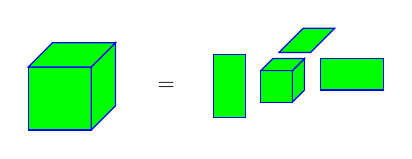
\begin{tikzpicture}[scale=0.2, every node/.style={transform shape}]
		\pgfmathsetmacro{\cubex}{4}
		\pgfmathsetmacro{\cubey}{4}
		\pgfmathsetmacro{\cubez}{4}
		\draw[blue,fill=pastelgreen] (-12,1,\cubez-2) -- ++(-\cubex,0,0) -- ++(0,-\cubey,0) -- ++(\cubex,0,0) -- cycle;
		\draw[blue,fill=pastelgreen] (-12,1,\cubez-2) -- ++(0,0,-\cubez) -- ++(0,-\cubey,0) -- ++(0,0,\cubez) -- cycle;
		\draw[blue,fill=pastelgreen] (-12,1,\cubez-2) -- ++(-\cubex,0,0) -- ++(0,0,-\cubez) -- ++(\cubex,0,0) -- cycle;
		\node[draw=none, text=black, scale=4] at (-8,-1,0) {$=$};
		
		\pgfmathsetmacro{\cubex}{2}
		\pgfmathsetmacro{\cubey}{2}
		\pgfmathsetmacro{\cubez}{2}
		\draw[blue,fill=pastelgreen] (0,0,0) -- ++(-\cubex,0,0) -- ++(0,-\cubey,0) -- ++(\cubex,0,0) -- cycle;
		\draw[blue,fill=pastelgreen] (0,0,0) -- ++(0,0,-\cubez) -- ++(0,-\cubey,0) -- ++(0,0,\cubez) -- cycle;
		\draw[blue,fill=pastelgreen] (0,0,0) -- ++(-\cubex,0,0) -- ++(0,0,-\cubez) -- ++(\cubex,0,0) -- cycle;
		
		\draw[blue,fill=pastelgreen] (-\cubex-1,1,0) -- ++(-\cubex,0,0) -- ++(0,-\cubey-2,0) -- ++(\cubex,0,0) -- cycle;
		\draw[blue,fill=pastelgreen] (\cubex+2+1,0,-\cubey) -- ++(-\cubex-2,0,0) -- ++(0,-\cubey,0) -- ++(\cubex+2,0,0) -- cycle;
		
		\draw[blue,fill=pastelgreen] (0,0,-\cubez-1) -- ++(-\cubex,0,0) -- ++(0,0,-\cubez-2) -- ++(\cubex,0,0) -- cycle;
		\end{tikzpicture}
	\end{center}
\end{minipage}
\begin{minipage}{0.665\linewidth}
	\begin{itemize}
		\item Determine communication lower bounds for this operation
		\item Analyse communications performed by state of the art algorithms
		\item Propose and implement new scalable communication algorithms
	\end{itemize}
\end{minipage}
\end{block}\vspace*{-0.15cm}
\begin{block}{Canonical decomposition}
	\begin{minipage}{0.325\linewidth}
\begin{center}
	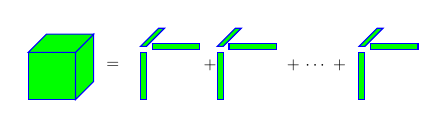
\begin{tikzpicture}[scale=0.15, every node/.style={transform shape}]
	\pgfmathsetmacro{\cubex}{4}
	\pgfmathsetmacro{\cubey}{4}
	\pgfmathsetmacro{\cubez}{4}
	\draw[blue,fill=pastelgreen] (0,0,0) -- ++(-\cubex,0,0) -- ++(0,-\cubey,0) -- ++(\cubex,0,0) -- cycle;
	\draw[blue,fill=pastelgreen] (0,0,0) -- ++(0,0,-\cubez) -- ++(0,-\cubey,0) -- ++(0,0,\cubez) -- cycle;
	\draw[blue,fill=pastelgreen] (0,0,0) -- ++(-\cubex,0,0) -- ++(0,0,-\cubez) -- ++(\cubex,0,0) -- cycle;
	
	\node[draw=none, text=black, scale=4] at (2,-2.25,-3) {$=$};
	\pgfmathsetmacro{\smallwidth}{0.5}
	\draw[blue,fill=pastelgreen] (\cubex+2,0,0) -- ++(-\smallwidth,0,0) -- ++(0,-\cubey,0) -- ++(\smallwidth,0,0) -- cycle;
	\draw[blue,fill=pastelgreen] (\cubex+2 +\cubex + 0.5,0.75,0) -- ++(-\cubex,0,0) -- ++(0,-\smallwidth,0) -- ++(\cubex,0,0) -- cycle;
	\draw[blue,fill=pastelgreen] (\cubex+2,0.5,0) -- ++(-\smallwidth,0,0) -- ++(0,0,-\cubez) -- ++(\smallwidth,0,0) -- cycle;
	
	\node[draw=none, text=black, scale=4] at (2+\cubex+4.25,-2.25,-3) {$+$};
	
	\draw[blue,fill=pastelgreen] (\cubex+2.5 + \cubex+2,0,0) -- ++(-\smallwidth,0,0) -- ++(0,-\cubey,0) -- ++(\smallwidth,0,0) -- cycle;
	\draw[blue,fill=pastelgreen] (\cubex+2.5+\cubex+2 +\cubex + 0.5,0.75,0) -- ++(-\cubex,0,0) -- ++(0,-\smallwidth,0) -- ++(\cubex,0,0) -- cycle;
	\draw[blue,fill=pastelgreen] (\cubex+2.5+\cubex+2,0.5,0) -- ++(-\smallwidth,0,0) -- ++(0,0,-\cubez) -- ++(\smallwidth,0,0) -- cycle;
	
	\node[draw=none, text=black, scale=4] at (2+\cubex+5 + \cubex+ 4.25, -2.25,-3) {$+$ $\cdots$ $+$};
	
	\draw[blue,fill=pastelgreen] (12 + \cubex+2.5 + \cubex+2,0,0) -- ++(-\smallwidth,0,0) -- ++(0,-\cubey,0) -- ++(\smallwidth,0,0) -- cycle;
	\draw[blue,fill=pastelgreen] (12+\cubex+2.5+\cubex+2 +\cubex + 0.5,0.75,0) -- ++(-\cubex,0,0) -- ++(0,-\smallwidth,0) -- ++(\cubex,0,0) -- cycle;
	\draw[blue,fill=pastelgreen] (12 + \cubex+2.5+\cubex+2,0.5,0) -- ++(-\smallwidth,0,0) -- ++(0,0,-\cubez) -- ++(\smallwidth,0,0) -- cycle;
	
	\end{tikzpicture}
\end{center}
	\end{minipage}
	\begin{minipage}{0.665\linewidth}
		\begin{itemize}
			\item No deterministic algorithm to find the decomposition
			\item Analyse one iteration of the popular existing algorithms
%%			\item Matricized tensor times Khatri-Rao product (MTTKRP)  is the most time consuming operation
%%			\begin{itemize}
%%				\item MTTKRP: ({$\mathcal{X}$}, \{$A_1, \cdots ,A_{k-1}, A_{k+1},\cdots,A_d$\}) $\longrightarrow$ $A_k$
%%			\end{itemize}
%%			\item Determine communication lower bounds for MTTKRP operation
			
			\item Propose and implement scalable algorithms for one iteration
		\end{itemize}	
	\end{minipage}
\end{block}\vspace*{-0.15cm}
\begin{block}{Tensor Train decomposition}
	\begin{minipage}{0.325\linewidth}
			\begin{center}
			\begin{tikzpicture}[scale=0.25, every node/.style={transform shape}]
			
			\node (t0) at (0,-2) [scale=4] {\tensor{A}};
			\node [scale=4]at (2, -2) {$=$};
			\path (5,-5) -- (0,0);
			\end{tikzpicture}\hspace*{-0.25cm}
			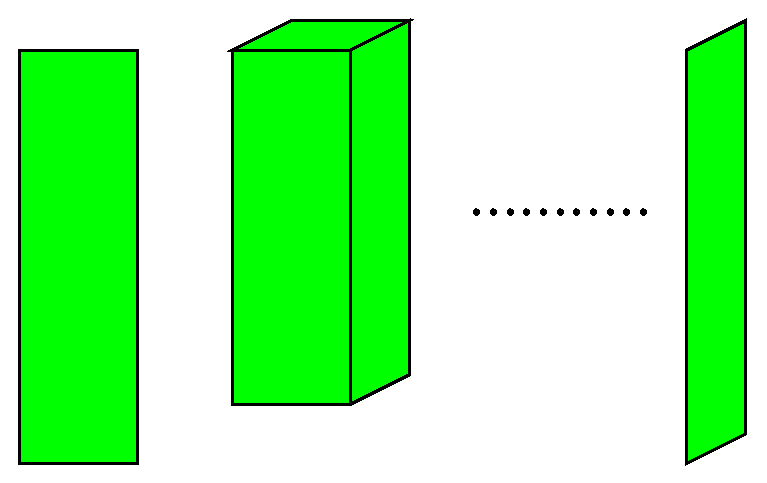
\includegraphics[scale=0.165]{./diagrams/ttentry-simple.eps}
		\end{center}
	\end{minipage}
	\begin{minipage}{0.665\linewidth}
		\begin{itemize}
			\item Determine communication lower bounds for this operation
			\vfill
			\item Analyse communication performed by popular algorithm
%%			: \textcolor{green}{Completed}
			\vfill
			\item Propose and implement new scalable communication algorithms
		\end{itemize}
	\end{minipage}
\end{block}
}
\end{frame}




\begin{frame}{Proving communication lower bounds for parallel computations}
\vspace*{-0.15cm}
{\footnotesize\begin{block}{How people did it for linear algebra operations?}
\begin{itemize}
	\item People obtain results for matrix multiplication operations
	\item Same lower bounds apply to almost all direct linear linear algebra operations using reduction [Ballard et. al., 09]
	, for instance, bound for LU factorization\vspace*{-0.15cm}
	{\scriptsize\begin{align*}
		\begin{pmatrix}
		I &  & -B\\
		A & I &  &\\
		& & I
		\end{pmatrix}
		&=
	\begin{pmatrix}
	I & &\\
	A & I & \\
	&& I
	\end{pmatrix}
	\begin{pmatrix}
	I & & -B \\
	& I & AB\\
	& & I
	\end{pmatrix}
	\end{align*}}
\end{itemize}
\end{block}

\vspace*{-0.15cm}{\footnotesize\begin{block}{Approach to compute lower bounds for tensor computations}
Notation: Tensors are denoted by solid shapes and number of lines denote the dimensions of the tensors. Connecting two lines implies summation (or contraction) over the connected dimensions. 	
	\begin{itemize}
		\item Obtain bounds for basic tensor operations: Tensor times matrix (TTM), Multiple tensor times matrix (Multi-TTM), Tensor contraction
		
		
%%		\includegraphics[scale=0.02]{./tmp/tensorBasicOperations.jpg}
\vspace*{-0.25cm}\begin{center}
%%	 \begin{tikzpicture}[scale=0.45, every node/.style={transform shape}]
%%	\tikzstyle{taskc}=[circle, draw=black, minimum size=3mm, fill=\tensorcolor]
%%	\node (t01) at (0,0) [taskc]{};
%%	\draw (t01) -- (0.75,0);
%%	\draw (t01) -- (-0.75,0);
%%	\draw (t01) -- (0,0.75);
%%	\node (t02) at (0,0.75) [taskc]{};
%%	
%%	\path (0,-0.75) -- (0,-0.75);
%%	\end{tikzpicture} $\qquad$
	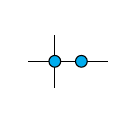
\begin{tikzpicture}[scale=0.45, every node/.style={transform shape}]
	\tikzstyle{taskc}=[circle, draw=black, minimum size=3mm, fill=\tensorcolor]
	\node (t01) at (0,0) [taskc]{};
	\draw (t01) -- (1.5,0);
	\draw (t01) -- (-0.75,0);
	\draw (t01) -- (0,0.75);
	\draw (t01) -- (0,-0.75);
	\node (t02) at (0.75,0) [taskc]{};
	
	\path (0, -0.95) -- (0, 0.95);
	
	\end{tikzpicture} $\qquad$
	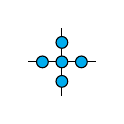
\begin{tikzpicture}[scale=0.45, every node/.style={transform shape}]
	\tikzstyle{taskc}=[circle, draw=black, minimum size=3mm, fill=\tensorcolor]

		
%%	\node (t01) at (0,-0.75) [taskc]{};
%%	\node (t02) at (0.56,-0.56) [taskc]{};
%%	\node (t03) at (0.56, 0.56) [taskc]{};
%%	\node (t04) at (0,0.75) [taskc]{};
%%	\node (t05) at (-0.56, 0.56) [taskc]{};
%%	\node (t06) at (-0.56, -0.56) [taskc]{};
%%	
%%	
%%	\draw (t01) -- (t04);
%%	\draw (t02) -- (t05);
%%	\draw (t03) -- (t06);

	\draw (-0.95, 0) -- (0.95, 0);
	\draw (0, -0.95) -- (0, 0.95);	

	\node (t01) at (0,-0.55) [taskc]{};
	\node (t02) at (0,0.55) [taskc]{};
	\node (t03) at (-0.55, 0) [taskc]{};
	\node (t04) at (0.55, 0) [taskc]{};
	

	\node (t00) at (0,0) [taskc]{};
	
	\path (0, -0.95) -- (0, 0.95);
						
%%	\draw (t01) -- (0.75,0);
%%	\draw (t01) -- (-0.75,0);
%%	\draw (t01) -- (0,0.75);
%%	\draw (t01) -- (0,-0.75);
%%	\node (t02) at (0.75,0) [taskc]{};
	\end{tikzpicture} $\qquad$
	\begin{tikzpicture}[scale=0.45, every node/.style={transform shape}]
	\tikzstyle{taskc}=[circle, draw=black, minimum size=3mm, fill=\tensorcolor]
	\node (t01) at (0,0) [taskc]{};
	\draw (t01) -- (0.75,0);
	\draw (t01) -- (-0.75,0);
	\draw (t01) -- (0,0.75);
	\draw (t01) -- (0,-0.75);
	\draw (t01) -- (-0.56, -0.56);
	
	\node (t02) at (0.75,0) [taskc]{};
	\draw (t02) -- (0.75,0.75);
	\draw (t02) -- (0.75,-0.75);
	
	\path (0, -0.95) -- (0, 0.95);
	\end{tikzpicture}
\end{center}
\vspace*{-0.25cm}				
	\item Express decompositions and manipulations in terms of these basis operations
\end{itemize}
\end{block}}
}\end{frame}


%%\subsection{Multi-TTM Computation}
%%\begin{frame}
%%\frametitle{Table of Contents}
%%\tableofcontents[currentsubsection]
%%\end{frame}


\begin{frame}{Communication lower bounds on $P$ processors}
\begin{itemize}
	\item Recently started to work with L. Grigori (Inria Paris, France), H. Daas (Rutherford Appleton Laboratory, UK)  and G. Ballard (Wake Forest University, USA)
	\vfill
	\item Revisited communication lower bounds for matrix multiplications
	\begin{minipage}{0.475\linewidth}
		\begin{itemize}
			\item Expressed existing approaches in suitable forms for tensors
			\item Lower bounds also instruct arrangement of processors in optimal algorithms 
			\item Improved the constants in the existing ranges of P (Demmel et.al [IPDPS 2013])
		\end{itemize}
	\end{minipage}$\quad$
	\begin{minipage}{0.45\linewidth}
		\begin{exampleblock}{Arrangements of $8$ processors}
\begin{center}
	\begin{tikzpicture}[scale=0.35, every node/.style={transform shape}]	
	\foreach \x in {0, 1, 2, 3, 4, 5, 6, 7, 8}
	\draw (-1, \x) -- (0, \x);
	
	\foreach \x in {0, 1, 2, 3, 4, 5, 6, 7, 8}
	\draw (0, \x)--(0.6, 0.5+\x);
	
	\draw (0,0) -- (0,8);
	\draw(-1,0)--(-1,8);
	\draw (0.6,0.5) -- (0.6,8.5);
	\draw (-1,8) -- (-1+0.6,8.5);
	
	\draw (-1+0.6,8.5) -- (0.6,8.5);
	
	\end{tikzpicture}$\qquad\quad$
	\begin{tikzpicture}[scale=0.35, every node/.style={transform shape}]
	
	\foreach \x in {0, 1, 2, 3, 4}
	\draw (-2, \x) -- (0, \x);
	
	\foreach \x in {0, 1, 2, 3, 4}
	\draw (0, \x)--(0.6, 0.5+\x);
	
	\draw (0,0) -- (0,4);
	\draw (-1,0) -- (-1,4);
	\draw(-2,0)--(-2,4);
	
	\draw (0.6,0.5) -- (0.6,4.5);
	
	\draw (-2,4) -- (-2+0.6, 4+0.5);
	\draw (-2+0.6, 4+0.5) -- (0.6, 4.5);
	
	\draw (-1,4) -- (-1+0.6, 4+0.5);
	
	%%\draw (-1,8) -- (0,8.5);
	%%\draw (0,8.5) -- (1,8.5);
	
	\end{tikzpicture}$\qquad\quad$
	\begin{tikzpicture}[scale=0.35, every node/.style={transform shape}]
	
	\def\xref{0.6}
	\def\yref{0.5}
	
	\foreach \x in {0, 1, 2}
	\draw (-2, \x) -- (0, \x);
	
	\foreach \x in {0, 1, 2}
	\draw (0, \x)--(2*\xref, 2*\yref+\x);
	
	\draw (0,0) -- (0,2);
	\draw (-1,0) -- (-1,2);
	\draw (-2,0)--(-2,2);
	\draw (\xref,\yref) -- (\xref, 2+\yref);
	\draw (2*\xref,2*\yref) -- (2*\xref, 2+ 2*\yref);
	
	\draw (-2,2) -- (-2+2*\xref, 2+2*\yref);
	\draw (-1,2) -- (-1+2*\xref, 2+2*\yref);
	
	\draw (-2+2*\xref, 2+2*\yref) -- (2*\xref, 2+2*\yref);
	\draw (-2+\xref, 2+\yref) -- (\xref, 2+\yref);
	\end{tikzpicture}
\end{center}
		\end{exampleblock}
	\end{minipage}
	\vfill
	\item Plan to continue this collaboration to compute lower bounds for tensor computations
 \end{itemize}
\end{frame}

%%%%\begin{frame}{Communication lower bound of 3-dimensional Multi-TTM computation}
%%%%%%\end{frame}
%%%%%%
%%%%%%\begin{frame}{Communication Optimal Algorithms for Tensors}
%%%%%%\begin{columns}
%%%%%%\begin{column}[c]{.25\textwidth}
%%%%%%%%		\includegraphics[width=\textwidth]{figs/sunway-taihulight.jpg}
%%%%%%\end{column}
%%%%%%\begin{column}[c]{.75\textwidth}
%%%%%%\includegraphics[scale=0.25]{./diagrams/ttentry}
%%%%%%\end{column}
%%%%%%\end{columns}
%%%%%%\begin{itemize}
%%%%%%\item This is a hard problem to start with
%%%%%%\item We look similar computation which has simpler structure than this
%%%%%%\end{itemize}
%%%%%%\begin{block}{3-dimensional Multiple Tensor Times Matrix (Multi TTM)}
%%%%\begin{center}
%%%%\begin{tikzpicture}[scale=0.15, every node/.style={transform shape}]
%%%%\pgfmathsetmacro{\cubex}{2}
%%%%\pgfmathsetmacro{\cubey}{2}
%%%%\pgfmathsetmacro{\cubez}{2}
%%%%\draw[blue,fill=pastelgreen] (-14,-1,\cubez-2) -- ++(-\cubex,0,0) -- ++(0,-\cubey,0) -- ++(\cubex,0,0) -- cycle;
%%%%\draw[blue,fill=pastelgreen] (-14,-1,\cubez-2) -- ++(0,0,-\cubez) -- ++(0,-\cubey,0) -- ++(0,0,\cubez) -- cycle;
%%%%\draw[blue,fill=pastelgreen] (-14,-1,\cubez-2) -- ++(-\cubex,0,0) -- ++(0,0,-\cubez) -- ++(\cubex,0,0) -- cycle;
%%%%\node[draw=none, text=black, scale=4] at (-11,-1,0) {$=$};
%%%%
%%%%\pgfmathsetmacro{\cubex}{4}
%%%%\pgfmathsetmacro{\cubey}{4}
%%%%\pgfmathsetmacro{\cubez}{4}
%%%%
%%%%\pgfmathsetmacro{\xs}{2}
%%%%\pgfmathsetmacro{\ys}{2}
%%%%\pgfmathsetmacro{\zs}{2}
%%%%
%%%%\draw[blue,fill=pastelgreen] (0,0,0) -- ++(-\cubex,0,0) -- ++(0,-\cubey,0) -- ++(\cubex,0,0) -- cycle;
%%%%\draw[blue,fill=pastelgreen] (0,0,0) -- ++(0,0,-\cubez) -- ++(0,-\cubey,0) -- ++(0,0,\cubez) -- cycle;
%%%%\draw[blue,fill=pastelgreen] (0,0,0) -- ++(-\cubex,0,0) -- ++(0,0,-\cubez) -- ++(\cubex,0,0) -- cycle;
%%%%
%%%%\draw[blue,fill=pastelgreen] (-\cubex-1,0,0) -- ++(-\cubex,0,0) -- ++(0,-\ys,0) -- ++(\cubex,0,0) -- cycle;
%%%%
%%%%\draw[blue,fill=pastelgreen] (\xs+1,0,-\cubey) -- ++(-\xs,0,0) -- ++(0,-\cubey,0) -- ++(\xs,0,0) -- cycle;
%%%%
%%%%\draw[blue,fill=pastelgreen] (0,0,-\cubez-1) -- ++(-\cubex,0,0) -- ++(0,0,-\zs-1) -- ++(\cubex,0,0) -- cycle;
%%%%\end{tikzpicture}
%%%%\end{center}
%%%%%%\end{block}
%%%%%%%%\end{frame}
%%%%%%%%
%%%%%%%%
%%%%%%%%%\begin{frame}
%%%%%%%%%\end{frame}
%%%%%%%%
%%%%%%%%\begin{frame}{Revisiting Matrix Multiplication Algorithms}
%%%%\begin{itemize}
%%%%\item It is an ongoing work
%%%%\item We revisited lower bounds for matrix multiplication
%%%%\item Our goal was to express existing approaches in the form suitable for tensors
%%%%\end{itemize}
%%%%
%%%%%%\begin{block}{Communication Optimal Matrix Multiplication Algorithm}
%%%%%%\includegraphics[scale=0.02]{./tmp/3d-mm.jpg}
%%%%%%\end{block}
%%%%%%\begin{itemize}
%%%%%%\item Reinvented many times: Dekel, Nassimi, Sahni [81], Bernsten [89], Agarwal, Chandra, Snir [90], Johnson [93], Agarwal, Balle, Gustavson, Joshi, Palkar [95]
%%%%%%\end{itemize}
%%%%\begin{block}{Different arrangements of 8 processors}
%%%%\begin{center}
%%%%\begin{tikzpicture}[scale=0.35, every node/.style={transform shape}]
%%%%%%\tikzstyle{taske}=[ellipse, draw=black, minimum width=25mm, minimum height=8mm, fill=\tensorcolor]
%%%%%%\node (t0) at (0,0) [taske] {};
%%%%%%
%%%%%%\foreach \x in {1, -0.75, -1}
%%%%%%\draw (\x, 1.25) -- (\x, 0);
%%%%%%
%%%%%%\draw [dotted] (-0.5, 0.7) -- (0.75, 0.7);
%%%%%%
%%%%%%%%	\foreach \y/\l in { 0/{0.4/0, 0.3/0.4, 0.7/0.7}, 
%%%%%%%%		0.5/{0.3/0, 0.4/0.3, 0.3/0.7},
%%%%%%%%		1.25/{0.5/0, 0.3/0.5, 1.2/0.8, 1.5/2.0},
%%%%%%%%		1.75/{0.8/0, 0.4/0.8, 0.7/1.2, 0.5/1.9},
%%%%%%%%		2.25/{0.6/0, 0.4/0.6, 1.1/1.0, 1.0/2.1},
%%%%%%%%	} {
%%%%%%%%		\foreach \w/\x in \l
%%%%%%%%		\node at (\x, \y)[task, minimum width=\w cm, fill=white] {};
%%%%%%%%	}
%%%%%%
%%%%%%
%%%%%%\node (t0) at (0,0) [taske] {\tensor{A}};
%%%%%%\node [scale=2]at (2, 0.0) {$=$};
%%%%%%\path (5,-6) -- (0,0);
%%%%
%%%%\foreach \x in {0, 1, 2, 3, 4, 5, 6, 7, 8}
%%%%\draw (-1, \x) -- (0, \x);
%%%%
%%%%\foreach \x in {0, 1, 2, 3, 4, 5, 6, 7, 8}
%%%%\draw (0, \x)--(0.6, 0.5+\x);
%%%%
%%%%\draw (0,0) -- (0,8);
%%%%\draw(-1,0)--(-1,8);
%%%%\draw (0.6,0.5) -- (0.6,8.5);
%%%%\draw (-1,8) -- (-1+0.6,8.5);
%%%%
%%%%\draw (-1+0.6,8.5) -- (0.6,8.5);
%%%%
%%%%\end{tikzpicture}$\qquad\quad$
%%%%\begin{tikzpicture}[scale=0.35, every node/.style={transform shape}]
%%%%%%\tikzstyle{taske}=[ellipse, draw=black, minimum width=25mm, minimum height=8mm, fill=\tensorcolor]
%%%%%%\node (t0) at (0,0) [taske] {};
%%%%%%
%%%%%%\foreach \x in {1, -0.75, -1}
%%%%%%\draw (\x, 1.25) -- (\x, 0);
%%%%%%
%%%%%%\draw [dotted] (-0.5, 0.7) -- (0.75, 0.7);
%%%%%%
%%%%%%%%	\foreach \y/\l in { 0/{0.4/0, 0.3/0.4, 0.7/0.7}, 
%%%%%%%%		0.5/{0.3/0, 0.4/0.3, 0.3/0.7},
%%%%%%%%		1.25/{0.5/0, 0.3/0.5, 1.2/0.8, 1.5/2.0},
%%%%%%%%		1.75/{0.8/0, 0.4/0.8, 0.7/1.2, 0.5/1.9},
%%%%%%%%		2.25/{0.6/0, 0.4/0.6, 1.1/1.0, 1.0/2.1},
%%%%%%%%	} {
%%%%%%%%		\foreach \w/\x in \l
%%%%%%%%		\node at (\x, \y)[task, minimum width=\w cm, fill=white] {};
%%%%%%%%	}
%%%%%%
%%%%%%
%%%%%%\node (t0) at (0,0) [taske] {\tensor{A}};
%%%%%%\node [scale=2]at (2, 0.0) {$=$};
%%%%%%\path (5,-6) -- (0,0);
%%%%
%%%%\foreach \x in {0, 1, 2, 3, 4}
%%%%\draw (-2, \x) -- (0, \x);
%%%%
%%%%\foreach \x in {0, 1, 2, 3, 4}
%%%%\draw (0, \x)--(0.6, 0.5+\x);
%%%%
%%%%\draw (0,0) -- (0,4);
%%%%\draw (-1,0) -- (-1,4);
%%%%\draw(-2,0)--(-2,4);
%%%%
%%%%\draw (0.6,0.5) -- (0.6,4.5);
%%%%
%%%%\draw (-2,4) -- (-2+0.6, 4+0.5);
%%%%\draw (-2+0.6, 4+0.5) -- (0.6, 4.5);
%%%%
%%%%\draw (-1,4) -- (-1+0.6, 4+0.5);
%%%%
%%%%%%\draw (-1,8) -- (0,8.5);
%%%%%%\draw (0,8.5) -- (1,8.5);
%%%%
%%%%\end{tikzpicture}$\qquad\quad$
%%%%\begin{tikzpicture}[scale=0.35, every node/.style={transform shape}]
%%%%%%\tikzstyle{taske}=[ellipse, draw=black, minimum width=25mm, minimum height=8mm, fill=\tensorcolor]
%%%%%%\node (t0) at (0,0) [taske] {};
%%%%%%
%%%%%%\foreach \x in {1, -0.75, -1}
%%%%%%\draw (\x, 1.25) -- (\x, 0);
%%%%%%
%%%%%%\draw [dotted] (-0.5, 0.7) -- (0.75, 0.7);
%%%%%%
%%%%%%%%	\foreach \y/\l in { 0/{0.4/0, 0.3/0.4, 0.7/0.7}, 
%%%%%%%%		0.5/{0.3/0, 0.4/0.3, 0.3/0.7},
%%%%%%%%		1.25/{0.5/0, 0.3/0.5, 1.2/0.8, 1.5/2.0},
%%%%%%%%		1.75/{0.8/0, 0.4/0.8, 0.7/1.2, 0.5/1.9},
%%%%%%%%		2.25/{0.6/0, 0.4/0.6, 1.1/1.0, 1.0/2.1},
%%%%%%%%	} {
%%%%%%%%		\foreach \w/\x in \l
%%%%%%%%		\node at (\x, \y)[task, minimum width=\w cm, fill=white] {};
%%%%%%%%	}
%%%%%%
%%%%%%
%%%%%%\node (t0) at (0,0) [taske] {\tensor{A}};
%%%%%%\node [scale=2]at (2, 0.0) {$=$};
%%%%%%\path (5,-6) -- (0,0);
%%%%
%%%%\def\xref{0.6}
%%%%\def\yref{0.5}
%%%%
%%%%\foreach \x in {0, 1, 2}
%%%%\draw (-2, \x) -- (0, \x);
%%%%
%%%%\foreach \x in {0, 1, 2}
%%%%\draw (0, \x)--(2*\xref, 2*\yref+\x);
%%%%
%%%%\draw (0,0) -- (0,2);
%%%%\draw (-1,0) -- (-1,2);
%%%%\draw (-2,0)--(-2,2);
%%%%\draw (\xref,\yref) -- (\xref, 2+\yref);
%%%%\draw (2*\xref,2*\yref) -- (2*\xref, 2+ 2*\yref);
%%%%
%%%%\draw (-2,2) -- (-2+2*\xref, 2+2*\yref);
%%%%\draw (-1,2) -- (-1+2*\xref, 2+2*\yref);
%%%%
%%%%\draw (-2+2*\xref, 2+2*\yref) -- (2*\xref, 2+2*\yref);
%%%%\draw (-2+\xref, 2+\yref) -- (\xref, 2+\yref);
%%%%
%%%%%%\draw (0.6,0.5) -- (0.6,4.5);
%%%%%%
%%%%%%\draw (-2,4) -- (-2+0.6, 4+0.5);
%%%%%%\draw (-2+0.6, 4+0.5) -- (0.6, 4.5);
%%%%%%
%%%%%%\draw (-1,4) -- (-1+0.6, 4+0.5);
%%%%
%%%%%%\draw (-1,8) -- (0,8.5);
%%%%%%\draw (0,8.5) -- (1,8.5);
%%%%\end{tikzpicture}
%%%%%%\begin{tikzpicture}
%%%%%%%%\draw [thick,fill=green] (0,0) to [out=90,in=150] (1,1) -- (.85,.15) -- (0,0);
%%%%%%\draw[thin] (-2, 0) -- node[above,scale=0.85]{$A(0,0)$} (-1, 0) -- (-1,1) -- (-2,1) -- (-2,0) ;
%%%%%%\end{tikzpicture}
%%%%\end{center}
%%%%\end{block}
%%%%\end{frame}
%%%%
%%%%\begin{frame}{Communication lower bounds for Matrix Multiplications on $P$ Processors}
%%%%
%%%%{\footnotesize
%%%%\begin{itemize}
%%%%	\item Each processor asymptotically performs the same amount of computation
%%%%	\item One copy of data is distributed among processor
%%%%\end{itemize}
%%%%\vspace*{-0.15cm}
%%%%\begin{block}{Square matrix multiplication}
%%%%	\begin{itemize}
%%%%		\item Communication optimal algorithms consider 3-dimensional processor arrangement
%%%%		\item Rediscovered many times in literature
%%%%	\end{itemize}
%%%%\end{block}
%%%%\vspace*{-0.15cm}
%%%%\begin{block}{Rectangular matrix multiplication $C=AB$}
%%%%Assume $n_1 \le n_2 \le n_3$ and dimensions of $A$, $B$, and $C$ are $n_1 \times n_2$, $n_2\times n_3$ and $n_1 \times n_3$.
%%%%	\begin{itemize}
%%%%		\item Lower bounds depend on the dimensions of the matrices
%%%%		\item Requires to solve a linear program
%%%%		\item Lower bounds also instruct the arrangement of processors in optimal algorithms 
%%%%%%		\item Processor arrangements depend on the dimensions of the matrices
%%%%		\begin{tikzpicture}
%%%%		\draw [|-] (0,0) -- node [above]{$1D-grid$} (4,0);
%%%%		\draw [|-](4,0) -- node [above] {$2D-grid$} (8,0);
%%%%		\draw [|->](8,0) -- node [above]{$3D-grid$}(12,0);
%%%%		
%%%%		\node at (0,0) [below, blue] {$1$};
%%%%		\node at (4,0) [below, blue] {$\frac{n_3}{n_2}$};
%%%%		\node at (8,0) [below, blue] {$\frac{n_2n_3}{n_1^2}$};
%%%%		
%%%%		\node at (12,0) [above, blue] {$P$};
%%%%		\end{tikzpicture}
%%%%		\vspace*{-0.25cm}
%%%%		\item  Improved the constants in the existing ranges of $P$ (Demmel et.al [IPDPS 2013]) 
%%%%	\end{itemize}
%%%%\end{block}
%%%%}
%%%%
%%%%\end{frame}
%%%%%%\begin{frame}{Processors Arranged in Different Ways}
%%%%%%Assume $n_1 \le n_2 \le n_3$ and dimensions of $A$, $B$, and $C$ are $n_2 \times n_1$, $n_1\times n_3$ and $n_2 \times n_3$ respectively.
%%%%%%\begin{block}{Three different arrangements of processor grids}
%%%%%%
%%%%%%\includegraphics[scale=0.02]{./tmp/processorRearrangement.jpg}
%%%%%%\end{block}
%%%%%%\end{frame}
%%%%%%\begin{frame}{Lower Bounds for Matrix Multiplication Algorithms}
%%%%%%
%%%%%%\includegraphics[scale=0.02]{./tmp/loomisWhitney.jpg}
%%%%%%From Loomis-Whitney inequality,
%%%%%%\begin{align*}
%%%%%%V_x V_y V_z \ge& V^2
%%%%%%\end{align*}
%%%%%%Atleast one processor will perform atleast $\frac{n_1n_2n_3}{P}$ computations. From Loomis-Whitney inequality, $\phi_A \phi_B \phi_C \ge \Big(\frac{n_1n_2n_3}{P}\Big)^2$.
%%%%%%
%%%%%%Here $\phi_A$, $\phi_B$ and $\phi_C$ denote the projections of computations on $A$, $B$ and $C$ matrices. Our goal is to minimize $\phi_A + \phi_B + \phi_C$.
%%%%%%
%%%%%%We also added other inequalities.
%%%%%%\begin{itemize}
%%%%%%\item To perform atleast $\frac{1}{P}$th computation, the processor must access atleast $\frac{1}{P}$th data of each matrix
%%%%%%\item Projectin on each matrix can not be larger than the original matrix
%%%%%%\end{itemize} 
%%%%%%We obtain the following additional inequalities.
%%%%%%\begin{align*}
%%%%%%\frac{n_1n_2}{P} \le \phi_A & \le n_1n_2\\
%%%%%%\frac{n_1n_3}{P} \le \phi_B & \le n_1n_3\\
%%%%%%\frac{n_2n_3}{P} \le \phi_C & \le n_2n_3
%%%%%%\end{align*}
%%%%%%
%%%%%%\end{frame}
%%%%
%%%%%%\begin{frame}{Lower Bounds for Matrix Multiplication Algorithms}
%%%%%%After solving the minimization problem we obtain the following ranges for different arrangement of process grids.
%%%%%%
%%%%%%\begin{itemize}
%%%%%%\item We corrected the constants in the existing ranges of $P$ (Demmel, Eliahu, Fox, Kamil, Lipshitz, Schwartz, Spillinger [IPDPS 2013])
%%%%%%\end{itemize}
%%%%%%\end{frame}
%%%%%%\begin{frame}{Multiple Tensor Times Matrix (Multi-TTM) Computations}
%%%%%%content...
%%%%%%\end{frame}
%%%%\begin{frame}{Lower Bounds for 3-dimensional Multi-TTM Computations}
%%%%Let \tensor{G} and \tensor{X} are output and input tensors. $A$, $B$ and $C$ are factor matrices, which are multiplied to the input tensor in 1st, 2nd and 3rd dimensions. Sizes of $\tensor{G}$, $\tensor{X}$, $A$, $B$, $C$ are $r_1\times r_2 \times r_3$, $n_1 \times n_2 \times n_3$, $n_1 \times r_1$, $n_2 \times r_2$ and $n_3 \times r_3$ respectively. Sequential code for this computation can be written as..
%%%%\begin{columns}
%%%%	\begin{column}{0.45\linewidth}
%%%%\begin{block}{}
%%%%\begin{center}
%%%%\begin{tikzpicture}[scale=0.25, every node/.style={transform shape}]
%%%%\pgfmathsetmacro{\cubex}{2}
%%%%\pgfmathsetmacro{\cubey}{2}
%%%%\pgfmathsetmacro{\cubez}{2}
%%%%\draw[blue,fill=pastelgreen] (-14,-1,\cubez-2) -- ++(-\cubex,0,0) -- ++(0,-\cubey,0) -- ++(\cubex,0,0) -- cycle;
%%%%\draw[blue,fill=pastelgreen] (-14,-1,\cubez-2) -- ++(0,0,-\cubez) -- ++(0,-\cubey,0) -- ++(0,0,\cubez) -- cycle;
%%%%\draw[blue,fill=pastelgreen] (-14,-1,\cubez-2) -- ++(-\cubex,0,0) -- ++(0,0,-\cubez) -- ++(\cubex,0,0) -- cycle;
%%%%\node[draw=none, text=black, scale=4] at (-11,-1,0) {$=$};
%%%%
%%%%\pgfmathsetmacro{\cubex}{4}
%%%%\pgfmathsetmacro{\cubey}{4}
%%%%\pgfmathsetmacro{\cubez}{4}
%%%%
%%%%\pgfmathsetmacro{\xs}{2}
%%%%\pgfmathsetmacro{\ys}{2}
%%%%\pgfmathsetmacro{\zs}{2}
%%%%
%%%%\draw[blue,fill=pastelgreen] (0,0,0) -- ++(-\cubex,0,0) -- ++(0,-\cubey,0) -- ++(\cubex,0,0) -- cycle;
%%%%\draw[blue,fill=pastelgreen] (0,0,0) -- ++(0,0,-\cubez) -- ++(0,-\cubey,0) -- ++(0,0,\cubez) -- cycle;
%%%%\draw[blue,fill=pastelgreen] (0,0,0) -- ++(-\cubex,0,0) -- ++(0,0,-\cubez) -- ++(\cubex,0,0) -- cycle;
%%%%
%%%%\draw[blue,fill=pastelgreen] (-\cubex-1,0,0) -- ++(-\cubex,0,0) -- ++(0,-\ys,0) -- ++(\cubex,0,0) -- cycle;
%%%%
%%%%\draw[blue,fill=pastelgreen] (\xs+1,0,-\cubey) -- ++(-\xs,0,0) -- ++(0,-\cubey,0) -- ++(\xs,0,0) -- cycle;
%%%%
%%%%\draw[blue,fill=pastelgreen] (0,0,-\cubez-1) -- ++(-\cubex,0,0) -- ++(0,0,-\zs-1) -- ++(\cubex,0,0) -- cycle;
%%%%\end{tikzpicture}
%%%%\end{center}
%%%%\end{block}
%%%%\end{column}\hfill
%%%%{\tiny\begin{column}{0.5\linewidth}
%%%%\begin{algorithmic}
%%%%	\FOR{$i_1=1:n_1$}
%%%%	\FOR{$i_2=1:n_2$}
%%%%	\FOR{$i_3=1:n_3$}
%%%%	\FOR{$j_1=1:r_1$}
%%%%	\FOR{$j_2=1:r_2$} 
%%%%	\FOR{$j_3=1:r_3$} 
%%%%	\STATE {$\tensor{G}(j_1,j_2, j_3) += \tensor{X}(i_1,i_2,i_3)*A(i_1,j_1)*B(i_2,j_2)*B(i_3,j_3)$} 
%%%%	\ENDFOR 	
%%%%	\ENDFOR 	
%%%%	\ENDFOR 
%%%%	\ENDFOR
%%%%	\ENDFOR
%%%%	\ENDFOR
%%%%\end{algorithmic}
%%%%\end{column}}
%%%%\end{columns}
%%%%
%%%%\end{frame}

%%\begin{frame}{3-dimensional Multi TTM Computation}
%%\begin{algorithmic}
%%\FOR{$i_1=1:n_1$}
%%\FOR{$i_2=1:n_2$}
%%\FOR{$i_3=1:n_3$}
%%\FOR{$j_1=1:r_1$}
%%\FOR{$j_2=1:r_2$} 
%%\FOR{$j_3=1:r_3$} 
%%\STATE {$\tensor{G}(j_1,j_2, j_3) += \tensor{X}(i_1,i_2,i_3)*A(i_1,j_1)*B(i_2,j_2)*B(i_3,j_3)$} 
%%\ENDFOR 	
%%\ENDFOR 	
%%\ENDFOR 
%%\ENDFOR
%%\ENDFOR
%%\ENDFOR
%%\end{algorithmic}
%%\end{frame}

%%\begin{frame}{Lower communication bounds for 3-dimensional Multi-TTM}
%%\begin{itemize}
%%	\item We apply similar approach for this computation
%%	\item Lower bounds suggest to consider the following arrangements of processors for the optimal algorithms
%%	\begin{center}
%%	\begin{tabular}{|c|c|}
%%		\hline
%%		Processor Range & Type of Arrangement\\ \hline
%%		$P < \min\Big(\frac{n_3r_3}{n_2r_2}, \frac{n_1n_2n_3}{r_1r_2r_3}\Big)$ & 1D-grid \\ \hline
%%		$ \frac{n_1n_2n_3}{r_1r_2r_3} < P \le \frac{n_3r_3}{n_2r_2}$ & 2D-grid\\ \hline
%%		$\frac{n_3r_3}{n_2r_2} \le P < \min\Big(\frac{n_1n_2n_3}{r_1r_2r_3}, \frac{n_2n_3r_2r_3}{n_1^2r_1^2}\Big)$ & 2D-grid\\ \hline
%%		$\max\Big(\frac{n_3r_3}{n_2r_2}, \frac{n_1n_2n_3}{r_1r_2r_3}\Big) \le P < \frac{n_2n_3r_2r_3}{n_1^2r_1^2}$ & 4D-grid\\ \hline
%%		$\frac{n_2n_3r_2r_3}{n_1^2r_1^2} \le P < \frac{n_1n_2n_3}{r_1r_2r_3}$ & 3D-grid\\ \hline
%%		$\max\Big(\frac{n_2n_3r_2r_3}{n_1^2r_1^2}, \frac{n_1n_2n_3}{r_1r_2r_3}\Big) \le P$ & 6D-grid\\ \hline
%%	\end{tabular}
%%	\end{center}
%%\end{itemize}
%%\end{frame}
%%\begin{frame}{Multi TTM Computation}
%%$\phi_x$ denotes the projection of iteration space on variable $x$. Here $x\in {G, \mathcal{X}, A, B, C}$. Dimension of $\tensor{G}$, $\mathcal{X}$, $A$, $B$, $C$ are $r_1\times r_2 \times r_3$, $n_1 \times n_2 \times n_3$, $n_1 \times r_1$, $n_2 \times r_2$ and $n_3 \times r_3$ respectively. We assume $r_1r_2r_3 \le n_1n_2n_3$ and $n_1r_1 \le n_2r_2 \le n_3r_3$.
%%
%%We need to solve the following linear program:
%%
%%Minimize $\phi_G + \phi_X + \phi_A +\phi_A +\phi_B + \phi_C$ subject to
%%\begin{align*}
%%\phi_G \phi_X \ge & \frac{n_1n_2n_3r_1r_2r_3}{P}\\
%%\phi_A \phi_B \phi_C \ge & \frac{n_1n_2n_3r_1r_2r_3}{P}\\
%%\frac{n_1n_2n_3}{P} \le \phi_X \le& n_1n_2n_3\\
%%\frac{r_1r_2r_3}{P} \le \phi_G \le& r_1r_2r_3\\
%%\frac{n_1r_1}{P} \le \phi_A \le& n_1r_1\\
%%\frac{n_2r_2}{P} \le \phi_B \le& n_2r_2\\
%%\frac{n_3r_3}{P} \le \phi_C \le& n_3r_3
%%\end{align*}
%%
%%After solving this linear program, we obtain  different communication lower bounds based on the number of processors ($P$) used.
%%\end{frame}
%%
%%
%%\begin{frame}{Multi TTM Computation}
%%\includegraphics[scale=0.02]{./tmp/processorRangeMultiTMM.jpg}
%%Lower bound on the communication for the processor $\ge $ $\phi_G + \phi_X + \phi_A +\phi_A +\phi_B + \phi_C$ - \textit{Portion of the variables already present in the memory}
%%\end{frame}

%%\begin{frame}{Modify Existing Algorithms}
%%\begin{itemize}
%%	\item Understand the existing Algorithms
%%	\item Derive communication lower bounds 
%%	\item Design new algorithms \& implement them
%%	\item Homogeneous Systems
%%	\item Extend the same principle for Heterogeneous Systems
%%\end{itemize}
%%\end{frame}
%%\setcounter{section}{20}
\section{Extension of Existing Approaches/Algorithms (Short/Mid Term Research Plans)}
\begin{frame}
\frametitle{Research Project}
\tableofcontents[currentsection]
\end{frame}
%%\subsubsection{Tensor Contraction and Strassen's Matrix Multiplication}
%%\begin{frame}{Tensor Contraction \& Strassen's Matrix Multiplication}
%%content...
%%\end{frame}


\begin{frame}{Strassen's concepts to tensors}
\vspace*{-0.175cm}
{\footnotesize
\begin{block}{Matrix multiplication of $n\times n$ square matrices }
	\begin{itemize}
		\item Complexity of traditional matrix multiplication is $\mathcal{O}(n^3)$ 
		\item Strassen's matrix multiplication
		\begin{itemize}
			\item Expressed matrix multiplication as a tensor computation
			\item Canonical rank of the tensor determines the complexity of the computation
			\item Complexity is $\mathcal{O}(n^{2.81})$
		\end{itemize}
	\item Plan to extend Strassen's concepts to tensor contractions
	\end{itemize}
\end{block}}\vspace*{-0.15cm}
\begin{exampleblock}{Contraction of a 3-dimensional tensor with a matrix}{\scriptsize
		\begin{minipage}{0.5\linewidth}\vspace*{-0.05cm}
\begin{algorithmic}
	\FOR{$i_1=1:n$}
	\FOR{$i_2=1:n$}
	\FOR{$i_3=1:n$}
	\FOR{$j_2=1:n$} 
	\STATE {$\tensor{G}(i_1,i_2,j_2) = \tensor{G}(i_1,i_2,j_2) + \tensor{A}(i_1,i_2,i_3)*B(i_3,j_2)$} 
	\ENDFOR
	\ENDFOR
	\ENDFOR
	\ENDFOR
\end{algorithmic}
		\end{minipage}
	\begin{minipage}{0.45\linewidth}{\footnotesize
		\begin{itemize}
			\item Total $\mathcal{O}(n^{4})$ operations
			\item Apply Strassen's algorithm for each $i_1$, total $\mathcal{O}(n^{3.81})$ operations 
			\item Expressing as a canonical decomposition of $8\times8\times4$ tensor can further reduces the number of operations
		\end{itemize}
	}\end{minipage}
}\end{exampleblock}
\end{frame}

%%\begin{frame}{$2\times2$ recursive Matrix Multiplication $C=AB$}
%%$\textcolor{blue}{\bullet}$ Matrix is divided into 2$\times$2 blocks
%%\vspace*{-0.1cm}
%%\begin{center}{\footnotesize
%%$\begin{pmatrix}
%%	C_{11} & C_{12} \\
%%	C_{21} & C_{22}
%%\end{pmatrix}
%%$
%%=$
%%\begin{pmatrix}
%%	A_{11} & A_{12} \\
%%	A_{21} & A_{22}
%%\end{pmatrix}
%%\begin{pmatrix}
%%	B_{11} & B_{12} \\
%%	B_{21} & B_{22}
%%\end{pmatrix}$
%%%%
%%%%\vspace*{-0.25cm}
%%%%		\begin{align*}
%%%%\begin{pmatrix}
%%%%C_{11} & C_{12} \\
%%%%C_{21} & C_{22}
%%%%\end{pmatrix}
%%%%&
%%%%=
%%%%\begin{pmatrix}
%%%%A_{11} & A_{12} \\
%%%%A_{21} & A_{22}
%%%%\end{pmatrix}
%%%%\begin{pmatrix}
%%%%B_{11} & B_{12} \\
%%%%B_{21} & B_{22}
%%%%\end{pmatrix}
%%%%\end{align*}
%%}\end{center}
%%\vspace*{-0.25cm}
%%\begin{columns}{\footnotesize
%%
%%	\begin{column}{0.375\linewidth}
%%		\begin{block}{Traditional Algorithm}		
%%			\begin{align*}
%%			C_{11} &= A_{11}B_{11} + A_{12}B_{21}\\
%%			C_{12} &= A_{11}B_{12} + A_{12}B_{22}\\
%%			C_{21} &= A_{21}B_{11} + A_{22}B_{21}\\
%%			C_{22} &= A_{21}B_{12} + A_{22}B_{22}\\
%%			\end{align*}
%%		\end{block}
%%	Operation count recurrence,
%%	
%%	$\qquad T(n) = 8T\Big(\frac{n}{2}\Big) + \mathcal{O}(n^2)$, $T(n) = 1$\\
%%%%	\begin{align*}
%%%%	T(n) &= 8T\Big(\frac{n}{2}\Big) + \mathcal{O}(n^2)\\T(n) &= 1
%%%%	\end{align*}	
%%	After solving, we obtain $T(n) = \mathcal{O}(n^3)$
%%	\end{column}
%%\hfill\begin{column}{0.6\linewidth}
%%		\begin{block}{Strassen's Algorithm}
%%%%		\begin{align*}
%%%%		\begin{pmatrix}
%%%%		C_{11} & C_{12} \\
%%%%		C_{21} & C_{22}
%%%%		\end{pmatrix}
%%%%		&
%%%%		=
%%%%		\begin{pmatrix}
%%%%		A_{11} & A_{12} \\
%%%%		A_{21} & A_{22}
%%%%		\end{pmatrix}
%%%%		\begin{pmatrix}
%%%%		B_{11} & B_{12} \\
%%%%		B_{21} & B_{22}
%%%%		\end{pmatrix}
%%%%		\end{align*}
%%\begin{minipage}{0.56\linewidth}
%%	\vspace*{-0.5cm}
%%		\begin{align*}
%%M_1 &= (A_{11} + A_{22})(B_{11}+B_{22})\\
%%M_2 &= (A_{21} + A_{22})B_{11}\\
%%M_3 &= A_{11} (B_{12}-B_{22})\\
%%M_4 &= A_{22} (B_{21}-B_{11})\\
%%M_5 &= (A_{11} +A_{12})B_{22}\\
%%M_6 &= (A_{21}-A_{11})(B_{11} +B_{12})\\
%%M_7 &= (A_{12}-A_{22})(B_{21} + B_{22}) 
%%\end{align*}
%%\end{minipage}
%%\begin{minipage}{0.425\linewidth}
%%		\begin{align*}
%%C_{11} &= M_1 + M_4 -M_5 +M_7\\
%%C_{12} &= M_3 + M_5\\
%%C_{21} &= M_2 + M_4\\
%%C_{22} &= M_1 -M_2 + M_3 + M_6
%%\end{align*}
%%\end{minipage}
%%	\end{block}
%%%%\vspace*{-0.25cm}
%%	Operation count recurrence, $ T(n) = 7T\Big(\frac{n}{2}\Big) + \mathcal{O}(n^2)$, $T(n) = 1$\\
%%%%	\begin{align*}
%%%%	T(n) &= 8T\Big(\frac{n}{2}\Big) + \mathcal{O}(n^2)\\T(n) &= 1
%%%%	\end{align*}	
%%After solving, we obtain $T(n) = \mathcal{O}(n^{2.81})$
%%	\end{column}
%%}\end{columns}
%%\end{frame}
%%
%%\begin{frame}{$2\times 2$ Matrix multiplication as a tensor operation}
%%%%\begin{itemize}
%%%%%%	\item C = AB
%%%%	\item Matrix is divided into 2$\times$2 blocks
%%%%\end{itemize}
%%\vspace*{-0.15cm}
%%\begin{center}{
%%		$\begin{pmatrix}
%%		C_{11} & C_{12} \\
%%		C_{21} & C_{22}
%%		\end{pmatrix}
%%		$
%%		=$
%%		\begin{pmatrix}
%%		A_{11} & A_{12} \\
%%		A_{21} & A_{22}
%%		\end{pmatrix}
%%		\begin{pmatrix}
%%		B_{11} & B_{12} \\
%%		B_{21} & B_{22}
%%		\end{pmatrix}$
%%}\end{center}
%%\vspace*{-0.15cm}We can write this multiplication as a tensor operation,
%%\begin{align*}
%%\tensor{T}\times_1 \begin{pmatrix}
%%A_{11}\\
%%A_{12}\\
%%A_{21}\\
%%A_{22}
%%\end{pmatrix}
%%\times_2 \begin{pmatrix}
%%B_{11}\\
%%B_{12}\\
%%B_{21}\\
%%B_{22}
%%\end{pmatrix}
%%&=\begin{pmatrix}
%%C_{11}\\
%%C_{12}\\
%%C_{21}\\
%%C_{22}
%%\end{pmatrix}
%%\end{align*}
%%	Where \tensor{T} is a $4\times4\times4$ tensor with the following slices:
%%	\begin{align*}\tiny
%%	T_1= \begin{pmatrix}
%%	1&0&0&0\\
%%	0&0&1&0\\
%%	0&0&0&0\\
%%	0&0&0&0
%%	\end{pmatrix}
%%	&\tiny
%%	T_2= \begin{pmatrix}
%%	0&1&0&0\\
%%	0&0&0&1\\
%%	0&0&0&0\\
%%	0&0&0&0
%%	\end{pmatrix}
%%	&\tiny
%%	T_3= \begin{pmatrix}
%%	0&0&0&0\\
%%	0&0&0&0\\
%%	1&0&0&0\\
%%	0&0&1&0
%%	\end{pmatrix}
%%	&\tiny
%%	T_4= \begin{pmatrix}
%%	0&0&0&0\\
%%	0&0&0&0\\
%%	0&1&0&0\\
%%	0&0&0&1
%%	\end{pmatrix}
%%	\end{align*}
%%	\textcolor{blue}{$\bullet$} Canonical rank of \tensor{T} = $7$, which determines the complexity of Strassen's algorithm
%%\end{frame}
%%
%%
%%\begin{frame}{Tensor contractions}
%%$\tensor{A}$ $\in$ $\mathbb{R}^{n_1 \times n_2 \times \cdots \times n_{d_1}}$, $\tensor{B}$ $\in$ $\mathbb{R}^{m_1 \times m_2 \times \cdots \times m_{d_2}}$ and we want to compute $\tensor{A}\times_{n_i}\tensor{B}$ where $n_i=m_j$.
%%
%%%%For $d_1=3$, $d_2=2$, $n_1=n_2=n_3=m_1=m_2=n$, $i=3$, and $j=1$. We assume that the output tensor is $\tensor{G}$ and its all elements are initialized to zero. We can compute $\tensor{G}$ with the following algorithm:
%%\begin{itemize}
%%	\item $d_1=3$, $d_2=2$, $n_1=n_2=n_3=m_1=m_2=n$, $i=3$, and $j=1$
%%	\item Output tensor is $\tensor{G}$ and its all elements are initialized to zero
%%\end{itemize}
%%%%\end{frame}
%%%%\begin{frame}{Tensor contractions}
%%\begin{algorithmic}
%%	\FOR{$i_1=1:n$}
%%	\FOR{$i_2=1:n$}
%%	\FOR{$i_3=1:n$}
%%	\FOR{$j_2=1:n$} 
%%	\STATE {$\tensor{G}(i_1,i_2,j_2) = \tensor{G}(i_1,i_2,j_2) + \tensor{A}(i_1,i_2,i_3)*\tensor{B}(i_3,j_2)$} 
%%	\ENDFOR
%%	\ENDFOR
%%	\ENDFOR
%%	\ENDFOR
%%\end{algorithmic}
%%\begin{itemize}
%%	\item Total $\mathcal{O}(n^{4})$ operations
%%	\item Applying Strassen's algorithm for each $i_1$, total $\mathcal{O}(n^{3.81})$ operations 
%%\end{itemize}
%%\end{frame}
%%
%%\begin{frame}{Tensor contractions with Strassen's concept}
%%\begin{itemize}
%%\item Expressing this computation as canonical low rank decomposition of $8\times8\times4$ tensor can further reduce the number of operations
%%\end{itemize}
%%\begin{align*}
%%\tensor{T}\times_1 \begin{pmatrix}
%%\tensor{A}_{111}\\
%%\tensor{A}_{112}\\
%%\tensor{A}_{121}\\
%%\tensor{A}_{122}\\
%%\tensor{A}_{211}\\
%%\tensor{A}_{212}\\
%%\tensor{A}_{221}\\
%%\tensor{A}_{222}
%%\end{pmatrix}
%%\times_2 \begin{pmatrix}
%%B_{11}\\
%%B_{12}\\
%%B_{21}\\
%%B_{22}
%%\end{pmatrix}
%%&=\begin{pmatrix}
%%\tensor{G}_{111}\\
%%\tensor{G}_{112}\\
%%\tensor{G}_{121}\\
%%\tensor{G}_{122}\\
%%\tensor{G}_{211}\\
%%\tensor{G}_{212}\\
%%\tensor{G}_{221}\\
%%\tensor{G}_{222}
%%\end{pmatrix}
%%\end{align*}
%%\end{frame}

%%\subsection{Hierarchical Matrix concepts to Tensors}
\begin{frame}{Hierarchical Matrix concepts to Tensors}
\begin{block}{Hierarchical Matrices}
\begin{itemize}
	\item Data sparse approximation of non-sparse matrices
\begin{center}

\begin{tikzpicture}[scale=0.425, every node/.style={transform shape}]

\tikzstyle{taskr}=[draw=black, minimum height=32mm, minimum width=32mm, fill=none, text=black]

\node (t0) at (0,0) [taskr] {};
\node [below,scale=1.5] at (t0.south) {Original Matrix};

\end{tikzpicture}$\qquad\qquad$
\begin{tikzpicture}[scale=0.425, every node/.style={transform shape}]

\tikzstyle{taskr}=[draw=black, minimum height=32mm, minimum width=32mm, fill=none, text=black]

\node (t0) at (0,0) [taskr] {};
\node [below,scale=1.5] at (t0.south) {Step 1};

\node (t00) at (0,0) [taskr, anchor=north east, minimum width=16mm, minimum height=16mm] {LR};
\node (t00) at (0,0) [taskr, anchor=south west, minimum width=16mm, minimum height=16mm] {LR};

\end{tikzpicture}$\qquad\qquad$
\begin{tikzpicture}[scale=0.425, every node/.style={transform shape}]

\tikzstyle{taskr}=[draw=black, minimum height=32mm, minimum width=32mm, fill=none, text=black]

\node (t0) at (0,0) [taskr] {};
\node [below,scale=1.5] at (t0.south) {Step 2};

\node (t00) at (0,0) [taskr, anchor=north east, minimum width=16mm, minimum height=16mm] {LR};
\node (t00) at (0,0) [taskr, anchor=south west, minimum width=16mm, minimum height=16mm] {LR};



\node (t000) at (t0.west) [taskr, anchor=south west, minimum width=8mm, minimum height=8mm] {LR};
\node (t001) at (t000.north east) [taskr, anchor=south west, minimum width=8mm, minimum height=8mm] {LR};

\node (t000) at (t0.south) [taskr, anchor=south west, minimum width=8mm, minimum height=8mm] {LR};
\node (t001) at (t000.north east) [taskr, anchor=south west, minimum width=8mm, minimum height=8mm] {LR};
\end{tikzpicture}
\end{center}
\end{itemize}
\noindent $LR$: low rank block
\end{block}

\begin{block}{Tensors}
	\begin{minipage}{0.565\linewidth}
	\begin{itemize}
		\item $f(i,j,k) = \frac{1}{|i-j|+|j-k|+|k-i|}$
		\item Value is small if difference of any pair is large
		\item Formalize and evaluate this approach for tensors
	\end{itemize}
	\end{minipage}
\begin{minipage}{0.4\linewidth}
			\begin{center}
		\begin{tikzpicture}[scale=0.5, every node/.style={transform shape}]
		
		\def\xref{0.6}
		\def\yref{0.5}
		
		\draw (0,0) -- (2,0)--(2,2)--(0,2)--(0,0);
		\draw (2,0) -- (2+2*\xref, 2*\yref) -- (2+2*\xref, 2+2*\yref) -- (2,2) -- (2,0);
		\draw (0,2) -- (2,2) -- (2+2*\xref, 2+2*\yref) -- (2*\xref, 2+2*\yref) --(0,2);
		\node [below] at (1,0) {Original Tensor};
		\end{tikzpicture}$\qquad\qquad$
		\begin{tikzpicture}[scale=0.5, every node/.style={transform shape}]
		%%\draw[thin] (-2, 0) -- node[above,scale=0.85]{$A(0,0)$} (-1, 0) -- (-1,1) -- (-2,1) -- (-2,0) ;
		\draw (0,0) -- node [above] {LR}(1,0) -- (1,1) -- (0,1)--(0,0);
		\draw (1,0) -- node [above] {LR}(2,0) -- (2,1) -- (1,1)--(1,0);
		\draw [fill=green] (0,1) -- (1,1) -- (1,2) -- (0,2)--(0,1);
		\draw  (1,1) -- node [above] {LR}(2,1) -- (2,2) -- (1,2)--(1,1);
		
		\def\xref{0.6}
		\def\yref{0.5}
		
		\draw (2,0) -- (2+\xref, \yref) -- (2+\xref, \yref +1) -- (2,1) -- (2,0);
		\draw (2,1) -- (2+\xref, 1+\yref) -- (2+\xref, 2+\yref ) -- (2,2) -- (2,1);
		
		\draw [fill=green](2+\xref,0+\yref) -- (2+2*\xref, 2*\yref) -- (2+2*\xref, 2*\yref +1) -- (2+\xref,1+\yref) -- (2+\xref,\yref);
		\draw (2+\xref,1+\yref) -- node [above] {LR}(2+2*\xref, 1+2*\yref) -- (2+2*\xref, 2*\yref +2) -- (2+\xref,2+\yref) -- (2+\xref,1+\yref);
		
		
		\draw [fill=green] (0,2) --  (1,2) -- (1+\xref, 2+\yref) -- (\xref, 2+\yref) -- (0,2);
		\draw (1,2) -- (2,2) -- (2+\xref, 2+\yref) -- (1+\xref, 2+\yref) -- (1,2);
		\draw (0+\xref,2+\yref) -- node [sloped, above right,rotate=0] {LR} (1+\xref,2+\yref) -- (1+2*\xref, 2+2*\yref) -- (2*\xref, 2+2*\yref) -- (0+\xref,2+\yref);
		\draw (1+\xref,2+\yref) --  (2+\xref,2+\yref) -- (2+2*\xref, 2+2*\yref) -- (1+2*\xref, 2+2*\yref) -- (1+\xref,2+\yref);
		
		\node [below] at (1,0) {Step 1};
		
		\end{tikzpicture}
	\end{center}
\end{minipage}
\end{block}
\end{frame}


%%\begin{frame}{Roofline model with Dependencies}
%%%%\begin{columns}
%%%%	\begin{column}{0.45\linewidth}
%%%%	\end{column}
%%%%\end{columns}
%%\vspace*{-0.35cm}
%%\begin{center}
%%\begin{minipage}{0.425\linewidth}
%%	\begin{block}{Iterative bound}
%%\centering \includegraphics[scale=0.285]{boundsDiagram/taskgraphOnePath}
%%	\end{block}
%%\end{minipage}$\qquad$
%%\begin{minipage}{0.425\linewidth}
%%	\begin{block}{Roofline Model}
%%			\includegraphics[scale=0.14]{./diagrams/Example_of_a_Roofline_model.png}
%%	\end{block}
%%\end{minipage}
%%\end{center}
%%%\begin{columns}
%%%	\begin{column}[c]{.5\linewidth}
%%%		\begin{block}{\centering {\scriptsize DAG}}
%%%			\only<1-3> {\centering \includegraphics[scale=0.25]{boundsDiagram/taskgraph}}
%%%			%\only<2-3> {\centering \includegraphics[scale=0.25]{boundsDiagram/taskgraphPath}}
%%%		\end{block}
%%%	\end{column}
%%	
%%%%	\begin{column}[c]{.5\linewidth}
%%%%		\begin{block}{\centering {\scriptsize \only<1> {No} \only<2-3> {Some} 
%%%%					Dependencies}}
%%%%			\only<1> {\centering \includegraphics[scale=0.25]{boundsDiagram/taskgraphNoDep}}
%%%%			\only<2-3> {\centering \includegraphics[scale=0.25]{boundsDiagram/taskgraphOnePath}}
%%%%		\end{block}
%%%%	\end{column}
%%%%\end{columns}
%%\begin{block}{\centering {\scriptsize Minimum execution time (minimize \textit{l})}}
%%	\begin{columns}
%%		\begin{column}[c]{.5\linewidth}
%%			\centering \includegraphics[scale=0.45]{boundsDiagram/schedule}   
%%		\end{column}
%%		\begin{column}[c]{.5\linewidth}
%%			\begin{itemize}
%%					\item[$\star$]{\scriptsize If any path in DAG is larger than \textit{l}}
%%						\begin{itemize}
%%							\item {\scriptsize add this path with data transfer cost as a constraint and repeat the procedure}
%%						\end{itemize}
%%				\end{itemize}			
%%		\end{column}  
%%	\end{columns}
%%\end{block}
%%\vspace*{-0.25cm}
%%\begin{itemize}
%%	\item Take minimum of both values as the lower bound of the application
%%\end{itemize}
%%\end{frame}

%%\subsection{Exploratory Topics}
\section{Exploratory Topics (Mid/Long Term Research Plans)}
\begin{frame}
\frametitle{Research Project}
\tableofcontents[currentsection]
\end{frame}

\begin{frame}{Tensor Representations for High Dimensional Tensors}
\begin{itemize}
	\item Tensor Train is a popular representation to work with high dimensional tensors
	\item Adding tensors and aplying an operator in this representation
	\begin{minipage}{0.475\linewidth}
	\begin{center}
			\begin{tikzpicture}[scale=0.35, every node/.style={transform shape}]
		\tikzstyle{taskc}=[circle, draw=black, minimum size=5mm, fill=\tensorcolor]
		%%	\node (t01) at (0,0) [taskc]{};
			
		\draw (2,0) -- (-2,0);
		
		\foreach \x in {1, 0.5, 0, -0.5, -1}
		\draw (2*\x, 0) -- (2*\x,0.75);
		
		\foreach \x in {1, 0.5, 0, -0.5, -1}
		\node at (2*\x, 0) [taskc] {};
		
		\node [below,scale=1.5] at (0,-1) {rank=$r$};
		
		\node [scale=2] at (3.25, 0) {$+\ $};
		
		\path (0, 1.45) -- (0, -1.45);
		\end{tikzpicture}
		\begin{tikzpicture}[scale=0.35, every node/.style={transform shape}]
		\tikzstyle{taskc}=[circle, draw=black, minimum size=5mm, fill=\tensorcolor]
		%%	\node (t01) at (0,0) [taskc]{};
		
		\draw (2,0) -- (-2,0);
		
		\foreach \x in {1, 0.5, 0, -0.5, -1}
		\draw (2*\x, 0) -- (2*\x,0.75);
		
		\foreach \x in {1, 0.5, 0, -0.5, -1}
		\node at (2*\x, 0) [taskc] {};
		
		\node [below,scale=1.5] at (0,-1) {rank=$s$};
		
		\node [scale=2] at (3.25, 0) {$=\ $};
		\path (0, 1.45) -- (0, -1.45);
		\end{tikzpicture}
		\begin{tikzpicture}[scale=0.35, every node/.style={transform shape}]
		\tikzstyle{taskc}=[circle, draw=black, minimum size=5mm, fill=\tensorcolor]
		%%	\node (t01) at (0,0) [taskc]{};
		
		\draw (2,0) -- (-2,0);
		
		\foreach \x in {1, 0.5, 0, -0.5, -1}
		\draw (2*\x, 0) -- (2*\x,0.75);
		
		\foreach \x in {1, 0.5, 0, -0.5, -1}
		\node at (2*\x, 0) [taskc] {};
		
		\node [below,scale=1.5] at (0,-1) {rank=$r+s$};
		\path (0, 1.45) -- (0, -1.45);
		\end{tikzpicture}
	\end{center}
	\end{minipage}$\quad$
\begin{minipage}{0.475\linewidth}
%%	\item Applying an operator in this representation
	\begin{center}
	\begin{tikzpicture}[scale=0.35, every node/.style={transform shape}]
	\tikzstyle{taskc}=[circle, draw=black, minimum size=5mm, fill=\tensorcolor]
	%%	\node (t01) at (0,0) [taskc]{};
	
	\draw (2,0) -- (-2,0);
	
	\foreach \x in {1, 0.5, 0, -0.5, -1}
	\draw (2*\x, 0) -- (2*\x,0.75);
	
	\foreach \x in {1, 0.5, 0, -0.5, -1}
	\node at (2*\x, 0) [taskc] {};
	
	\node [below,scale=1.5] at (0,-1) {rank=$r$};
	
	\node [scale=2] at (3.25, 0) {$\ $};
	\path (0, 1.45) -- (0, -1.45);
	\end{tikzpicture}
	\begin{tikzpicture}[scale=0.35, every node/.style={transform shape}]
	\tikzstyle{taskc}=[circle, draw=black, minimum size=5mm, fill=\tensorcolor]
	%%	\node (t01) at (0,0) [taskc]{};
	
	\draw (2,0) -- (-2,0);
	
	\foreach \x in {1, 0.5, 0, -0.5, -1}
	\draw (2*\x, 0) -- (2*\x,0.75);
	
	\foreach \x in {1, 0.5, 0, -0.5, -1}
	\draw (2*\x, 0) -- (2*\x,-0.75);
	
	\foreach \x in {1, 0.5, 0, -0.5, -1}
	\node at (2*\x, 0) [taskc] {};
	
	\node [below,scale=1.5] at (0,-1) {rank=$s$};
	
	\node [scale=2] at (3.25, 0) {$=\ $};
	\path (0, 1.45) -- (0, -1.45);
	\end{tikzpicture}
	\begin{tikzpicture}[scale=0.35, every node/.style={transform shape}]
	\tikzstyle{taskc}=[circle, draw=black, minimum size=5mm, fill=\tensorcolor]
	%%	\node (t01) at (0,0) [taskc]{};
	
	\draw (2,0) -- (-2,0);
	
	\foreach \x in {1, 0.5, 0, -0.5, -1}
	\draw (2*\x, 0) -- (2*\x,0.75);
	
	\foreach \x in {1, 0.5, 0, -0.5, -1}
	\node at (2*\x, 0) [taskc] {};
	
	\node [below,scale=1.5] at (0,-1) {rank=$r*s$};
	\path (0, 1.45) -- (0, -1.45);
	\end{tikzpicture}
\end{center}
\end{minipage}

	\item Requires a truncation  process which iterates over cores one by one 
	\item This representation is not much suited to work in parallel 
\end{itemize}

\begin{block}{New Tensor Representations}
\begin{itemize}
	\item Look at new representations in tree format -- suitable for parallelization
	%%	\vfill
	\begin{center}
		\begin{tikzpicture}[scale=0.35, every node/.style={transform shape}]
		\tikzstyle{taskc}=[circle, draw=black, minimum size=5mm, fill=\tensorcolor]
		
		\node (t) at (0,0) [taskc]{};
		\node (t0) at (-1,-1) [taskc]{};
		\node (t00) at (-2,-2) [taskc]{};
		\node (t01) at (-0.5,-2) [taskc]{};
		\node (t000) at (-3,-3) [taskc]{};
		\node (t001) at (-1.8,-3) [taskc]{};
		\node (t010) at (-1,-3) [taskc]{};
		\node (t011) at (-0.285,-3) [taskc]{};
		
		\draw (t) -- (t0);
		\draw (t0) -- (t00);
		\draw (t0) -- (t01);
		\draw (t00) -- (t000);
		\draw (t00) -- (t001);
		\draw (t01) -- (t010);
		\draw (t01) -- (t011);
		
		
		\node (t1) at (1,-1) [taskc]{};
		\node (t10) at (0.5,-2) [taskc]{};
		\node (t11) at (2,-2) [taskc]{};
		\node (t100) at (0.285,-3) [taskc]{};
		\node (t101) at (1,-3) [taskc]{};
		\node (t110) at (1.8,-3) [taskc]{};
		\node (t111) at (3,-3) [taskc]{};
		
		\draw (t) -- (t1);
		\draw (t1) -- (t10);
		\draw (t1) -- (t11);
		\draw (t10) -- (t100);
		\draw (t10) -- (t101);
		\draw (t11) -- (t110);
		\draw (t11) -- (t111);
		
		\node [scale=2] at (4.5,-2) {or};
		\end{tikzpicture} $\qquad$
		\begin{tikzpicture}[scale=0.35, every node/.style={transform shape}]
		\tikzstyle{taskc}=[circle, draw=black, minimum size=5mm, fill=\tensorcolor]
		
		\node (t) at (0,0) [taskc]{};
		\node (t0) at (-1,-1) [taskc]{};
		\node (t00) at (-2,-2) [taskc]{};
		\node (t01) at (-0.5,-2) [taskc]{};
		\node (t000) at (-3,-3) [taskc]{};
		\node (t001) at (-1.8,-3) [taskc]{};
		\node (t010) at (-1,-3) [taskc]{};
		\node (t011) at (-0.285,-3) [taskc]{};
		
		\draw (t) -- (t0);
		\draw (t0) -- (t00);
		\draw (t0) -- (t01);
		\draw (t00) -- (t000);
		\draw (t00) -- (t001);
		\draw (t01) -- (t010);
		\draw (t01) -- (t011);
		
		
		\node (t1) at (1,-1) [taskc]{};
		\node (t10) at (0.5,-2) [taskc]{};
		\node (t11) at (2,-2) [taskc]{};
		\node (t100) at (0.285,-3) [taskc]{};
		\node (t101) at (1,-3) [taskc]{};
		\node (t110) at (1.8,-3) [taskc]{};
		\node (t111) at (3,-3) [taskc]{};
		
		\draw (t) -- (t1);
		\draw (t1) -- (t10);
		\draw (t1) -- (t11);
		\draw (t10) -- (t100);
		\draw (t10) -- (t101);
		\draw (t11) -- (t110);
		\draw (t11) -- (t111);
		
		%%		\draw [thick,green] (t0) -- (t1);
		%%		\draw [thick,green] (t00) -- (t01);
		%%		\draw [thick,green] (t000) -- (t001);
		%%		\draw [thick,green] (t010) -- (t011);
		%%		\draw [thick,green] (t10) -- (t11);
		%%		\draw [thick,green] (t100) -- (t101);
		%%		\draw [thick,green] (t110) -- (t111);
		
		\draw [thick,green] (t01) -- (t10);
		\end{tikzpicture} 
		%%			\includegraphics[scale=0.02]{./tmp/newTensorRepresenattion.jpg}
	\end{center}
	\begin{itemize}
		\item Data will be stored at the leaf nodes
		\item Interal nodes will help to manipulate tensors in parallel
	\end{itemize}
%%	\vfill
%%	\item Some tensor representations exhibit tree structure
%%	\begin{itemize}
%%		\item Mainly designed to reduce storage or model long range interactions
%%		\item Not suitable to work with them in parallel
%%	\end{itemize}
\end{itemize}
\end{block}
\end{frame}


%%%%\begin{frame}{Architecture Aware Algorithms}
%%%%\begin{center}
%%%%	\begin{minipage}{0.45\columnwidth}
%%%%			\includegraphics[scale=0.25]{./diagrams/VoltaTensorCore.png}
%%%%	\end{minipage}
%%%%	\begin{minipage}{0.45\columnwidth}
%%%%		\includegraphics[scale=0.25]{./diagrams/A100_TensorCore_FP64.jpg}
%%%%	\end{minipage}
%%%%\end{center}
%%%%\begin{itemize}
%%%%	\item Recent Nvidia GPUs have tensor cores to accelerate AI computations
%%%%	\item Most linear algebra computations do not take advantages of these units
%%%%	\item Design algorithms which take architecture details into account
%%%%\end{itemize}
%%%%Fig source: \url{www.nvidia.com}
%%%%\end{frame}


\begin{frame}{Randomization in Tensor Computations}
\begin{itemize}
	\item Randomized SVD and UTV factorization are now well established
	\vfill
	\item Apply randomization to tensors
	\vfill
	\item Perform factorizations of tensors
	\begin{itemize}
		\item For example: QR like factorization of a tensor
	\end{itemize}
	\begin{center}
	\begin{tikzpicture}[scale=0.5, every node/.style={transform shape}]
	\tikzstyle{taske}=[ellipse, draw=black, minimum width=25mm, minimum height=8mm, fill=\tensorcolor]
	\node (t0) at (0,0) [taske] {};
	
	\foreach \x in {1, 0.75, 0.5, 0.25, 0, -0.25, -0.5, -0.75, -1}
	\draw (\x, 0.75) -- (\x, 0);
	
	%%	\foreach \y/\l in { 0/{0.4/0, 0.3/0.4, 0.7/0.7}, 
	%%		0.5/{0.3/0, 0.4/0.3, 0.3/0.7},
	%%		1.25/{0.5/0, 0.3/0.5, 1.2/0.8, 1.5/2.0},
	%%		1.75/{0.8/0, 0.4/0.8, 0.7/1.2, 0.5/1.9},
	%%		2.25/{0.6/0, 0.4/0.6, 1.1/1.0, 1.0/2.1},
	%%	} {
	%%		\foreach \w/\x in \l
	%%		\node at (\x, \y)[task, minimum width=\w cm, fill=white] {};
	%%	}
	
	
	\node (t0) at (0,0) [taske] {};
	\end{tikzpicture}$\qquad$
	\begin{tikzpicture}[scale=0.5, every node/.style={transform shape}]
	\tikzstyle{taskc}=[circle, draw=black, minimum size=5mm, fill=\tensorcolor]
	%%	\node (t01) at (0,0) [taskc]{};
	
	
	
	\draw (4,0) -- (-4,0);
	
	\foreach \x in {1, 0.75, 0.5, 0.25, 0, -0.25, -0.5, -0.75, -1}
	\draw (4*\x, 0) -- (4*\x,0.75);
	
	\foreach \x in {1, 0.75, 0.5, 0.25, 0, -0.25, -0.5, -0.75, -1}
	\node at (4*\x, 0) [taskc] {};
	
	\end{tikzpicture}
\end{center}
\end{itemize}
\end{frame}
%%\section{Integration in the Team}
%%%%%%%%\begin{frame}{Integration in the team}
%%%%%%%%%%\vspace*{-0.175cm}
%%%%%%%%
%%%%%%%%{\footnotesize
%%%%%%%%
%%%%%%%%%%\vspace*{-0.1cm}
%%%%%%%%\begin{tikzpicture}[scale=0.625, every node/.style={transform shape}]
%%%%%%%%\tikzstyle{taskr}=[draw=black, rounded corners, minimum height=30mm, minimum width=70mm, fill=none, text=black]
%%%%%%%%
%%%%%%%%
%%%%%%%%%%\tikzstyle{taskcompute}=[draw=black, minimum height=16mm, minimum width=16mm, fill=none, text=black, below]
%%%%%%%%
%%%%%%%%
%%%%%%%%\node (mainfocus) at (0,0) [taskr, anchor=south] {};
%%%%%%%%\node at (mainfocus.south) [below] {\textbf{Main focus}};
%%%%%%%%
%%%%%%%%\node [below, align=left, text width=70mm]at (mainfocus.north) {		\textbf{$\ $Scalable communication optimal algorithms for tensors}\\{\footnotesize \mybullet Analyze existing algorithms\\ 
%%%%%%%%		\mybullet Determine communication lower bounds\\\mybullet Propose communication optimal algorithms\\\mybullet Implement the proposed algorithms}};
%%%%%%%%
%%%%%%%%
%%%%%%%%\node (shorttermfocus) at (8,0) [taskr, minimum height=15mm, anchor=south] {};
%%%%%%%%\node at (shorttermfocus.south) [below] {\textbf{Short/Mid term plans}};
%%%%%%%%
%%%%%%%%\node [below, align=left, text width=70mm]at (shorttermfocus.north) {\footnotesize \mybullet Extend Strassen's concepts to tensors\\\mybullet Extend hierarchical matrices to tensors\\\mybullet Separation order of dimensions in tensor train};
%%%%%%%%
%%%%%%%%
%%%%%%%%\node (midtermfocus) at (16,0) [taskr, minimum height=20mm, anchor=south] {};
%%%%%%%%\node at (midtermfocus.south) [below] {\textbf{Mid/Long term plans}};
%%%%%%%%
%%%%%%%%\node [below, align=left, text width=70mm]at (midtermfocus.north) {\footnotesize \mybullet New tensor representations\\ \mybullet Architecture aware algorithms\\ \mybullet Randomization in tensors\\ \mybullet Factorizations of tensors};
%%%%%%%%
%%%%%%%%
%%%%%%%%
%%%%%%%%\tikzstyle{taske}=[ellipse, draw=black, minimum width=25mm, minimum height=8mm, fill=none]
%%%%%%%%
%%%%%%%%\node (bora) at (-1,5) [taske] {\textbf{Bora Ucar}};
%%%%%%%%\node [above, align=left, text width=35mm]at (bora.north) {Expert in sparse tensor computations};
%%%%%%%%
%%%%%%%%%%\draw [->] (bora) -- (mainfocus);
%%%%%%%%%%\draw [->] (bora) -- (shorttermfocus);
%%%%%%%%%%\draw [->] (bora) -- (midtermfocus);
%%%%%%%%
%%%%%%%%
%%%%%%%%\node (loris) at (4,5) [taske] {\textbf{$\ $Loris Marchal$\ $}};
%%%%%%%%\node [above, align=left, text width=42mm]at (loris.north) {Expert in communication and memory aware algorithms};
%%%%%%%%
%%%%%%%%%%\draw [->] (loris) -- (mainfocus);
%%%%%%%%%%\draw [->] (loris) -- (shorttermfocus);
%%%%%%%%%%\draw [->] (loris) -- (midtermfocus);
%%%%%%%%
%%%%%%%%
%%%%%%%%\node (others) at (11.8, 5) [taske, text width=40mm] {\textbf{Anne Benoit, Yves Robert and Frederic Vivien}};
%%%%%%%%\node [above, align=left, text width=60mm]at (others.north) {Expert in parallel algorithms and scheduling strategies};
%%%%%%%%
%%%%%%%%%%\draw [->] (others) -- (mainfocus);
%%%%%%%%%%\draw [->] (others) -- (shorttermfocus);
%%%%%%%%%%\draw [->] (others) -- (midtermfocus);
%%%%%%%%
%%%%%%%%
%%%%%%%%\node (gregoire) at (18, 5) [taske] {\textbf{Gregoire Pichon}};
%%%%%%%%\node [above, align=left, text width=40mm]at (gregoire.north) {Expert in low rank compression algorithms};
%%%%%%%%
%%%%%%%%%%\draw [->] (gregoire) -- (mainfocus);
%%%%%%%%%%\draw [->] (gregoire) -- (shorttermfocus);
%%%%%%%%%%\draw [->] (gregoire) -- (midtermfocus);
%%%%%%%%
%%%%%%%%\end{tikzpicture}
%%%%%%%%
%%%%%%%%\begin{block}{Bringing additional skills in the team}
%%%%%%%%	\begin{itemize}
%%%%%%%%		\item High dimensional dense tensor computations
%%%%%%%%		\item Communication lower bounds for linear algebra computations
%%%%%%%%		\item Scalable approaches for large HPC systems
%%%%%%%%		\item Use of tensors in quantum and molecular simulations 
%%%%%%%%		%%		\item Designing strategies to work with high dimensional tensor computations
%%%%%%%%		%%		\item Determining communication lower bounds for linear algebra computations
%%%%%%%%		%%		\item Designing scalable approaches for large HPC systems
%%%%%%%%		%%		\item Familiar with molecular and quantum simulations and how tensors are used in these domains 
%%%%%%%%	\end{itemize}
%%%%%%%%\end{block}
%%%%%%%%
%%%%%%%%}
%%%%%%%%\end{frame}


\begin{frame}{Integration in the ROMA team}
%%\vspace*{-0.175cm}

{\footnotesize
	
	%%\vspace*{-0.1cm}
	\begin{tikzpicture}[scale=0.625, every node/.style={transform shape}]
	\tikzstyle{taskr}=[draw=black, rounded corners, minimum height=30mm, minimum width=70mm, fill=none, text=black]
	
	
	%%\tikzstyle{taskcompute}=[draw=black, minimum height=16mm, minimum width=16mm, fill=none, text=black, below]
	
	
	\node (mainfocus) at (0,0) [taskr, anchor=south] {};
	\node at (mainfocus.south) [below] {\textbf{Main focus}};
	
	\node [below, align=left, text width=70mm]at (mainfocus.north) {		\textbf{$\ $Scalable communication optimal algorithms for tensors}\\{\footnotesize \mybullet Analyze existing algorithms\\ 
			\mybullet Determine communication lower bounds\\\mybullet Propose communication optimal algorithms\\\mybullet Implement the proposed algorithms}};
	
	
	\node (shorttermfocus) at (8,0) [taskr, minimum height=21mm, anchor=south] {};
	\node at (shorttermfocus.south) [below] {\textbf{Short/Mid term plans}};
	
	\node [below, align=left, text width=70mm]at (shorttermfocus.north) {\textbf{$\ $Extension of existing approaches\medskip}\\\footnotesize \mybullet Strassen's concepts to tensors\\\mybullet Concepts of hierarchical matrices to tensors\\\mybullet Separation order of dimensions in tensor train};
	
	
	\node (midtermfocus) at (16,0) [taskr, minimum height=25mm, anchor=south] {};
	\node at (midtermfocus.south) [below] {\textbf{Mid/Long term plans}};
	
	\node [below, align=left, text width=70mm]at (midtermfocus.north) {\textbf{$\ $Exploratory topics\medskip}\\\footnotesize \mybullet New tensor representations\\ \mybullet Architecture aware algorithms\\ \mybullet Randomization in tensors\\ \mybullet Factorizations of tensors};
	
	
	
	\tikzstyle{taske}=[ellipse, draw=black, minimum width=65mm, minimum height=30mm, fill=none]
	
	\node (expertise) at (10,4.75) [taske] {};
	\node at (expertise.south) [below] {\textbf{Expertise of the team}};
	\node [text width=56mm] at (expertise.mid) {\footnotesize \mybullet Parallel algorithms\\
	\mybullet Scheduling strategies\\
	\mybullet Memory aware algorithms\\
	\mybullet Sparse tensor computations\\
	\mybullet Low rank compression algorithms};


	\tikzstyle{taskt}=[ellipse, draw=black, minimum width=87.5mm, minimum height=15mm, fill=none]
	\node (team) at (1,5) [taskt] {};
	\node at (team.south) [below] {\textbf{Team}};
	\node [text width=70mm] at (team.mid) {Anne Benoit,
		Loris Marchal, 
		Gregoire Pichon,\\
		Yves Robert,
		Bora Ucar, and
		Frederic Vivien
		};



%%	\node (bora) at (-1,5) [taske] {\textbf{Bora Ucar}};
%%	\node [above, align=left, text width=35mm]at (bora.north) {Expert in sparse tensor computations};
%%	
%%	%%\draw [->] (bora) -- (mainfocus);
%%	%%\draw [->] (bora) -- (shorttermfocus);
%%	%%\draw [->] (bora) -- (midtermfocus);
%%	
%%	
%%	\node (loris) at (4,5) [taske] {\textbf{$\ $Loris Marchal$\ $}};
%%	\node [above, align=left, text width=42mm]at (loris.north) {Expert in communication and memory aware algorithms};
%%	
%%	%%\draw [->] (loris) -- (mainfocus);
%%	%%\draw [->] (loris) -- (shorttermfocus);
%%	%%\draw [->] (loris) -- (midtermfocus);
%%	
%%	
%%	\node (others) at (11.8, 5) [taske, text width=40mm] {\textbf{Anne Benoit, Yves Robert and Frederic Vivien}};
%%	\node [above, align=left, text width=60mm]at (others.north) {Expert in parallel algorithms and scheduling strategies};
%%	
%%	%%\draw [->] (others) -- (mainfocus);
%%	%%\draw [->] (others) -- (shorttermfocus);
%%	%%\draw [->] (others) -- (midtermfocus);
%%	
%%	
%%	\node (gregoire) at (18, 5) [taske] {\textbf{Gregoire Pichon}};
%%	\node [above, align=left, text width=40mm]at (gregoire.north) {Expert in low rank compression algorithms};
%%	
%%	%%\draw [->] (gregoire) -- (mainfocus);
%%	%%\draw [->] (gregoire) -- (shorttermfocus);
%%	%%\draw [->] (gregoire) -- (midtermfocus);
	
	\end{tikzpicture}
	
	\begin{block}{Bringing additional skills in the team}
		\begin{itemize}
			\item High dimensional dense tensor computations
			\item Communication lower bounds for linear algebra computations
			\item Scalable approaches for large HPC systems
			\item Use of tensors in quantum and molecular simulations 
			%%		\item Designing strategies to work with high dimensional tensor computations
			%%		\item Determining communication lower bounds for linear algebra computations
			%%		\item Designing scalable approaches for large HPC systems
			%%		\item Familiar with molecular and quantum simulations and how tensors are used in these domains 
		\end{itemize}
	\end{block}
	
	
	%%\begin{itemize}
	%%	\item Design and implementation of scalable tensor algorithms (\textbf{Bora Ucar})
	%%%%	Expert in sparse tensor computations. Work with him on the design and implementation of scalable algorithms 
	%%	\item Memory aware algorithms for tensors (\textbf{Loris Marchal})
	%%%%	Expert in the design of memory and communication oriented algorithms. Work with him on extending the roofline model with dependencies and memory aware algorithms to schedule tasks on HPC platforms
	%%	\item Parallel algorithms and scheduling strategies for tasks of tensor operations on homogeneous/heterogeneous systems (\textbf{Anne Benoit}, \textbf{Yves Robert} and \textbf{Frederic Vivien})
	%%%%	Experts in designing parallel algorithms and scheduling strategies. Work with them on the design of scalable parallel algorithms and scheduling strategies for homogeneous/heterogeneous systems
	%%	\item Extension of hierarchical matrices to tensors (\textbf{Gregoire Pichon})
	%%%%	 Works on low rank compression of matrices. Work with him on extending the concept of hierarchical matrices to tensors
	%%\end{itemize}
}
\end{frame}


%%%%
%%%%\begin{frame}{Test2}
%%%%\begin{tikzpicture}[scale=0.625, every node/.style={transform shape}]
%%%%\tikzstyle{taskr}=[draw=black, rounded corners, minimum height=30mm, minimum width=70mm, fill=none, text=black]
%%%%
%%%%
%%%%%%\tikzstyle{taskcompute}=[draw=black, minimum height=16mm, minimum width=16mm, fill=none, text=black, below]
%%%%
%%%%
%%%%\node (mainfocus) at (0,0) [taskr, anchor=south] {};
%%%%\node at (mainfocus.south) [below] {\textbf{Main Focus}};
%%%%
%%%%\node [below, align=left, text width=70mm]at (mainfocus.north) {		\textbf{$\ $Scalable communication optimal algorithms for tensors}\\{\footnotesize \mybullet Analyze existing algorithms\\ 
%%%%		\mybullet Determine communication lower bounds\\\mybullet Propose communication optimal algorithms\\\mybullet Implement the proposed algorithms}};
%%%%
%%%%
%%%%\node (shorttermfocus) at (8,0) [taskr, minimum height=15mm, anchor=south] {};
%%%%\node at (shorttermfocus.south) [below] {\textbf{Short term plans}};
%%%%
%%%%\node [below, align=left, text width=70mm]at (shorttermfocus.north) {\footnotesize \mybullet Extend Strassen's concepts to tensors\\\mybullet Extend hierarchical matrices to tensors\\\mybullet Separation order of dimensions in tensor train};
%%%%
%%%%
%%%%\node (midtermfocus) at (16,0) [taskr, minimum height=20mm, anchor=south] {};
%%%%\node at (midtermfocus.south) [below] {\textbf{Mid term plans}};
%%%%
%%%%\node [below, align=left, text width=70mm]at (midtermfocus.north) {\footnotesize \mybullet New tensor representations\\ \mybullet Architecture aware algorithms\\ \mybullet Randomization in tensors\\ \mybullet Factorizations of tensors};
%%%%
%%%%
%%%%
%%%%\tikzstyle{taske}=[ellipse, draw=black, minimum width=25mm, minimum height=8mm, fill=none]
%%%%
%%%%\node (bora) at (-1,6) [taske] {\textbf{Bora Ucar}};
%%%%\node [above, align=left, text width=40mm]at (bora.north) {Expert in sparse tensor computations};
%%%%
%%%%\draw [->] (bora) -- (mainfocus);
%%%%\draw [->] (bora) -- (shorttermfocus);
%%%%\draw [->] (bora) -- (midtermfocus);
%%%%
%%%%
%%%%\node (loris) at (4,6) [taske] {\textbf{Loris Marchal}};
%%%%\node [above, align=left, text width=40mm]at (loris.north) {Expert in communication and memory aware algorithms};
%%%%
%%%%\draw [->] (loris) -- (mainfocus);
%%%%\draw [->] (loris) -- (shorttermfocus);
%%%%\draw [->] (loris) -- (midtermfocus);
%%%%
%%%%
%%%%\node (others) at (12, 6) [taske, text width=50mm] {\textbf{Anne Benoit, Yves Robert and Frederic Vivien}};
%%%%\node [above, align=left, text width=70mm]at (others.north) {Expert in parallel algorithms and scheduling strategies};
%%%%
%%%%\draw [->] (others) -- (mainfocus);
%%%%\draw [->] (others) -- (shorttermfocus);
%%%%\draw [->] (others) -- (midtermfocus);
%%%%
%%%%
%%%%\node (gregoire) at (18, 6) [taske] {\textbf{Gregoire Pichon}};
%%%%\node [above, align=left, text width=40mm]at (gregoire.north) {Expert in low rank compression algorithms};
%%%%
%%%%\draw [->] (gregoire) -- (mainfocus);
%%%%\draw [->] (gregoire) -- (shorttermfocus);
%%%%\draw [->] (gregoire) -- (midtermfocus);
%%%%
%%%%\end{tikzpicture}
%%%%\end{frame}






%%\begin{frame}{Integration in the Team}
%%%%\vspace*{-0.25cm}
%%
%%{\footnotesize
%%	\begin{itemize}
%%		\item  \textbf{Bora Ucar}: Expert in sparse tensor computations. Work with him on the design and implementation of scalable algorithms 
%%		\item \textbf{Loris Marchal}: Expert in the design of memory and communication oriented algorithms. Work with him on extending the roofline model with dependencies and memory aware algorithms to schedule tasks on HPC platforms
%%		\item \textbf{Anne Benoit}, \textbf{Yves Robert} and \textbf{Frederic Vivien}: Experts in designing parallel algorithms and scheduling strategies. Work with them on the design of scalable parallel algorithms and scheduling strategies for homogeneous/heterogeneous systems
%%		\item \textbf{Gregoire Pichon}: Works on low rank compression of matrices. Work with him on extending the concept of hierarchical matrices to tensors
%%	\end{itemize}
%%	\begin{block}{Bringing additional skills in the team}
%%		\begin{itemize}
%%			\item Designing strategies to work with high dimensional tensor computations
%%			\item Determining communication lower bounds for linear algebra computations
%%			\item Designing scalable approaches for large HPC systems
%%			\item Familiar with molecular and quantum simulations and how tensors are used in these domains 
%%		\end{itemize}
%%	\end{block}
%%}
%%In my opinion, the ROMA team is the perfect team for my research project. Bora Ucar is an expert in tensor computations.
%%I would like to work with him on the design of novel compression and manipulation algorithms for high dimensional tensors.
%%Loris Marchal is an expert in the design of memory and communication oriented algorithms. I want to take his help in
%%extending roofline model with application characteristics. Anne Benoit, Yves Robert and Frederic Vivien are experts in
%%designing parallel algorithms and scheduling strategies for the modern computing systems. I intend to collaborate with
%%them on scalability and scheduling aspects of my project. Grégoire Pichon works on low rank compression of matrices.
%%I also intend to work with him on the design of low rank based scalable tensor compression algorithms. My profile fits
%%perfectly into the team and my experience with high dimensional tensors, and molecular and quantum simulations would
%%bring additional new skills in the team.
%%\end{frame}

%%%%%----------------------------------------------------------------------------------------
%%%%%	PRESENTATION SLIDES
%%%%%----------------------------------------------------------------------------------------
%%%%
%%%%%------------------------------------------------
%%%%\section{First Section} % Sections can be created in order to organize your presentation into discrete blocks, all sections and subsections are automatically printed in the table of contents as an overview of the talk
%%%%%------------------------------------------------
%%%%
%%%%\subsection{Subsection Example} % A subsection can be created just before a set of slides with a common theme to further break down your presentation into chunks
%%
%%\begin{frame}
%%\frametitle{Paragraphs of Text}
%%Sed iaculis dapibus gravida. Morbi sed tortor erat, nec interdum arcu. Sed id lorem lectus. Quisque viverra augue id sem ornare non aliquam nibh tristique. Aenean in ligula nisl. Nulla sed tellus ipsum. Donec vestibulum ligula non lorem vulputate fermentum accumsan neque mollis.\\~\\
%%
%%Sed diam enim, sagittis nec condimentum sit amet, ullamcorper sit amet libero. Aliquam vel dui orci, a porta odio. Nullam id suscipit ipsum. Aenean lobortis commodo sem, ut commodo leo gravida vitae. Pellentesque vehicula ante iaculis arcu pretium rutrum eget sit amet purus. Integer ornare nulla quis neque ultrices lobortis. Vestibulum ultrices tincidunt libero, quis commodo erat ullamcorper id.
%%\end{frame}
%%
%%%------------------------------------------------
%%
%%\begin{frame}
%%\frametitle{Bullet Points}
%%\begin{itemize}
%%\item Lorem ipsum dolor sit amet, consectetur adipiscing elit
%%\item Aliquam blandit faucibus nisi, sit amet dapibus enim tempus eu
%%\item Nulla commodo, erat quis gravida posuere, elit lacus lobortis est, quis porttitor odio mauris at libero
%%\item Nam cursus est eget velit posuere pellentesque
%%\item Vestibulum faucibus velit a augue condimentum quis convallis nulla gravida
%%\end{itemize}
%%\end{frame}
%%
%%%------------------------------------------------
%%
%%\begin{frame}
%%\frametitle{Blocks of Highlighted Text}
%%\begin{block}{Block 1}
%%Lorem ipsum dolor sit amet, consectetur adipiscing elit. Integer lectus nisl, ultricies in feugiat rutrum, porttitor sit amet augue. Aliquam ut tortor mauris. Sed volutpat ante purus, quis accumsan dolor.
%%\end{block}
%%
%%\begin{block}{Block 2}
%%Pellentesque sed tellus purus. Class aptent taciti sociosqu ad litora torquent per conubia nostra, per inceptos himenaeos. Vestibulum quis magna at risus dictum tempor eu vitae velit.
%%\end{block}
%%
%%\begin{block}{Block 3}
%%Suspendisse tincidunt sagittis gravida. Curabitur condimentum, enim sed venenatis rutrum, ipsum neque consectetur orci, sed blandit justo nisi ac lacus.
%%\end{block}
%%\end{frame}
%%
%%%------------------------------------------------
%%
%%\begin{frame}
%%\frametitle{Multiple Columns}
%%\begin{columns}[c] % The "c" option specifies centered vertical alignment while the "t" option is used for top vertical alignment
%%
%%\column{.45\textwidth} % Left column and width
%%\textbf{Heading}
%%\begin{enumerate}
%%\item Statement
%%\item Explanation
%%\item Example
%%\end{enumerate}
%%
%%\column{.5\textwidth} % Right column and width
%%Lorem ipsum dolor sit amet, consectetur adipiscing elit. Integer lectus nisl, ultricies in feugiat rutrum, porttitor sit amet augue. Aliquam ut tortor mauris. Sed volutpat ante purus, quis accumsan dolor.
%%
%%\end{columns}
%%\end{frame}
%%
%%%------------------------------------------------
%%\section{Second Section}
%%%------------------------------------------------
%%
%%\begin{frame}
%%\frametitle{Table}
%%\begin{table}
%%\begin{tabular}{l l l}
%%\toprule
%%\textbf{Treatments} & \textbf{Response 1} & \textbf{Response 2}\\
%%\midrule
%%Treatment 1 & 0.0003262 & 0.562 \\
%%Treatment 2 & 0.0015681 & 0.910 \\
%%Treatment 3 & 0.0009271 & 0.296 \\
%%\bottomrule
%%\end{tabular}
%%\caption{Table caption}
%%\end{table}
%%\end{frame}
%%
%%%------------------------------------------------
%%
%%\begin{frame}
%%\frametitle{Theorem}
%%\begin{theorem}[Mass--energy equivalence]
%%$E = mc^2$
%%\end{theorem}
%%\end{frame}
%%
%%%------------------------------------------------
%%
%%\begin{frame}[fragile] % Need to use the fragile option when verbatim is used in the slide
%%\frametitle{Verbatim}
%%\begin{example}[Theorem Slide Code]
%%\begin{verbatim}
%%\begin{frame}
%%\frametitle{Theorem}
%%\begin{theorem}[Mass--energy equivalence]
%%$E = mc^2$
%%\end{theorem}
%%\end{frame}\end{verbatim}
%%\end{example}
%%\end{frame}
%%
%%%------------------------------------------------
%%
%%\begin{frame}
%%\frametitle{Figure}
%%Uncomment the code on this slide to include your own image from the same directory as the template .TeX file.
%%%\begin{figure}
%%%\includegraphics[width=0.8\linewidth]{test}
%%%\end{figure}
%%\end{frame}
%%
%%%------------------------------------------------
%%
%%\begin{frame}[fragile] % Need to use the fragile option when verbatim is used in the slide
%%\frametitle{Citation}
%%An example of the \verb|\cite| command to cite within the presentation:\\~
%%
%%This statement requires citation \cite{p1}.
%%\end{frame}
%%
%%%------------------------------------------------
%%
%%\begin{frame}
%%\frametitle{References}
%%\footnotesize{
%%\begin{thebibliography}{99} % Beamer does not support BibTeX so references must be inserted manually as below
%%\bibitem[Smith, 2012]{p1} John Smith (2012)
%%\newblock Title of the publication
%%\newblock \emph{Journal Name} 12(3), 45 -- 678.
%%\end{thebibliography}
%%}
%%\end{frame}
%%
%%%------------------------------------------------
%%
%%\begin{frame}
%%\Huge{\centerline{The End}}
%%\end{frame}

%----------------------------------------------------------------------------------------

\appendix

\begin{frame}
\Huge{\centerline{Thank You!}}
\end{frame}



\begin{frame}
\Huge{\centerline{Backup Slides}}
\end{frame}

% And your backup slides here
\begin{frame}{Our Performance Bound}
\begin{columns}
\begin{column}[c]{.475\linewidth}
	\begin{block}{\centering {\scriptsize Task Graph}}
		\only<1-3> {\centering \includegraphics[scale=0.25]{boundsDiagram/taskgraph}}
		%\only<2-3> {\centering \includegraphics[scale=0.25]{boundsDiagram/taskgraphPath}}
	\end{block}
\end{column}\hfill
\begin{column}[c]{.475\linewidth}
	\begin{block}{\centering {\scriptsize \only<1> {No} \only<2-3> {Some} 
				Dependencies}}
		\only<1> {\centering \includegraphics[scale=0.25]{boundsDiagram/taskgraphNoDep}}
		\only<2-3> {\centering \includegraphics[scale=0.25]{boundsDiagram/taskgraphOnePath}}
	\end{block}
\end{column}
\end{columns}
\begin{block}{\centering {\scriptsize Minimum execution time (minimize \textit{l})}}
\begin{columns}
	\begin{column}[c]{.5\linewidth}
		\centering \includegraphics[scale=0.45]{boundsDiagram/schedule}   
	\end{column}
	\begin{column}[c]{.5\linewidth}
		\only<2-3>
		{
			\begin{itemize}
				\item[$\star$]{\scriptsize If any path in the graph is larger than \textit{l}}
				\only<3>{
					\begin{itemize}
						\item {\scriptsize add this path as a constraint and repeat the procedure}
					\end{itemize}
				}
			\end{itemize}
		}
		
	\end{column}  
\end{columns}
\end{block}

\end{frame}

\begin{frame}{Roofline model with Dependencies}
%%\begin{columns}
%%	\begin{column}{0.45\linewidth}
%%	\end{column}
%%\end{columns}
\vspace*{-0.35cm}
\begin{center}
\begin{minipage}{0.425\linewidth}
\begin{block}{Our bound}
	\centering \includegraphics[scale=0.285]{boundsDiagram/taskgraphOnePath}
\end{block}
\end{minipage}$\qquad$
\begin{minipage}{0.425\linewidth}
\begin{block}{Roofline Model}
	\includegraphics[scale=0.14]{./diagrams/Example_of_a_Roofline_model.png}
\end{block}
\end{minipage}
\end{center}
%\begin{columns}
%	\begin{column}[c]{.5\linewidth}
%		\begin{block}{\centering {\scriptsize DAG}}
%			\only<1-3> {\centering \includegraphics[scale=0.25]{boundsDiagram/taskgraph}}
%			%\only<2-3> {\centering \includegraphics[scale=0.25]{boundsDiagram/taskgraphPath}}
%		\end{block}
%	\end{column}

%%	\begin{column}[c]{.5\linewidth}
%%		\begin{block}{\centering {\scriptsize \only<1> {No} \only<2-3> {Some} 
%%					Dependencies}}
%%			\only<1> {\centering \includegraphics[scale=0.25]{boundsDiagram/taskgraphNoDep}}
%%			\only<2-3> {\centering \includegraphics[scale=0.25]{boundsDiagram/taskgraphOnePath}}
%%		\end{block}
%%	\end{column}
%%\end{columns}
\begin{block}{\centering {\scriptsize Minimum execution time (minimize \textit{l})}}
\begin{columns}
\begin{column}[c]{.5\linewidth}
	\centering \includegraphics[scale=0.45]{boundsDiagram/schedule}   
\end{column}
\begin{column}[c]{.5\linewidth}
	\begin{itemize}
		\item[$\star$]{\scriptsize If any path in DAG is larger than \textit{l}}
		\begin{itemize}
			\item {\scriptsize add this path with data transfer cost as a constraint and repeat the procedure}
		\end{itemize}
	\end{itemize}			
\end{column}  
\end{columns}
\end{block}
\vspace*{-0.25cm}
\begin{itemize}
\item Take minimum of both values as the lower bound of the application
\end{itemize}
\end{frame}


\begin{frame}{Our scheduling strategy}
\framesubtitle{Trace for 12 X 12  tile matrix of Cholesky Factorization}
% 
% \begin{itemize}
%  \item Achieved performance = 759.99 GFLop/s
% \end{itemize}

\includegraphics[width=\textwidth,height=0.725\textheight]{./diagrams/heteroprio+PCEPT-12}
%%\only<2>{\includegraphics[width=\textwidth,height=0.725\textheight]{./diagrams/HP+PCEPTWithoutAbortedTasks}}


Achieved performance = 760 GFlop/s, StarPU performance = 686 GFlop/s
\end{frame}

\begin{frame}{Our scheduling strategy}
\framesubtitle{Trace for 12 X 12  tile matrix of Cholesky Factorization}
% 
% \begin{itemize}
%  \item Achieved performance = 759.99 GFLop/s
% \end{itemize}

%%\only<1>{\includegraphics[width=\textwidth,height=0.725\textheight]{./diagrams/heteroprio+PCEPT-12}\vspace*{-0.25cm}}
\includegraphics[width=\textwidth,height=0.725\textheight]{./diagrams/HP+PCEPTWithoutAbortedTasks}


Achieved performance = 760 GFlop/s, StarPU performance = 686 GFlop/s
\end{frame}

\begin{frame}{Unfolding matrices of a tensor}

{\small
\vspace*{-0.15cm}\begin{block}{}
\begin{center}
\begin{tikzpicture}[scale=0.475, every node/.style={transform shape}]
%%\draw[fill=cyan] (0,0) circle (0.8cm);
%%		\node [draw,circle]{r};
%%		\tikzstyle{task}=[circle, draw, minimum size=10mm]
%%		\node (d) at (0,0)[task, fill=babyblueeyes] {$D$};
%%		\node (e) at (2.5,0)[task, fill=pastelviolet] {$E$};
%%		\draw[thick, ->] (d.east) -- (e);
%%		
%%		\node (a) at (0,2)[task, fill=pastelyellow] {$A$};
%%		\node (b) at (2.5,2.75)[task, fill=pastelgreen] {$B$};
%%		\node (c) at (2.5,1.25)[task, fill=pastelred] {$C$};
%%		
%%		\draw[thick, ->] (a.east) -- (b);
%%		\draw[thick, ->] (a.east) -- (c);
\tikzstyle{taskc}=[circle, draw=black, minimum size=2mm, fill=blue]
\tikzstyle{taskr}=[draw=none, minimum height=2mm, minimum width=5mm, anchor=south west, fill=none, text=black]
%%
\node (t01) at (0,0) [taskc]{};
\node (t11) at (-1,-1) [taskc] {};
\node (t12) at (1, -1) [taskc] {};
\node (t21) at (0, -2) [taskc] {};
\node (t22) at (2, -2) [taskc] {};
\node (t31) at (1,-3) [taskc] {};
\node (t52) at (5, -5) [taskc] {};
\node (t61) at (4, -6) [taskc] {};
\node (t62) at (6, -6) [taskc] {};

\draw (t01) -- (t11);
\draw (t01) -- (t12);
\draw (t12) -- (t21);
\draw (t12) -- (t22);
\draw (t22) -- (t31);
\draw [dashed] (t22) -- (t52);
\draw (t52) -- (t61);
\draw (t52) -- (t62);

\draw (6.8, -6) -- (6.8, -3.25);
\draw (6.8, -2.75) -- (6.8, 0);

\draw (6.65, -6) -- (6.95, -6);
\draw (6.65, -0) -- (6.95, 0);
\node at (6.8, -3) {$d\text{-}1$};

\node [above left=0mm and 2mm of t01.mid, taskr](l01) {$\{i_1,i_2,\cdots i_d\}$};
\node [below left=2mm and 9mm of t11.mid, taskr](l11) {$\{i_1\}$};
\node [above left=0mm and 2mm of t12.mid, taskr](l12) {$\{i_2,\cdots i_d\}$};
\node [below left=2mm and 9mm of t21.mid, taskr](l21) {$\{i_2\}$};
\node [above left=0mm and 2mm of t22.mid, taskr](l22) {$\{i_3,\cdots i_d\}$};
\node [below left=2mm and 9mm of t31.mid, taskr](l31) {$\{i_3\}$};

\node [above left=0mm and 2mm of t52.mid, taskr](l52) {$\{i_{d\text{-}1}, i_d\}$};
\node [below left=2mm and 12mm of t61.mid, taskr](l61) {$\{i_{d\text{-}1}\}$};
\node [above left=0mm and 2mm of t62.mid, taskr](l62) {$\{i_d\}$};

\path (-0.1, -6.4) -- (2.5, -6.4); 
\end{tikzpicture}$\qquad$
\begin{tikzpicture}[scale=0.475, every node/.style={transform shape}]

\tikzstyle{taskc}=[circle, draw=black, minimum size=2mm, fill=blue]
%%	\tikzstyle{taskr}=[draw=none, minimum height=2mm, minimum width=5mm, anchor=south west, fill=none, text=black]


\node (t01) at (0,0) [taskc]{};
\node (t11) at (-1,-1) [taskc] {};
\node (t12) at (1, -1) [taskc] {};

\node (tinter1) at (-0.5,-2) [taskc, draw=none, fill=none] {};
\node (tinter2) at (0.5,-2) [taskc, draw=none, fill=none] {};

\node (t41) at (-4,-4) [taskc] {};
\node (t42) at (4,-4) [taskc] {};
\node (t51) at (-5,-5) [taskc] {};
\node (t52) at (-3,-5) [taskc] {};
\node (t53) at (3,-5) [taskc] {};
\node (t54) at (5,-5) [taskc] {};


\draw (t01) -- (t11);
\draw (t01) -- (t12);

\draw [dashed] (t11) -- (tinter1.west);
\draw [dashed] (t12) -- (tinter2.east);

\draw [dashed] (t11) -- (t41);
\draw [dashed] (t12) -- (t42);

\path (t41) -- (t42) node [midway] {$\cdots\cdots\cdots$};

\draw (t41) -- (t51);
\draw (t41) -- (t52);

\draw (t42) -- (t53);
\draw (t42) -- (t54);


\draw (5.8, -5) -- (5.8, -2.75);
\draw (5.8, -2.25) -- (5.8, 0);

\draw (5.65, -5) -- (5.95, -5);
\draw (5.65, 0) -- (5.95, 0);
\node at (5.8, -2.5) {$\log_2 d$};

\node [above right] at (t01.160) {$\{i_1,i_2,\cdots i_d\}$};	

\node [above left] at (t11.mid) {$\{i_1,i_2,\cdots i_\frac{d}{2}\}$};	
\node [above right] at (t12.160) {$\{i_{\frac{d}{2}+1},\cdots i_d\}$};

\node [above left] at (t41.mid) {$\{i_1,i_2\}$};
\node [above right] at (t42.160) {$\{i_{d-1}, i_d\}$};

\node [above left] at (t51.mid) {$\{i_1\}$};
\node [above right] at (t52.160) {$\{i_2\}$};

\node [above left] at (t53.mid) {$\{i_{d-1}\}$};
\node [above right] at (t54.160) {$\{i_d\}$};


\path (-0.1, -6.4) -- (2.5, -6.4); 
%%		\path (-6.5, 0) -- (0,0);
\end{tikzpicture}
\end{center}
\end{block}
%%\begin{block}{$k$-th unfolding matrix}
$k$-th unfolding matrix of tensor $\tensor{A}$ is defined as, $ A_k = [A_k(i_1, i_2,\cdots, i_k; i_{k+1},\cdots ,i_d)]$

\begin{itemize}
\item Size of $A_k$ is $(\prod_{l=1}^{k}n_l)\times(\prod_{l=k+1}^{d}n_l)$
\item $r_k$ = rank($A_k$)
\item Each node works with an unfolding matrix 
\end{itemize}
%%\end{block}
\vspace*{-0.15cm}
\begin{block}{}
Theorem: Our parallel algorithm produces a Tensor Train representation with ranks not higher than $r_k$.
\end{block}
}\end{frame}


\begin{frame}{Communication Computation Overlap}
\begin{columns}
\begin{column}{0.55\textwidth}
\begin{center}
\begin{tabular}{|c|c|c|}
\hline
Task & Data Transfer Time & Computation Time\\ \hline
\textcolor{purple}{A} & 5 & 3 \\
\textcolor{teal}{B} & 2 & 4 \\ \hline
\end{tabular}
\end{center}
\noindent Problem: Given a set of tasks in what order we transfer them from $M$ to $C$ such that the makespan is minimal?
\end{column}
\begin{column}{0.35\textwidth}

\begin{tikzpicture}[scale=0.625, every node/.style={transform shape}]
\tikzstyle{taskmemory}=[draw=black, minimum height=18mm, minimum width=18mm, fill=blue!40, text=black]
\tikzstyle{taskcompute}=[draw=black, minimum height=18mm, minimum width=30mm, fill=green!60, text=black]

\node (tm) at (0,0) [taskmemory] {}; 
\node (tc) at (0,32mm) [taskcompute] {};

\draw [<->, line width=4, orange] (tm) -- (tc);

\node [below] at (tm.south) {Memory Unit $M$};
\node [above] at (tc.north) {Compute Unit $C$};

\node [taskmemory, minimum height=6mm, minimum width=12mm, anchor=south] at (tc.south) {}; 
\end{tikzpicture}

%%\begin{tikzpicture}[scale=0.625, every node/.style={transform shape}]
%%\tikzstyle{taskr}=[draw=black, minimum height=1mm, minimum width=12mm, anchor=south west, fill=pastelgreen, text=black]
%%			\node (t01) at (0,0) [taskr]{};
%%\end{tikzpicture}
%%\begin{tikzpicture}
%%\pgfmathsetmacro{\cubex}{5}
%%\pgfmathsetmacro{\cubey}{1}
%%\pgfmathsetmacro{\cubez}{3}
%%\draw[red,fill=yellow] (0,0,0) -- ++(-\cubex,0,0) -- ++(0,-\cubey,0) -- ++(\cubex,0,0) -- cycle;
%%\draw[red,fill=yellow] (0,0,0) -- ++(0,0,-\cubez) -- ++(0,-\cubey,0) -- ++(0,0,\cubez) -- cycle;
%%\draw[red,fill=yellow] (0,0,0) -- ++(-\cubex,0,0) -- ++(0,0,-\cubez) -- ++(\cubex,0,0) -- cycle;
%%\end{tikzpicture}
%%	\includegraphics[scale=0.02]{./tmp/memorytoComputeUnit.jpg}
\end{column}
\end{columns}

\vspace*{-0.15cm}
\begin{exampleblock}{Possible schedules}
\begin{center}
\begin{tikzpicture}[scale=0.6, every node/.style={transform shape}]
\tikzstyle{taskA}=[draw=black, minimum height=5mm, fill=purple, text=black]
\tikzstyle{taskB}=[draw=black, minimum height=5mm, fill=teal, text=black]

\node (tcommA) at (0,0) [taskA, minimum width=25mm, anchor=south west] {$5$};
\node (tcompA) at (tcommA.south east) [taskA, minimum width=15mm, anchor=north west] {$3$};

\node (tcommB) at (tcommA.south east) [taskB, minimum width=10mm, anchor=south west] {$2$};
\node (tcompB) at (tcompA.north east) [taskB, minimum width=20mm, anchor=north west] {$4$};

\node at (tcommA.west) [left] {Communication channel$\ $};
\node at (tcommA.south west) [below left] {Computation channel $\quad$};

\node at (3,-1) {makespan=12};


\node (tcommB) at (0,-2.5) [taskB, minimum width=10mm, anchor=south west] {$2$};
\node (tcompB) at (tcommB.south east) [taskB, minimum width=20mm, anchor=north west] {$4$};

\node (tcommA) at (tcommB.south east) [taskA, minimum width=25mm, anchor=south west] {$5$};
\node (tcompA) at (tcommA.south east) [taskA, minimum width=15mm, anchor=north west] {$3$};

\node at (tcommB.west) [left] {Communication channel$\ $};
\node at (tcommB.south west) [below left] {Computation channel $\quad$};

\node at (3,-3.5) {makespan=10};

\end{tikzpicture}
\end{center}
\end{exampleblock}
%%\includegraphics[scale=0.02]{./tmp/taskOptimalOrderExample.jpg}

%%\begin{block}{Problem $DT$ }
%%	\begin{itemize}
%%		\item A set of tasks $ST=\{T_1, \cdots, T_n\}$ is scheduled on a processing unit $P$ with
%%		memory unit $M$ of capacity $C$
%%		\item Input data for tasks of $ST$
%%		reside on another memory unit
%%		\item Tasks do not produce output data
%%		\item Tasks do not require intermediate memory
%%		\item A tasks uses an amount of memory in $M$ from the
%%		start of its communication to the end of its computation
%%	\end{itemize}
%%	\noindent Given $L$, is there a feasible schedule $S$ for $ST$ such that
%%	makespan of $S$, $\mu(S) \le L$?
%%\end{block}
\end{frame}

\begin{frame}[fragile]{Order of Data Transfers}
\begin{itemize}
\item Compute intensive task: Computation time $\ge$ Data transfer time
\item Communication intensive task: Computation time $<$ Data transfer time
\end{itemize}
\begin{block}{Optimal Algorithm: When memory capacity of the compute unit is not a concern}
\begin{itemize}
\item First sort compute intensive tasks in increasing order of their data transfer time
\item Then sort the communication intensive tasks in decreasing order of their computation time 
\end{itemize}
\end{block}

\newcommand{\threepart}{\textsc{3Par}\xspace}
\begin{block}{Memory capacity is limited}
\begin{itemize}
\item Proved that the problem is NP-Complete
%%\begin{itemize}
%%	\item Reduced \threepart problem to this problem
%%\end{itemize} 
\item Proposed static and dynamic based approaches and evaluated them on traces of molecular simulations
\begin{itemize}
\item Static approaches: order is computed  in advance
\item Dynamic approaches: next task is chosen based on the heuristic
\item Combination of both: start with static order and switch to dynamic based on available memory
\end{itemize}
%%\item Implemented static approaches also in Tensor Algebra for Manybody Methods (TAMM) library
\end{itemize}

%%\tikzset{xtick/.style={inner xsep=0pt, inner ysep=3pt, minimum size=0pt, draw},%
%%task/.style args={#1start#2length#3res#4color#5}{rounded corners, draw, inner sep=0pt, fill=#5, label=center:#1, fit={(#2,#4*0.75) (#2+#3,#4*0.75+0.75)}},%
%%vert/.style={inner sep=1pt, fill=black, circle, draw, label=#1}
%%}
%%\newcommand{\scheduleNoName}[1]{
%%\draw[->] (-0.4, 0) -- (#1, 0) node[below] {$t$};
%%\draw (0, 0) -- (0, 1.5) node[pos=0.25, left] {Comp.}
%%node[pos=0.75, left] {Comm.};
%%\draw[dashed,gray] (0, 0.75) -- (#1, 0.75);
%%}
%%
%%
%%\begin{center}
%%\begin{tikzpicture}[yscale=0.7, thick, xscale=0.6]
%%\scheduleNoName{12.5}
%%\node[task=$A_{1,1}$ start 0 length 1 res 1 color cyan]{};
%%\node[task=$A_{1,2}$ start 1 length 1 res 1 color blue!40!white]{};
%%\node[task=$A_{1,3}$ start 2 length 1 res 1 color blue!70!white]{};
%%\node[task=$K_0$ start 0 length 3 res 0 color gray!40!white]{};
%%\node[task=$K_1$ start 3 length 6 res 1 color green]{}; 
%%\node[task=$A_{1,1}$ start 3 length 1.8 res 0 color cyan]{};
%%\node[task=$A_{1,2}$ start 4.8 length 2.3 res 0 color blue!40!white]{};
%%\node[task=$A_{1,3}$ start 7.1 length 1.9 res 0 color blue!70!white]{};
%%\node[task=$A_{2,1}$ start 9 length 1 res 1 color cyan]{};
%%\node[task=$A_{2,2}$ start 10 length 1 res 1 color blue!40!white]{};
%%\node[task=$A_{2,3}$ start 11 length 1 res 1 color blue!70!white]{};
%%\node[task=$K_1$ start 9 length 3 res 0 color green]{};
%%%%	\draw[<->,thin] (0, -0.2) -- node[below]{$3$} (3, -0.2) ;
%%%%	\draw[<->,thin] (9, -0.2) -- node[below]{$3$} (12, -0.2) ;
%%%%	\draw[<->,thin] (3, -0.2) -- node[below]{$b'$} (9, -0.2) ;
%%\draw[<->,thin] (0, -0.2) -- (3, -0.2) ;
%%\draw[<->,thin] (9, -0.2) -- (12, -0.2) ;
%%\draw[<->,thin] (3, -0.2) -- (9, -0.2) ;
%%\end{tikzpicture}
%%\end{center}
\end{block}
\end{frame}


%%\begin{frame}{NP-Completeness Structure}
%%content...
%%\end{frame}
\begin{frame}{Performance evaluation on Summit supercomputer}


\begin{itemize}
\item Implemented static approaches in Tensor Algebra for Manybody Methods (TAMM) library
\item CCSD application, Ubiqtin molecule, cc-pVDZ (737 basis functions, 220 nodes), aug-cc-pVDZ (1243 basis functions, 256 nodes)
\end{itemize}
\begin{columns}
\begin{column}{0.56\linewidth}
\begin{center}
\includegraphics[scale=0.13]{./diagrams/Summit_Node.jpg}

\vspace*{-0.25cm}{\tiny \hspace*{2cm} Figure source: \url{https://www.olcf.ornl.gov}}
\end{center}
\end{column}
\begin{column}{0.45\linewidth}
\includegraphics[scale=0.5]{./diagrams/tamm-performance.eps}
\end{column}
\end{columns}
\end{frame}







\begin{frame}{Architecture Aware Algorithms}
\begin{center}
\begin{minipage}{0.45\columnwidth}
\includegraphics[scale=0.25]{./diagrams/VoltaTensorCore.png}
\end{minipage}
\begin{minipage}{0.45\columnwidth}
\includegraphics[scale=0.25]{./diagrams/A100_TensorCore_FP64.jpg}
\end{minipage}
\end{center}
\begin{itemize}
\item Recent Nvidia GPUs have tensor cores to accelerate AI computations
\item Most linear algebra computations do not take advantages of these units
\item Design algorithms which take architecture details into account
\end{itemize}
Figure source: \url{www.nvidia.com}
\end{frame}


\begin{frame}{Order of separation of dimensions in tensor train algorithms}

{\small\vspace*{-0.25cm}
\begin{itemize}
\item  Determine the order of separation of dimensions
\end{itemize}
\begin{minipage}{0.425\linewidth}
\begin{block}{Sequential algorithm}
\begin{center}
\begin{tikzpicture}[scale=0.525, every node/.style={transform shape}]
\tikzstyle{taskc}=[circle, draw=black, minimum size=2mm, fill=blue]
\tikzstyle{taskr}=[draw=none, minimum height=2mm, minimum width=5mm, anchor=south west, fill=none, text=black]
%%
\node (t01) at (0,0) [taskc]{};
\node (t11) at (-1,-1) [taskc] {};
\node (t12) at (1, -1) [taskc] {};
\node (t21) at (0, -2) [taskc] {};
\node (t22) at (2, -2) [taskc] {};
\node (t31) at (1,-3) [taskc] {};
\node (t52) at (5, -5) [taskc] {};
\node (t61) at (4, -6) [taskc] {};
\node (t62) at (6, -6) [taskc] {};

\draw (t01) -- (t11);
\draw (t01) -- (t12);
\draw (t12) -- (t21);
\draw (t12) -- (t22);
\draw (t22) -- (t31);
\draw [dashed] (t22) -- (t52);
\draw (t52) -- (t61);
\draw (t52) -- (t62);

\draw (6.8, -6) -- (6.8, -3.25);
\draw (6.8, -2.75) -- (6.8, 0);

\draw (6.65, -6) -- (6.95, -6);
\draw (6.65, -0) -- (6.95, 0);
\node at (6.8, -3) {$d\text{-}1$};

\node [above left=0mm and 2mm of t01.mid, taskr](l01) {$\{i_1,i_2,\cdots i_d\}$};
\node [below left=2mm and 9mm of t11.mid, taskr](l11) {$\{i_1\}$};
\node [above left=0mm and 2mm of t12.mid, taskr](l12) {$\{i_2,\cdots i_d\}$};
\node [below left=2mm and 9mm of t21.mid, taskr](l21) {$\{i_2\}$};
\node [above left=0mm and 2mm of t22.mid, taskr](l22) {$\{i_3,\cdots i_d\}$};
\node [below left=2mm and 9mm of t31.mid, taskr](l31) {$\{i_3\}$};

\node [above left=0mm and 2mm of t52.mid, taskr](l52) {$\{i_{d\text{-}1}, i_d\}$};
\node [below left=2mm and 12mm of t61.mid, taskr](l61) {$\{i_{d\text{-}1}\}$};
\node [above left=0mm and 2mm of t62.mid, taskr](l62) {$\{i_d\}$};

\path (-0.1, -6.4) -- (2.5, -6.4); 
\end{tikzpicture}
\end{center}
\end{block}
\end{minipage}$\qquad$
\begin{minipage}{0.475\linewidth}
\begin{block}{Our parallel algorithm}
\begin{center}
\begin{tikzpicture}[scale=0.525, every node/.style={transform shape}]

\tikzstyle{taskc}=[circle, draw=black, minimum size=2mm, fill=blue]
%%	\tikzstyle{taskr}=[draw=none, minimum height=2mm, minimum width=5mm, anchor=south west, fill=none, text=black]


\node (t01) at (0,0) [taskc]{};
\node (t11) at (-1,-1) [taskc] {};
\node (t12) at (1, -1) [taskc] {};

\node (tinter1) at (-0.5,-2) [taskc, draw=none, fill=none] {};
\node (tinter2) at (0.5,-2) [taskc, draw=none, fill=none] {};

\node (t41) at (-4,-4) [taskc] {};
\node (t42) at (4,-4) [taskc] {};
\node (t51) at (-5,-5) [taskc] {};
\node (t52) at (-3,-5) [taskc] {};
\node (t53) at (3,-5) [taskc] {};
\node (t54) at (5,-5) [taskc] {};


\draw (t01) -- (t11);
\draw (t01) -- (t12);

\draw [dashed] (t11) -- (tinter1.west);
\draw [dashed] (t12) -- (tinter2.east);

\draw [dashed] (t11) -- (t41);
\draw [dashed] (t12) -- (t42);

\path (t41) -- (t42) node [midway] {$\cdots\cdots\cdots$};

\draw (t41) -- (t51);
\draw (t41) -- (t52);

\draw (t42) -- (t53);
\draw (t42) -- (t54);


\draw (5.8, -5) -- (5.8, -2.75);
\draw (5.8, -2.25) -- (5.8, 0);

\draw (5.65, -5) -- (5.95, -5);
\draw (5.65, 0) -- (5.95, 0);
\node at (5.8, -2.5) {$\log_2 d$};

\node [above right] at (t01.160) {$\{i_1,i_2,\cdots i_d\}$};	

\node [above left] at (t11.mid) {$\{i_1,i_2,\cdots i_\frac{d}{2}\}$};	
\node [above right] at (t12.160) {$\{i_{\frac{d}{2}+1},\cdots i_d\}$};

\node [above left] at (t41.mid) {$\{i_1,i_2\}$};
\node [above right] at (t42.160) {$\{i_{d-1}, i_d\}$};

\node [above left] at (t51.mid) {$\{i_1\}$};
\node [above right] at (t52.160) {$\{i_2\}$};

\node [above left] at (t53.mid) {$\{i_{d-1}\}$};
\node [above right] at (t54.160) {$\{i_d\}$};


\path (-0.1, -6.4) -- (2.5, -6.4); 
%%		\path (-6.5, 0) -- (0,0);
\end{tikzpicture}
\end{center}
\end{block}
\end{minipage}
}\end{frame}


\begin{frame}{Communication lower bounds for Matrix Multiplications on $P$ Processors}

{\footnotesize
	\begin{itemize}
		\item Each processor asymptotically performs the same amount of computation
		\item One copy of data is distributed among processor
	\end{itemize}
	\vspace*{-0.15cm}
	\begin{block}{Square matrix multiplication}
		\begin{itemize}
			\item Communication optimal algorithms consider 3-dimensional processor arrangement
			\item Rediscovered many times in literature
		\end{itemize}
	\end{block}
	\vspace*{-0.15cm}
	\begin{block}{Rectangular matrix multiplication $C=AB$}
		Assume $n_1 \le n_2 \le n_3$ and dimensions of $A$, $B$, and $C$ are $n_1 \times n_2$, $n_2\times n_3$ and $n_1 \times n_3$.
		\begin{itemize}
			\item Lower bounds depend on the dimensions of the matrices
			\item Requires to solve a linear program
			\item Lower bounds also instruct the arrangement of processors in optimal algorithms 
			%%		\item Processor arrangements depend on the dimensions of the matrices
			\begin{tikzpicture}
			\draw [|-] (0,0) -- node [above]{$1D-grid$} (4,0);
			\draw [|-](4,0) -- node [above] {$2D-grid$} (8,0);
			\draw [|->](8,0) -- node [above]{$3D-grid$}(12,0);
			
			\node at (0,0) [below, blue] {$1$};
			\node at (4,0) [below, blue] {$\frac{n_3}{n_2}$};
			\node at (8,0) [below, blue] {$\frac{n_2n_3}{n_1^2}$};
			
			\node at (12,0) [above, blue] {$P$};
			\end{tikzpicture}
			\vspace*{-0.25cm}
			\item  Improved the constants in the existing ranges of $P$ (Demmel et.al [IPDPS 2013]) 
		\end{itemize}
	\end{block}
}
\end{frame}

\begin{frame}{Parallelization of Density Matrix Renormalization Group (DMRG) algorithm}
\begin{center}
\includegraphics[scale=0.275]{dmrg.png}\\
\noindent (Figure source: Markus Reiher)$\qquad\qquad\qquad\qquad$\\
\end{center}


%%\medskip
\begin{block}{}
\begin{itemize}
\item Distribute load of $k$ number of sites on each node
\item Perform computations in a tree structure
\end{itemize}
\end{block}: 
\end{frame}


\end{document} 